\documentclass[letterpaper]{article}
\usepackage{aaai}
\usepackage{times}
\usepackage{helvet}
\usepackage{courier}

\usepackage{amsmath,amsfonts,amssymb,amsthm}
\usepackage{array}
\usepackage{amsmath,amssymb}
\usepackage{graphicx}
\usepackage{epstopdf}

%\usepackage{hyperref}
\frenchspacing

\newcommand{\link}{\mathit{link}}
\newcommand{\post}{\mathit{post}}
\newcommand{\photo}{\mathit{photo}}
\newcommand{\video}{\mathit{video}}
\newcommand{\all}{\mathit{all}}
\newcommand{\app}{\mathit{app}}

% place holder spacing hacks
\newcommand{\secmoveup}{\vspace{-1.2mm}}                %{\vspace{-0.12in}}
\newcommand{\bigsecmoveup}{\secmoveup\vspace{-.0mm}}   %{\vspace{-0.08in}}
\newcommand{\textmoveup}{\vspace{-0mm}}               %{\vspace{-0.08in}}
\newcommand{\bigtextmoveup}{\textmoveup\vspace{-0.0in}} %{\vspace{-0.06in}}
\newcommand{\itemmoveup}{\vspace{-0mm}}              %{\vspace{-0.04in}}
\newcommand{\eqmoveup}{\vspace{-0.0in}}                 %{\vspace{-0.16in}}
\newcommand{\captionmoveup}{\eqmoveup\vspace{-0.0in}}   %{\vspace{-0.16in}}
\newcommand{\refitemmoveup}{\vspace{-0mm}}            %{\vspace{-0.16in}}
% hold but hide chunks of text
\newcommand{\eat}[1]{}

\newcommand{\true}{\mathit{true}}
\newcommand{\false}{\mathit{false}}
\def\argmax{\operatornamewithlimits{arg\,max}}
\def\argmin{\operatornamewithlimits{arg\,min}}

\setcounter{secnumdepth}{0}

\begin{document}
% The file aaai.sty is the style file for AAAI Press 
% proceedings, working notes, and technical reports.
%
\title{Which Social Interactions and User Traits Reflect \\Common Preferences on Facebook?}
\author{Anonymous}

\begin{abstract}
\end{abstract}

\section{Introduction}

%\input introduction

\section{Data Description}


We built a Facebook App\footnote{Name and link omitted
for anonymity.} to collect information about users, 
their interactions and preferences.  
%data about Facebook users and their Facebook friends
%are collected through our Facebook App. 
Our dataset contains information about each App user, along with a
subset of information about their friends visible to the App.  The
data collection is performed with full permission from the user and in
accordance with an approved Ethics Protocol\footnote{Link omitted for
anonymity.}.

Over 200 users installed the Facebook App sometime during the
evaluation period. At any time, around 100 users have actively used
the App. From these core App users, the App has access to their
detailed Facebook profiles and their interactions with a total of
39,850 friends.
%interaction data.  
While we have complete interaction data for the App
users with their friends, and profile data (including
wall post data) for the App users and friends, we do not have complete
interactions for the App users' friends (unless they themselves are
App users).  Hence in the forthcoming analysis, we limit our
evaluation to App users for which we are assured to have full
interaction data.

Our App tracks many user (and their friends') details and interactions
on Facebook.  Interactions that occur through wall posts provide a
rich variety of content and interaction data.  We distinguish four
Facebook items from wall posts: general posts (e.g., status updates,
activity updates such as new friends, and interactions such as the
user liked these pages), links, photos and videos. Four main
interactions on these items are permitted by Facebook: posting an item
to a friend's wall, commenting, liking, and tagging\footnote{Some
Facebook interaction features such as liking comments were introduced
after App user studies began and so are not tracked.}.  The App does
not track deletions of these items and interactions (e.g., unlike) for
performance reasons and we found very few deletions during an initial
testing stage.

%% Scott edited up to this point: please don't undo unless something
%% stated is incorrect.  We cannot use the name LinkR b/c it reveals
%% who we are.  I deleted some details of the ethics protocol as they
%% are not needed in this submitted version of the paper for review,
%% can add in camera-ready if needed.  Changed object -> item to be
%% consistent with later terminology.

%% Nguyen: please edit from this point on, only including statistics
%% that are relevant to data shown in the various plots, plus age
%% info as well (since this is useful to know).  So for example, 
%% you can comment out all non-gender, non-age demographics (locale, 
%% location, etc.) as well as unused table data (e.g., note that *only*
%% education and school -- first two rows of Table 3 are needed).
%% SVN has the record if we ever need to add this data back in.
%%
%% I did a search replace of LinkR with App... need to fix some 
%% awkward mentions.
%%
%% In short make sure all data mentioned is relevant to evaluation
%% section, other information is superfluous.

We summarize relevant basic statistics of the data in Table~\ref{tab:interactions}-\ref{tab:interests} below.
The tables distinguish the data from the App users and from
all App users and friends. Table~\ref{tab:interactions}
summarizes the number of records for each item (row) and interaction (column)
combination. Table~\ref{tab:demographics} shows 
some demographics from user profiles\footnote{Note that
count of schools are not unique as each user can attend more than one
degree of the same type.}.

\begin{table}
\centering
\begin{tabular}{|>{\small}l|>{\small}r|>{\small}r|>{\small}r|>{\small}r|}
\hline
\textbf{App Users} & \textbf{Posts} & \textbf{Tags} & \textbf{Comments} & \textbf{Likes} \\
\hline
\textbf{Wall} & 36,359 & 7,711 & 22,388 & 15,999 \\
\hline
\textbf{Link} & 5,304 & --- & 7,483 & 6,566 \\
\hline
\textbf{Photo} & 4,933 & 28,341 & 10,976 & 8,612 \\
\hline
\textbf{Video} & 245 & 2,525 & 1,970 & 843 \\
\hline
\hline
\textbf{App Users} & \textbf{Posts} & \textbf{Tags} & \textbf{Comments} & \textbf{Likes} \\
\textbf{and Friends} & & & & \\
\hline
\textbf{Wall} & 4,301,306 & 1,215,382 & 3,122,019 & 1,887,497 \\
\hline
\textbf{Link} & 678,612 & --- & 891,986 & 995,214 \\
\hline
\textbf{Photo} & 1,268,816 & 9,620,708 & 3,431,321 & 2,469,859 \\
\hline
\textbf{Video} & 59,244 & 904,604 & 486,677 & 332,619 \\
\hline
\end{tabular}
\caption{Number of records in Items and Interactions Tables. Rows are type of Facebook item and columns are type of Facebook interaction.}
\label{tab:interactions}
\end{table}


\begin{table}
\centering
\begin{tabular}{|>{\small}l|>{\small}r|>{\small}r|}
\hline
\textbf{Table} & \textbf{\#Records} & \textbf{\#Records} \\
& \textbf{(App Users)} & \textbf{(App User} \\
& & \textbf{and Friends)} \\
\hline
Users & 119 & 38,378 \\
\hline
\hline
\textbf{Column} & \textbf{\#Non-empty} & \textbf{\#Non-empty} \\
& \textbf{(App Users)} & \textbf{(App User} \\
& & \textbf{and Friends)} \\
\hline
Gender & 118 & 37,872 \\
%\hline
%Locale & 103 & 36,900 \\
%\hline
%Timezone & 103 & 117 \\
\hline
Birthday & 118 & 28,633 \\
%\hline
%Hometown\par Location & 63 & 17,584 \\
%\hline
%Current\par Location & 71 & 20,088 \\
\hline
\hline
\textbf{Breakdown} & \textbf{Count} & \textbf{Count} \\
& \textbf{(App Users)} & \textbf{(App User} \\
& & \textbf{and Friends)} \\
\hline
Male & 85 & 20,840 \\
\hline
Female & 33 & 17,032 \\
\hline
%High School & 104 & 29,503 \\
%\hline
%College & 115 & 29,223 \\
%\hline
%Graduate School & 56 & 7733 \\
%\hline
%%lexing: isn't it just "College" and not "Degree:College"
%Degree:\par High School & 104 & 29,503 \\
%\hline
%Degree:\par College & 115 & 29,223 \\
%\hline
%Degree:\par Graduate School & 56 & 7733 \\
%\hline
\end{tabular}
\caption{App user demographics.}
\label{tab:demographics}
\end{table}

\begin{table}
\centering
\begin{tabular}{|>{\small}l|>{\small}r|>{\small}r|}
\hline
\textbf{Table} & \textbf{\#Records} & \textbf{\#Records} \\
& \textbf{(App Users)} & \textbf{(App User} \\
& & \textbf{and Friends)} \\
%\hline
%Activities & 394 & 92,148 \\
%\hline
%Books & 266 & 52,690 \\
%\hline
%Favorite Athletes & 58 & 23,009 \\
%\hline
%Favorite Teams & 35 & 14,772 \\
\hline
Groups & 3,469 & 373,608 \\
\hline
Page Likes & 10,771 & 825,452 \\
\hline
Favourites & 4,284 & 892,820\\
%\hline
%Inspirational People & 39 & 7,815 \\
%\hline
%Interests & 153 & 36,085 \\
%\hline
%Movies & 616 & 149,197 \\
%\hline
%Music & 1,245 & 318,296 \\
%\hline
%Sports & 48 & 8,663 \\
%\hline
%Television & 819 & 144,308 \\
\hline
\end{tabular}
\caption{Groups of Interests Tables}
\label{tab:interests}
\end{table}

\begin{table}
\centering
\begin{tabular}{|>{\small}l|>{\small}r|>{\small}r|}\hline
&\textbf{Friend}  & \textbf{Non-Friend} \\
&\textbf{recommendation}  & \textbf{recommendation} \\
\hline
Like& 1392 & 1127 \\
\hline
Dislike& 895 & 2111\\
\hline
\end{tabular}
\caption{Datas breakdown by friend/non-friend and like/dislike}
\end{table}


\begin{table}
\centering
\begin{tabular}{|c|c|}
\hline
 Favourite & \# items \\
\hline
        Activities  &     228 \\
  FavoriteAthletes  &      57 \\
             Books  &     126 \\
         Interests  &      92 \\
            Movies  &     360 \\
             Music  &     671 \\
            Sports  &      12 \\
     FavoriteTeams  &      28 \\
        Television  &     361 \\
\hline
\end{tabular}
\caption{Favourite item counts}
\end{table}

\section{Methodology}

%%!TEX root = document.tex

\begin{figure}[t!]
\centering
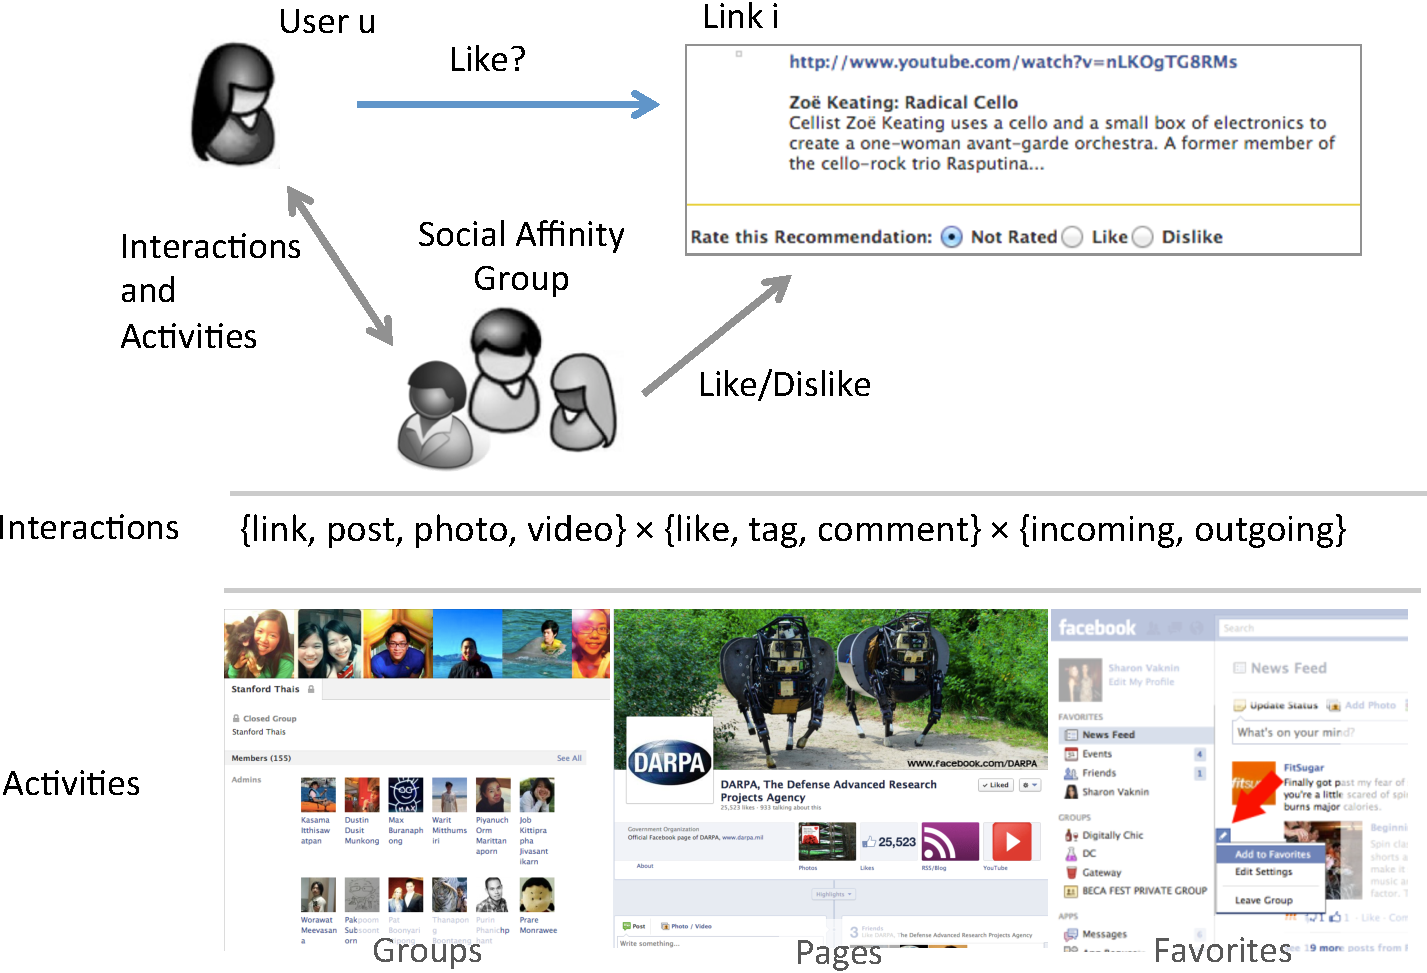
\includegraphics[width=.95\linewidth]{data/overview}
\caption{Overview of social affinity for link recommendation.}
\label{fig:overview}
\end{figure}


As illustrated in Fig~\ref{fig:overview}, the high-level objective of this paper is to predict whether or not a user $u$ will like a digital item $i$ (in our test case, a link). 
We define user $u$'s preference for link $i$ as $like(u,i)$, this will be our prediction target. 
\begin{quote}
\begin{math}
likes(u,i) =  \begin{Bmatrix}
	  True & \text{if user $u$ likes item $i$}\\
	  False & \text{otherwise}
	  \end{Bmatrix}
\end{math}
\end{quote}

We define the social affinity between two users via their direct {\em interactions}
on various digital items, and their shared {\em activities} in different communities of the social network. 
We call our recommendation algorithm \textit{Social Affinity Filtering (SAF)}, as it infers 
$like(u,i)$ through the preference of their 
\textit{ Social Affinity Groups (SAG)}, i.e. a set of users with known preferences to link $i$, and who has at least one interaction or activity in common with $u$. 

\subsection{Action types on Facebook}
On Facebook, We use the term {\em Interactions} and {\em Activities} to refer to the range of user-user and user-community actions, respectively.

\noindent {\bf Interactions} describes the communication between Facebook users. There are a few dozen different interaction types that have distinct item modality, action and direction.
\begin{itemize}
\item \textbf{Modality:} (4 possibilities)
User $u$ can interact with another user $v$ via \textit{links, posts, photos} and \textit{videos} that appear in either user's timeline.

\item \textbf{Action type:} (3 possibilities)
A user $u$ can \textit{comment} or \textit{like} 
user $v$'s item. He/she can also \textit{tag} user $v$ on an 
item, often indicating that user $v$ is present when the content is created (for photo/video/post), 
or to explicitly raise user $v$'s attention for a post -- with one exception in Facebook that $u$ cannot tag a link with users $v$ since the link is created by third parties and merely shared on Facebook.

\item \textbf{Directionality:} (2 possibilities)
We look at \textit{incoming} and \textit{outgoing} interactions, i.e.,
if user $u$ comments on, tags, or likes user $v$'s item,
then this is an outgoing interactions for $u$, and an incoming interactions for $v$.
Although high correlation between \textit{incoming} and \textit{outgoing} interactions 
is recently observed~\cite{saez2011high}, whether or not interaction direction 
affects user preferences differently is still an open question we wish to answer
in this work. 
%then $u$ is in the set of incoming interactions for $v$
%and $v$ is in the set of outgoing interactions for $u$.
      								
\end{itemize}
There are a total of 22 interaction types. Namely the cross-product of modalities, actions and directions, minus {\em link-tag-\{incoming, outgoing\}}. 

%\subsection{Activities}
\noindent{\bf Activities} describes the user interactions with Facebook communities like groups, pages, favourites.
\begin{itemize}
  %@SCOTT/LEXING following defination are taken from facebook blog. I am confused how to cite it %
  \item \textbf{Groups} on Facebook 
\footnote{According to Facebook Blog (\surl{https://www.facebook.com/blog}), ``Groups are the place for small group communication and for people to share their common interests and express their opinion. Groups allow people to come together around a common cause, issue or activity to organize, express objectives, discuss issues, post photos and share related content''. 
\label{fn:fbblog}}
are analogous to community organizations in the real-world. It allows users to declare membership and supports people to organize activities, to post related content, and to have recurring discussions about them.  Examples of groups include {\em Stanford Thai} (Fig~\ref{fig:overview} bottom left), or {\em Harvard Debate Club}.
  \item \textbf{Pages} on Facebook
  \footnote{According to Facebook Blog, ``Facebook Pages enable public figures, businesses, organizations and other entities to create an authentic and public presence on Facebook. Facebook Pages are visible to everyone on the internet by default. Facebook user can connect with these Pages by becoming a fan and then receive their updates and interact with them.'' }
  %\footnotemark[\ref{fn:fbblog}] 
  are analogous to the homepages of people, organizations and events on the world-wide-web. They are publicly visible, and users can subscribe to the updates on the page, and also engage in discussions. Example pages include {\em DARPA} (an organization, Fig~\ref{fig:overview} bottom middle), or {\em Beyonce} (a singer).

  \item \textbf{Favourites} are analogous to bookmarks (on physical books or on the web browser). It it is a user-created list containing various digital items such as Facebook apps, books, music, and many other types of items to indicate their interest. Example favourite items include {\em Big Bang Theory} (TV series), or {\em FC Barcelona} (soccer club). Fig~\ref{fig:overview} bottom right show a Facebook screenshot when a user adds a favourite.
  \footnote{According to Facebook Blog, ``Facebook facilitates a wide variety of user selected favourites (Activities, Favorite Athletes, Books, Interests, Movies, Music, Sports, Favorite Teams, Television). These favourites allow a user to associate themselves with other people who share their same favourite tendencies.}
\end{itemize} 

Our evaluation includes thousands of active {\em group}, {\em page} or {\em favourite} features, details of them can be found in Sec~\ref{sec:datadesc}.

Note that the notion of affinity we adopt is based on direct user {\em actions}, rather than
static profile information, or structural information of the social graph. 
We believe this is a useful view into the social network, as it was recently pointed out
that a user's attention (i.e., interactions) are divided among a small subset of Facebook friends~\cite{backstrom2011center}, and that ratings of real-world friendship strength seems to be more predictable from the intimacy, intensity, and duration of interactions, than from social distance and structural information~\cite{gilbert2009predicting}. Our affinity definition is based on direct interactions within a users' ego network, this is complementary to 
a recent alternative~\cite{Panigrahy2012ubr} that uses number of paths between two users encodes the resilience of network structure, 
as it was recently found~\cite{Goel2012structure} that the vast majority of information diffusion
happens within one step from the source node. 
% interactions
%Our affinity
%\cite{Wilson2012BSG}


\subsection{Social Affinity Groups}
\label{ssec:sag}

\eat{
The major objective of this paper is to evaluate the effectiveness of \textit{Social Affinity Filtering (SAF)} and fine grained 
analysis of the informativeness of Interactions and Activities.We divide our recommendation algorithm into two categories based 
on Interactions and Activities of 
}

Based on the definitions of {\em interaction}  and {\em activities} above, 
%\textit{ Social Affinity Groups (SAG)} with target item, 
we define two types of {\em social affinity groups} of a user with a target item,
namely \textit{Interaction  Social Affinity Groups (ISAG)} and \textit{Activity Social Affinity Groups (ASAG)}.

\begin{itemize}
  \item \textbf{Interaction  Social Affinity Groups}. Let the set of interaction affinity classes be the cross-product of 
  Interaction modality, action and direction:
  \begin{quote}
  \begin{math}
  	\textit{Interaction Affinity Classes} = \{link, post, photo, video\} \times \{like, tag, comment\} \times \{incoming, outgoing\}
  \end{math}
  \end{quote}
  %Additionally, we add friendship interaction affinity class. \\
  We define 
  \begin{quote}
  \textit{ISAG(u, k)} $:=$ the set of the users who have interaction $k$ with user $u$.
  \end{quote}
   For example,
   \begin{quote}
   
   \textit{ISAG(u, link-like-incoming)}  is the set of all users who have liked link posted by user $u$. \\
   \textit{ISAG(u, photo-comment-outgoing)} is the set of all users whose photos received at least one comment from $u$. \\
   \end{quote}
\item \textbf{Activity Social Affinity Groups}: We define activity affinity groups based on group membership, page likes and user favourites.
	\begin{quote}
	\textit{ASAG(u, k)} $:=$ the set of the users who have common preference for entity $k$ (group, page, favourite) with user $u$.   
	\end{quote}
\end{itemize}


\subsection{Social Affinity Features}
\label{ssec:SAfeature}

\begin{itemize}
  \item \textbf{Interaction Social Affinity Features} : We define Interaction affinity features for target user $u$ and item $i$ for ISAG's classes 
  $ \langle X_{1},X_{2}\ldots,X_{k}\rangle$ as
  \begin{quote}
  \begin{math}
   X_{k,u,i} = \begin{Bmatrix}
   		True & if\ \exists v\in ISAG(u,k) \wedge likes(v,i)\\ \\
   		False & otherwise
   \end{Bmatrix}
  \end{math}
  \end{quote}
  Additionally we add friend feature which encodes whether the target item $i$ is liked by friend or not.
  \item \textbf{Activity Social Affinity Features} : We define activity affinity features for target user $u$ and item $i$   \
  $ \langle X_{1},X_{2}\ldots,X_{k}\rangle$ as\\ \\
  \begin{math}
   X_{k,u,i} = \begin{Bmatrix}
   		True & if\ \exists\ v\in \ ASAG(u,k) \wedge likes(v,i)\\ \\
   		False & otherwise
   \end{Bmatrix}
  \end{math}
	In our analysis we use only those features(groups, pages and favourites) that are joined/liked by at least one of our app users.
\end{itemize}

\eat{
%% SCOTT already covered these elsewhere
We train naive bayes, Logistic Regression(LR) and Support Vector Machine(SVM) model with affinity features.
Logistic Regression and SVM algorithm was implemented using \textit{LIBLINER} \cite{liblinear} package. 
We define Constant predictor as baseline predictor. Constant predictor predicts the most common outcome in our datase ie disliket.
We compare the performance of Social Affinity Filtering with the state of the art social collaborative filtering technique 
Social MatchBox(SMB)\cite{SMB}.

In real world social networks activity features grows very quickly as number of user in social network increases. This motivates the fine grained
analysis of informativeness of social affinity features. Furthermore, fine grained analysis of interactions helps to understand the nature of user-user 
interactions and its predictiveness in greater detail. Hence, for the analysis of activities and interactions we rank the features using
\textit{Conditional Entropy}. 
\textit{Conditional Entropy} is defined as
\begin{quote}
\begin{math}
H(Y|X=True) = \\-\sum_{y\in{(like,dislike)}} p(y|X$=$true)$ $log( p(y|X$=$true))
\end{math}
\end{quote}

With the data and methodology now defined including all dimensions of our analysis, we now proceed to an in-depth discussion of our findings.
}




 






\section{Evaluation}

\begin{itemize}
  \item Page likes are most predictive followed by group and favourites
   \item For Large social networks encoding user's membership(group/pages/favourites) as features and performing matrix factorization is not scalable (as there are millions of groups/pages/activities). This research shows that the memebership can be directly plugged into existing highly scalable algorithms to achieve better accuracy than state of art matrix factorization techniques. 
\end{itemize}


\begin{figure*}
\centering
\begin{tabular}{cc}
\subfloat[Fig: Friend and NonFriend Recommended Data][Friend and NonFriend Recommended Links]{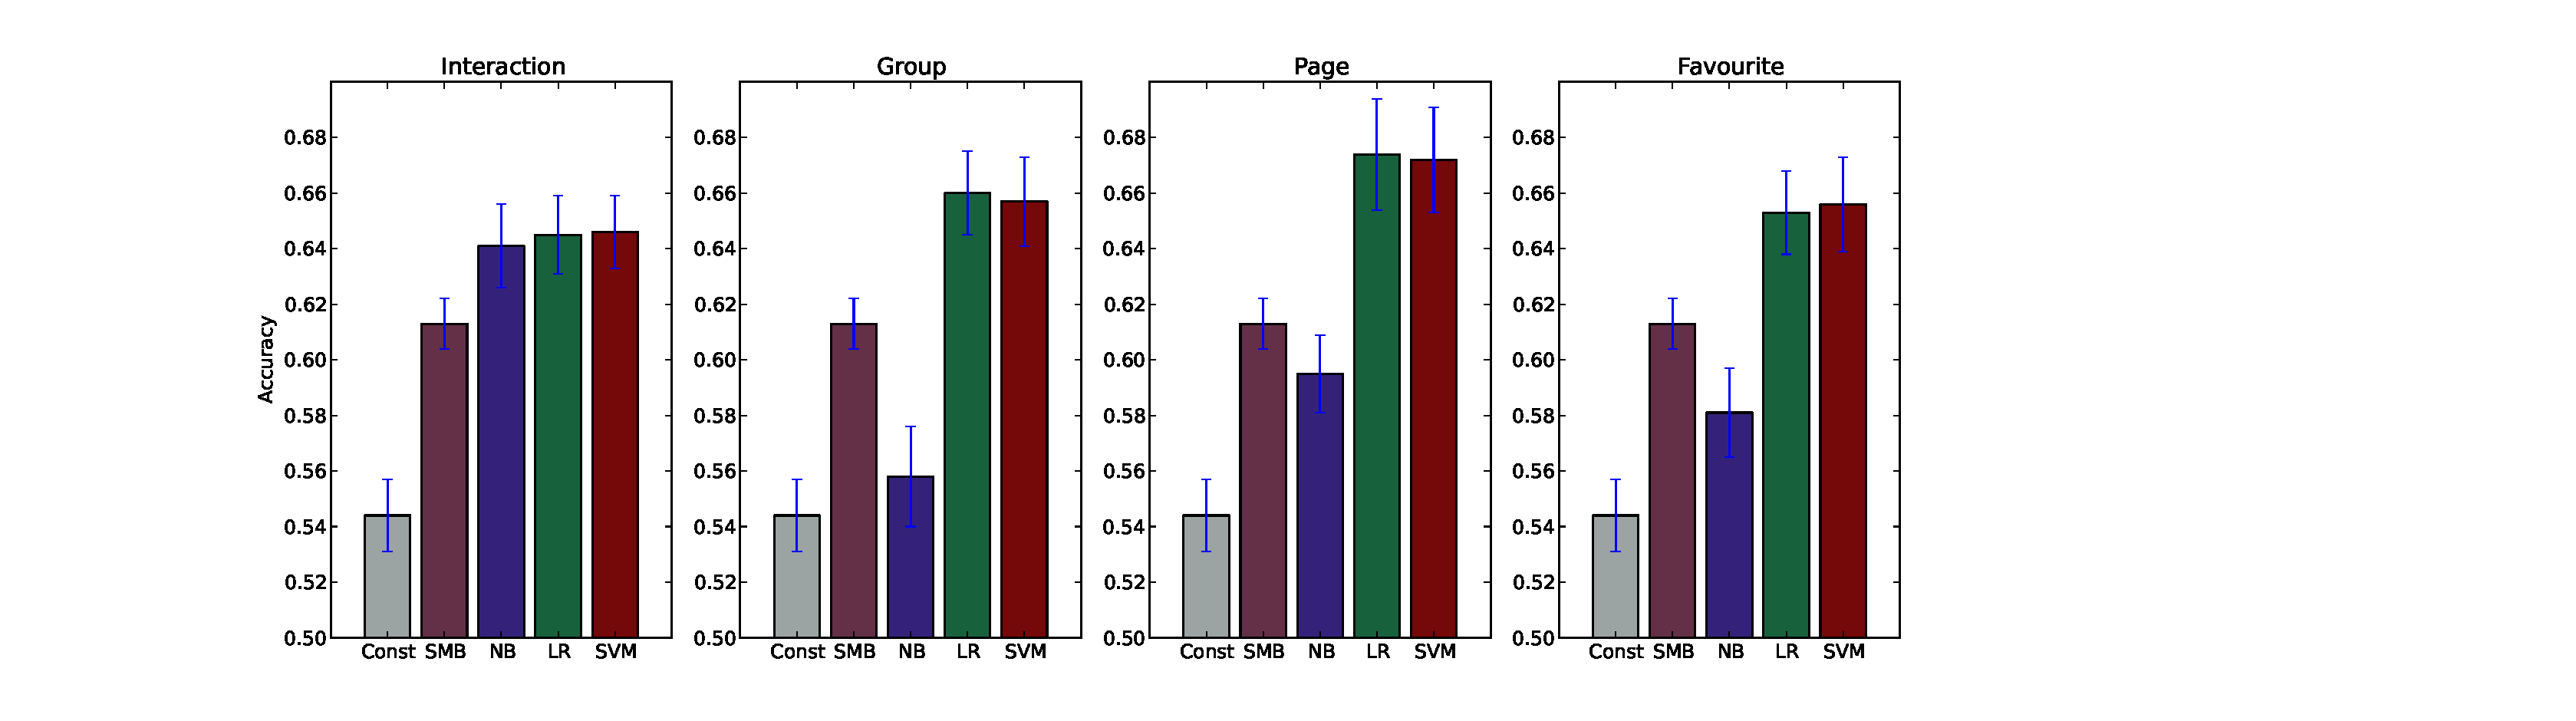
\includegraphics[scale=0.25]{data/plots/accuracy/accuracy.eps}}
\subfloat[Fig: Friend Recommended Data][Friend Recommended Links]{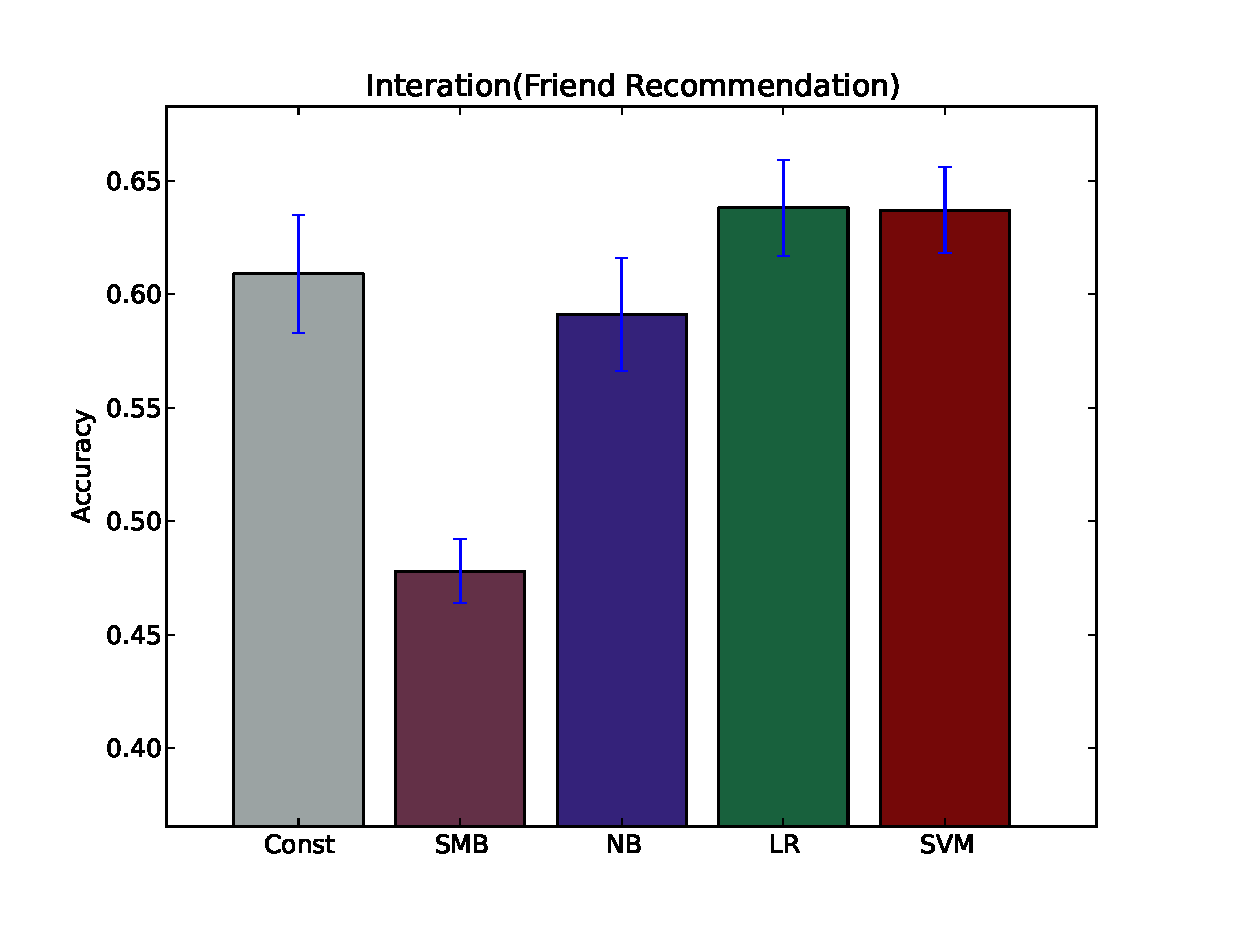
\includegraphics[height=38mm, width=28mm]{data/plots/accuracy/friendRecommendation.eps}}
\end{tabular}
\caption{Accuracy of predictors (constant, social matchbox, naive bayes, logistic regression, SVM) for interation, group, page, favourite features}
\label{Fig: Accuracy}
\end{figure*}

%\begin{figure*}
%\centering
%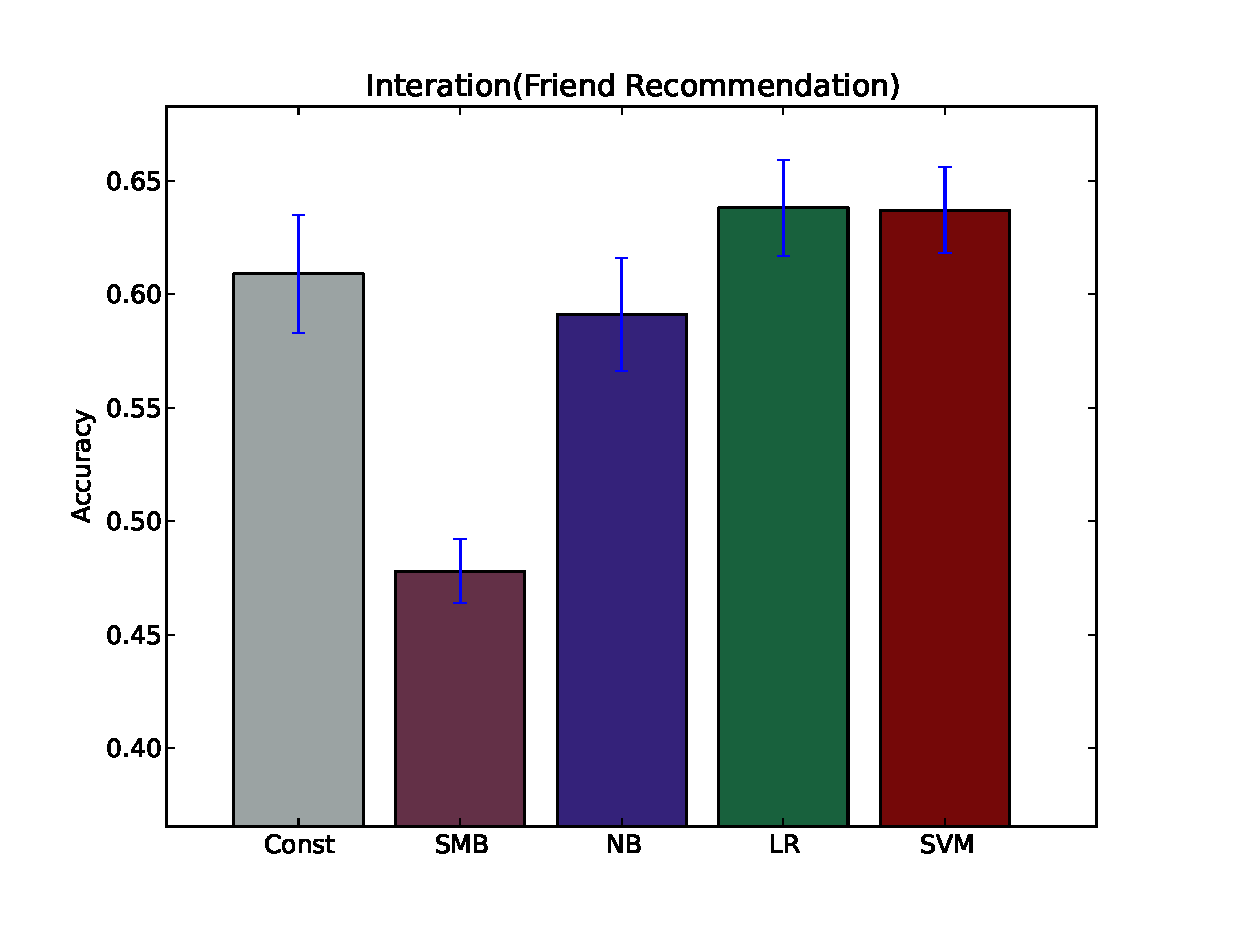
\includegraphics[height=45mm, width=30mm]{data/plots/accuracy/friendRecommendation.eps}
%\caption{Accuracy of predictors (constant, social matchbox, naive bayes, logistic regression, SVM) based on interaction features for friend recommended links}
%\label{Fig: Accuracy}
%\end{figure*}

\begin{figure*}
\centering
\begin{tabular}{c}
\subfloat[Fig: Conditional Entropy vs Group Size][conditional entropy vs group size (top 500)]{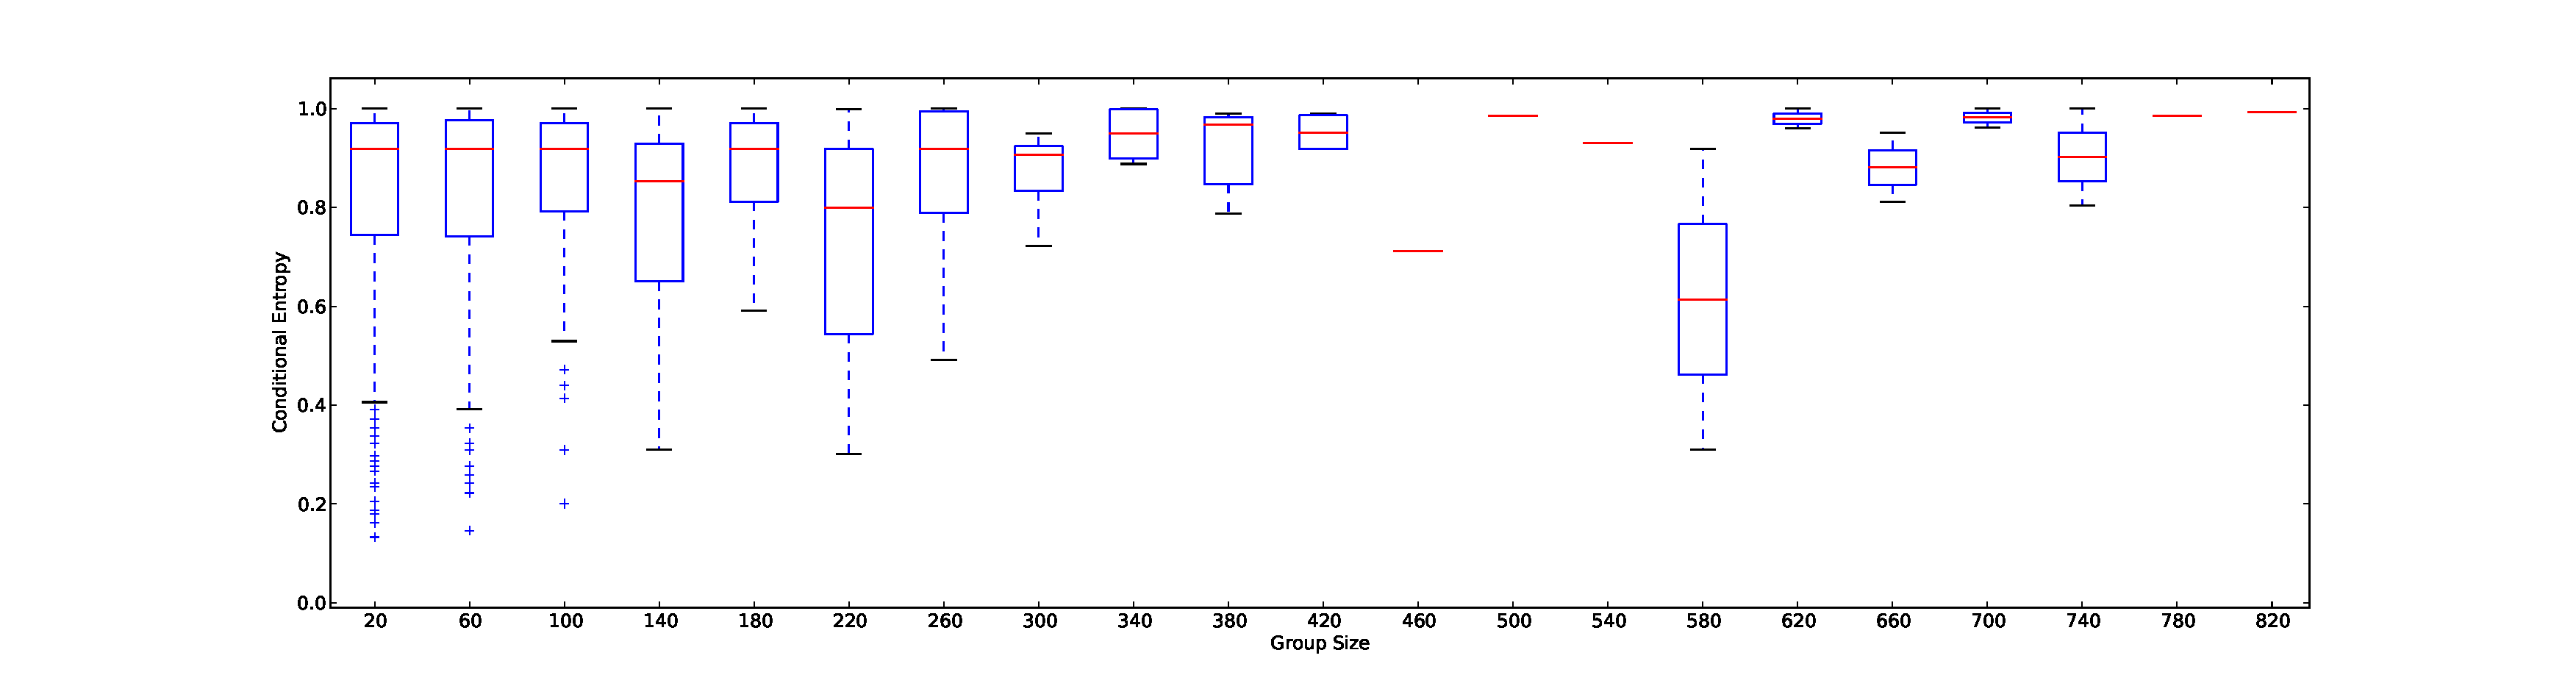
\includegraphics[height=40mm,width=150mm]{data/plots/boxPlots/CEvsGroupSize.eps}}\\
\subfloat[Fig: Conditional Entropy vs Page Size][conditional entropy vs page size (top 1000)]{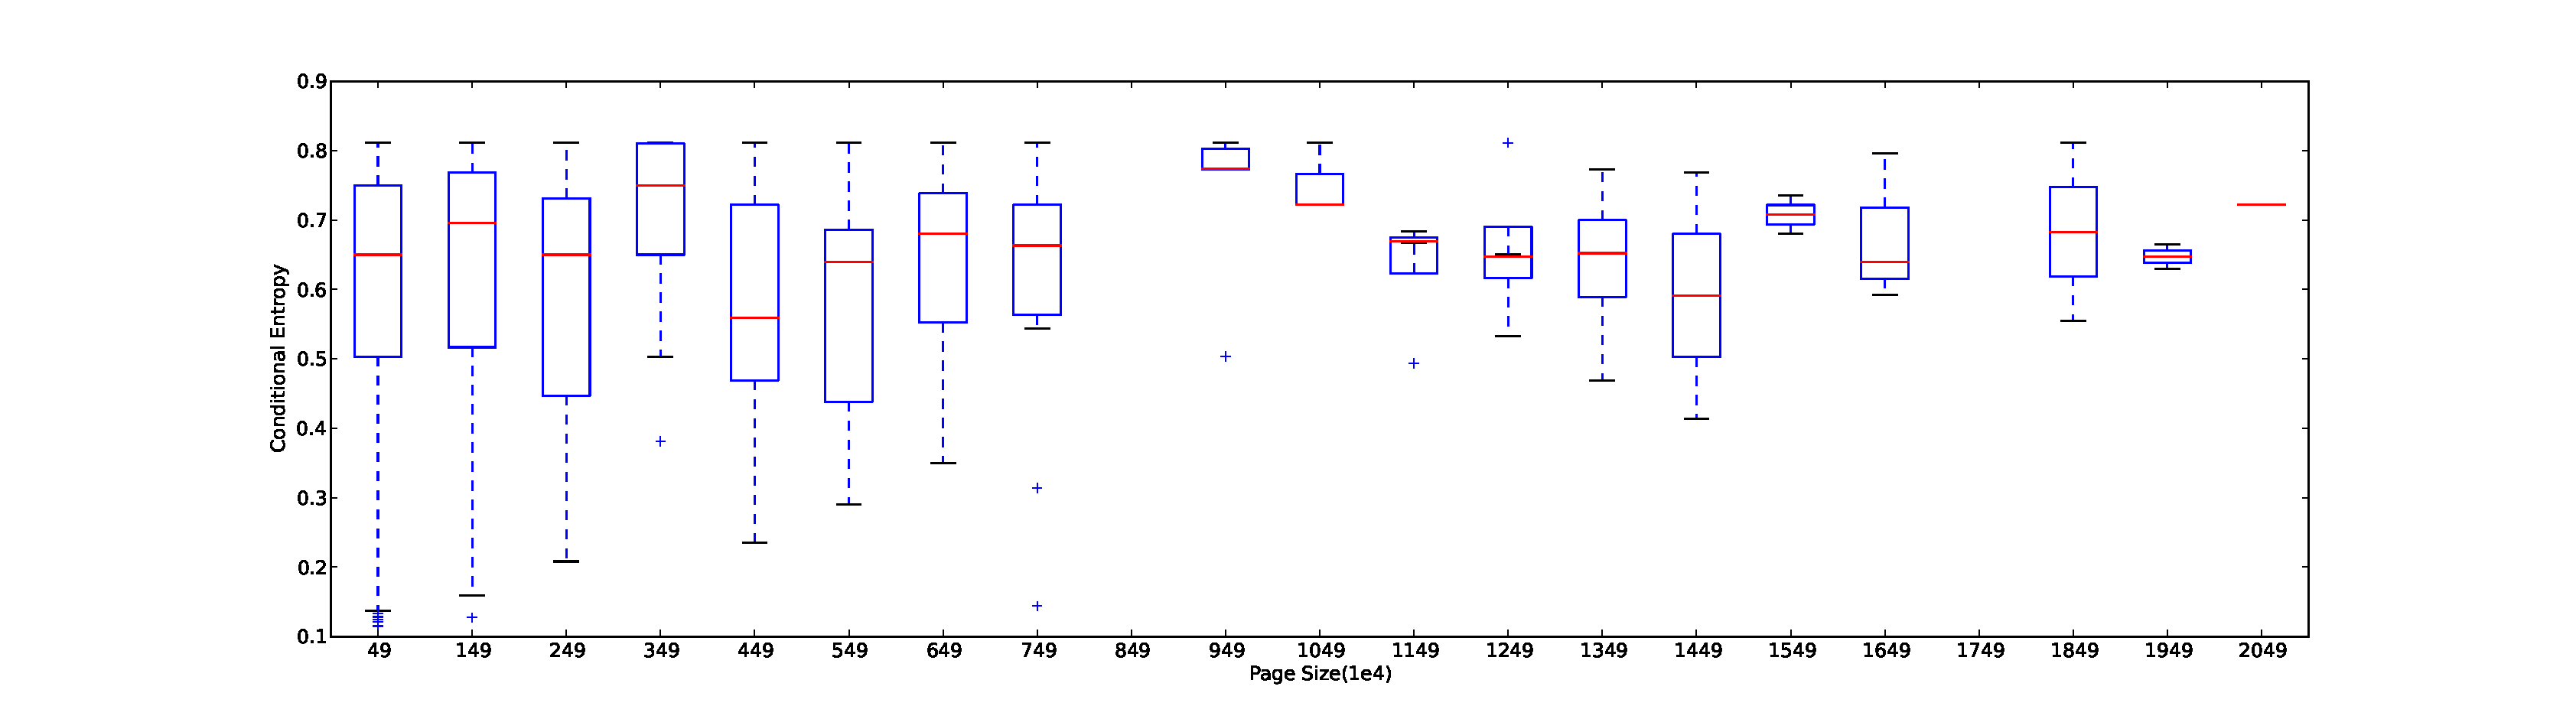
\includegraphics[height=40mm,width=150mm]{data/plots/boxPlots/CEvsPageSize.eps}}\\
\subfloat[Fig: Conditional Entropy vs Favourites Size][conditional entropy vs favourites size (top 800)]{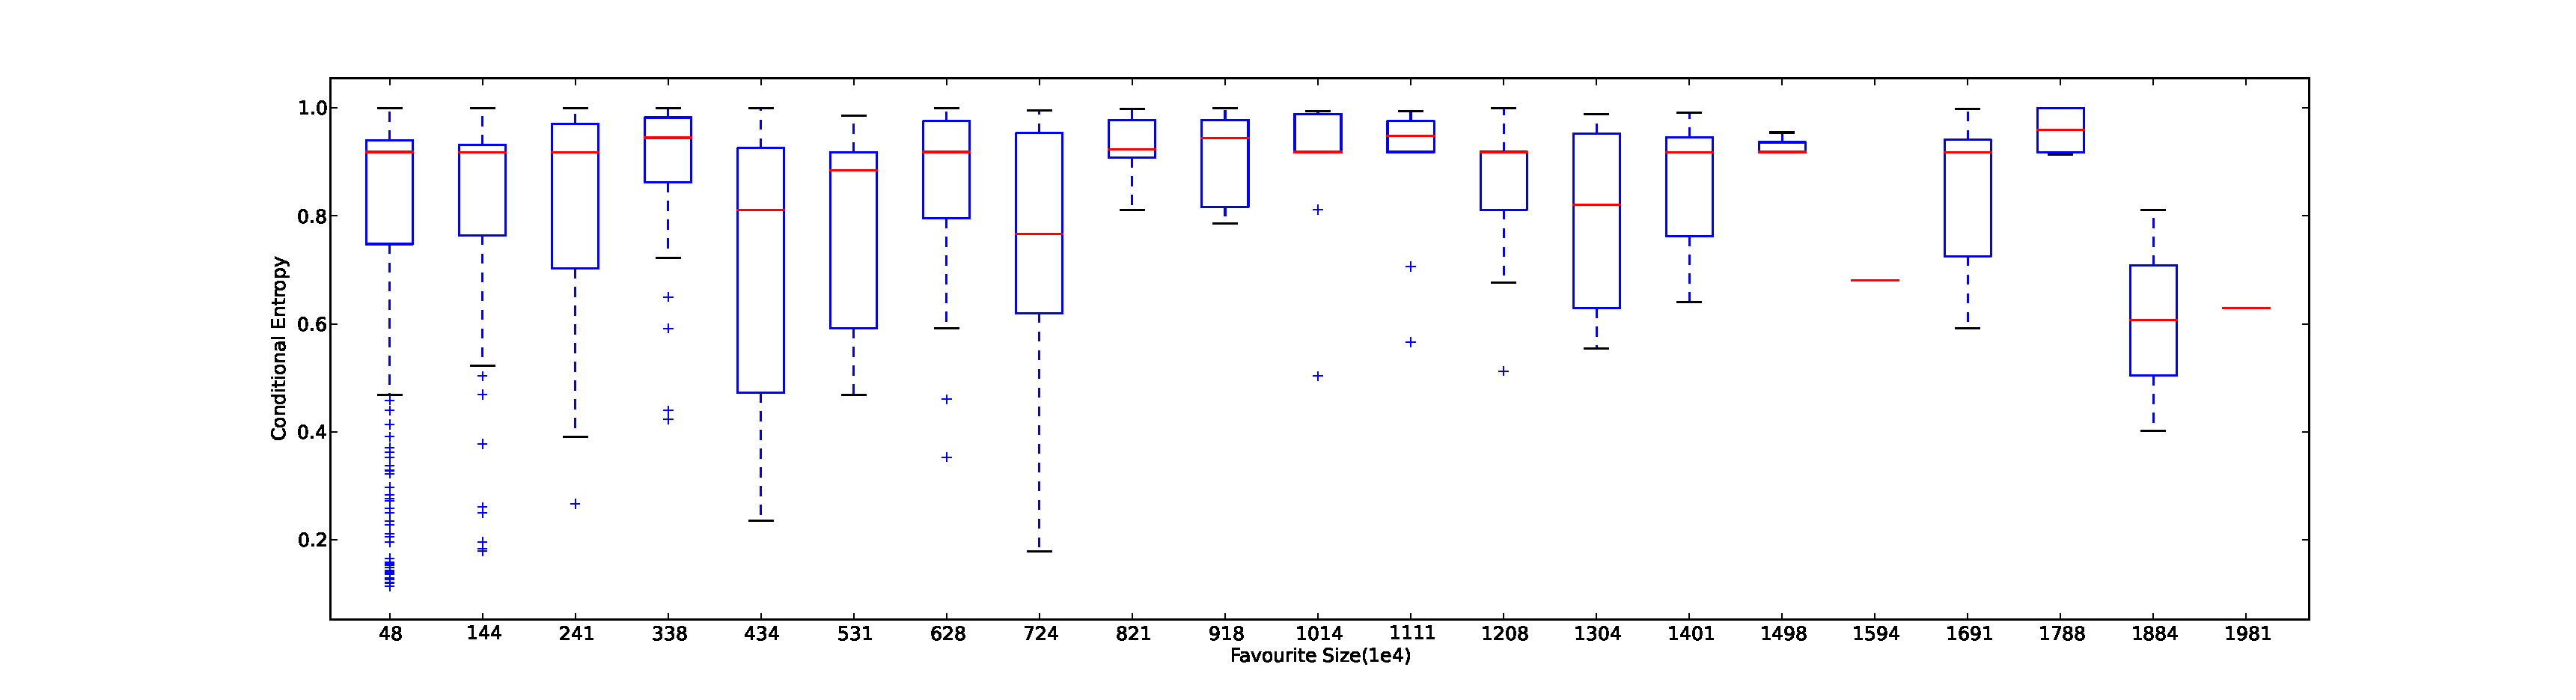
\includegraphics[height=40mm,width=150mm]{data/plots/boxPlots/CEvsFavouriteSize.eps}}
\end{tabular}
\caption{conditional entropy vs size (top k)}
\label{Fig: conditional entropy vs size(top k) Box plots}
\end{figure*}

\begin{figure*}
\centering
\begin{tabular}{c}
\subfloat[Fig: mutual information vs Group Size][mutual information vs group size (top 500)]{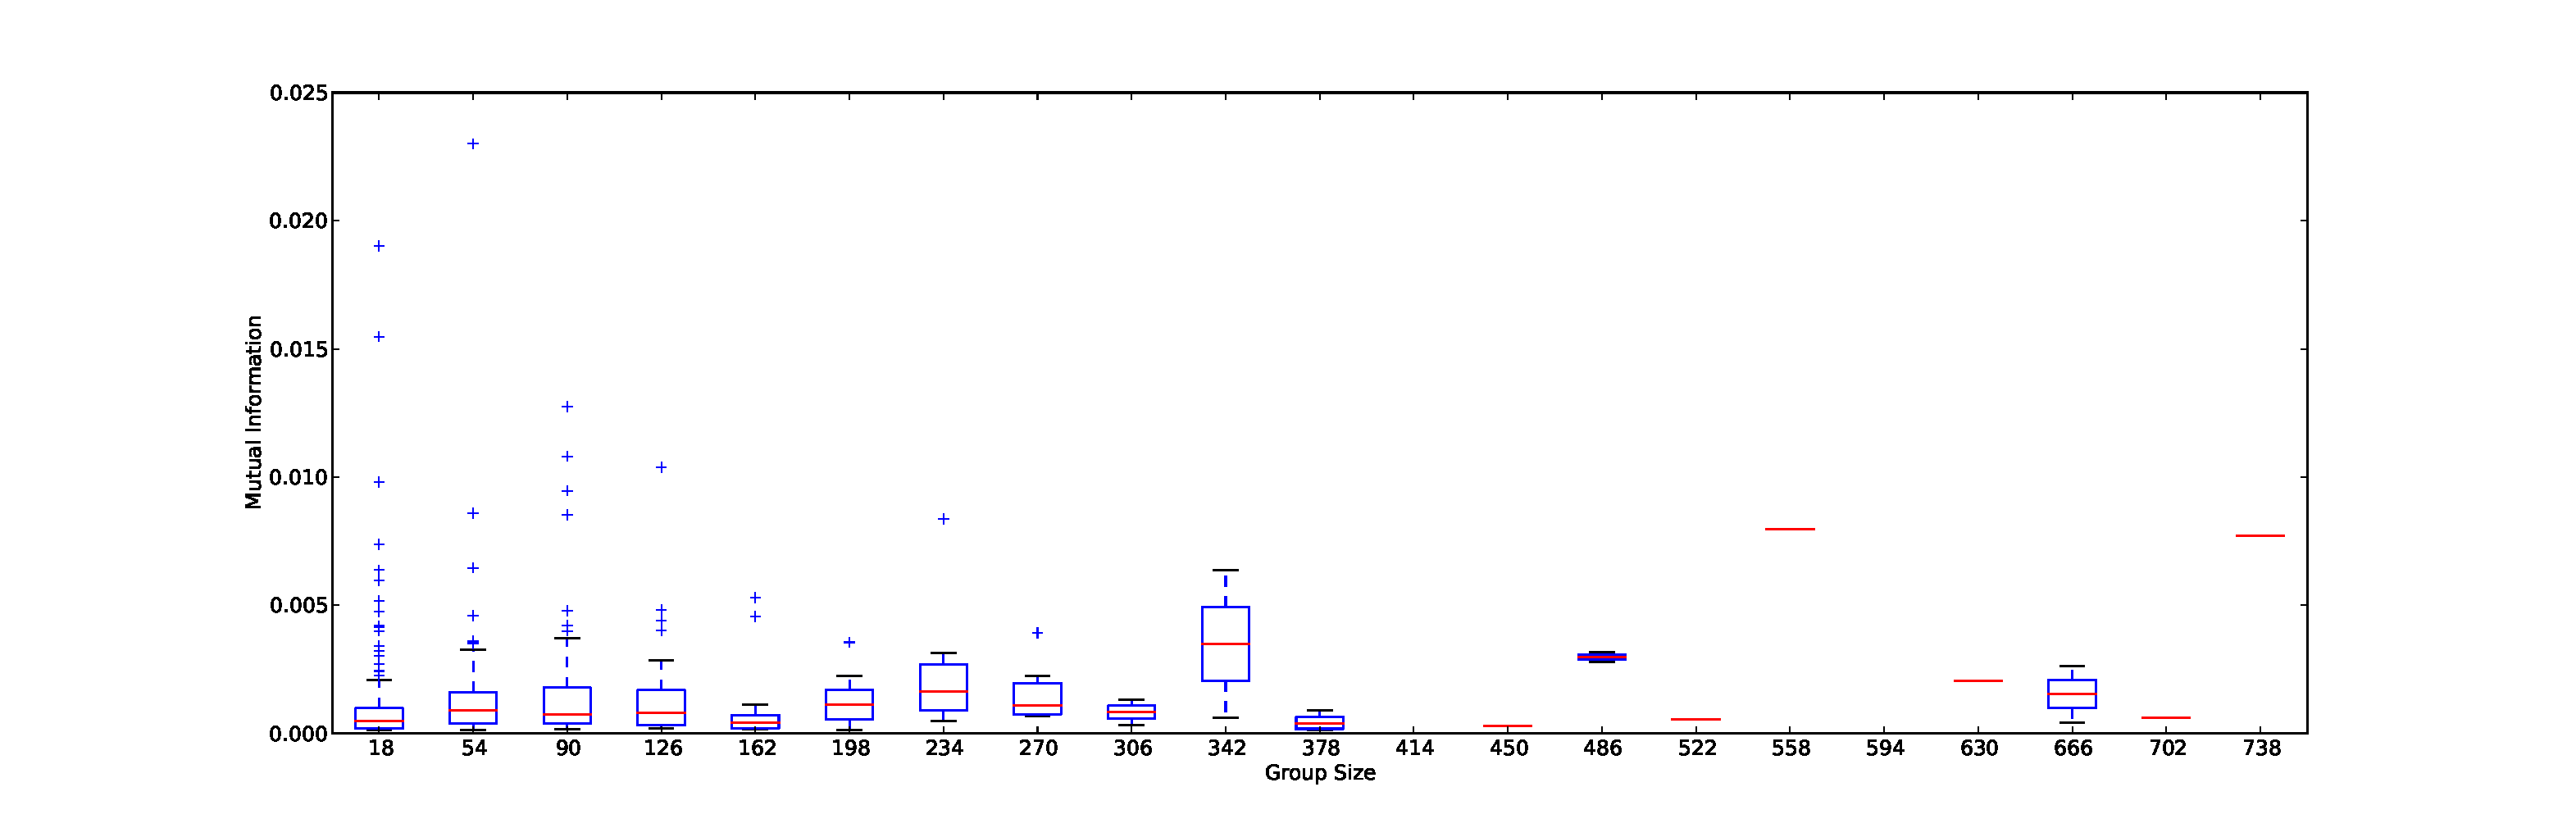
\includegraphics[height=40mm,width=150mm]{data/plots/boxPlots/MIvsGroupSizeTop500.eps}}\\
\subfloat[Fig: mutual information vs Page Size][mutual information vs page size (top 1000)]{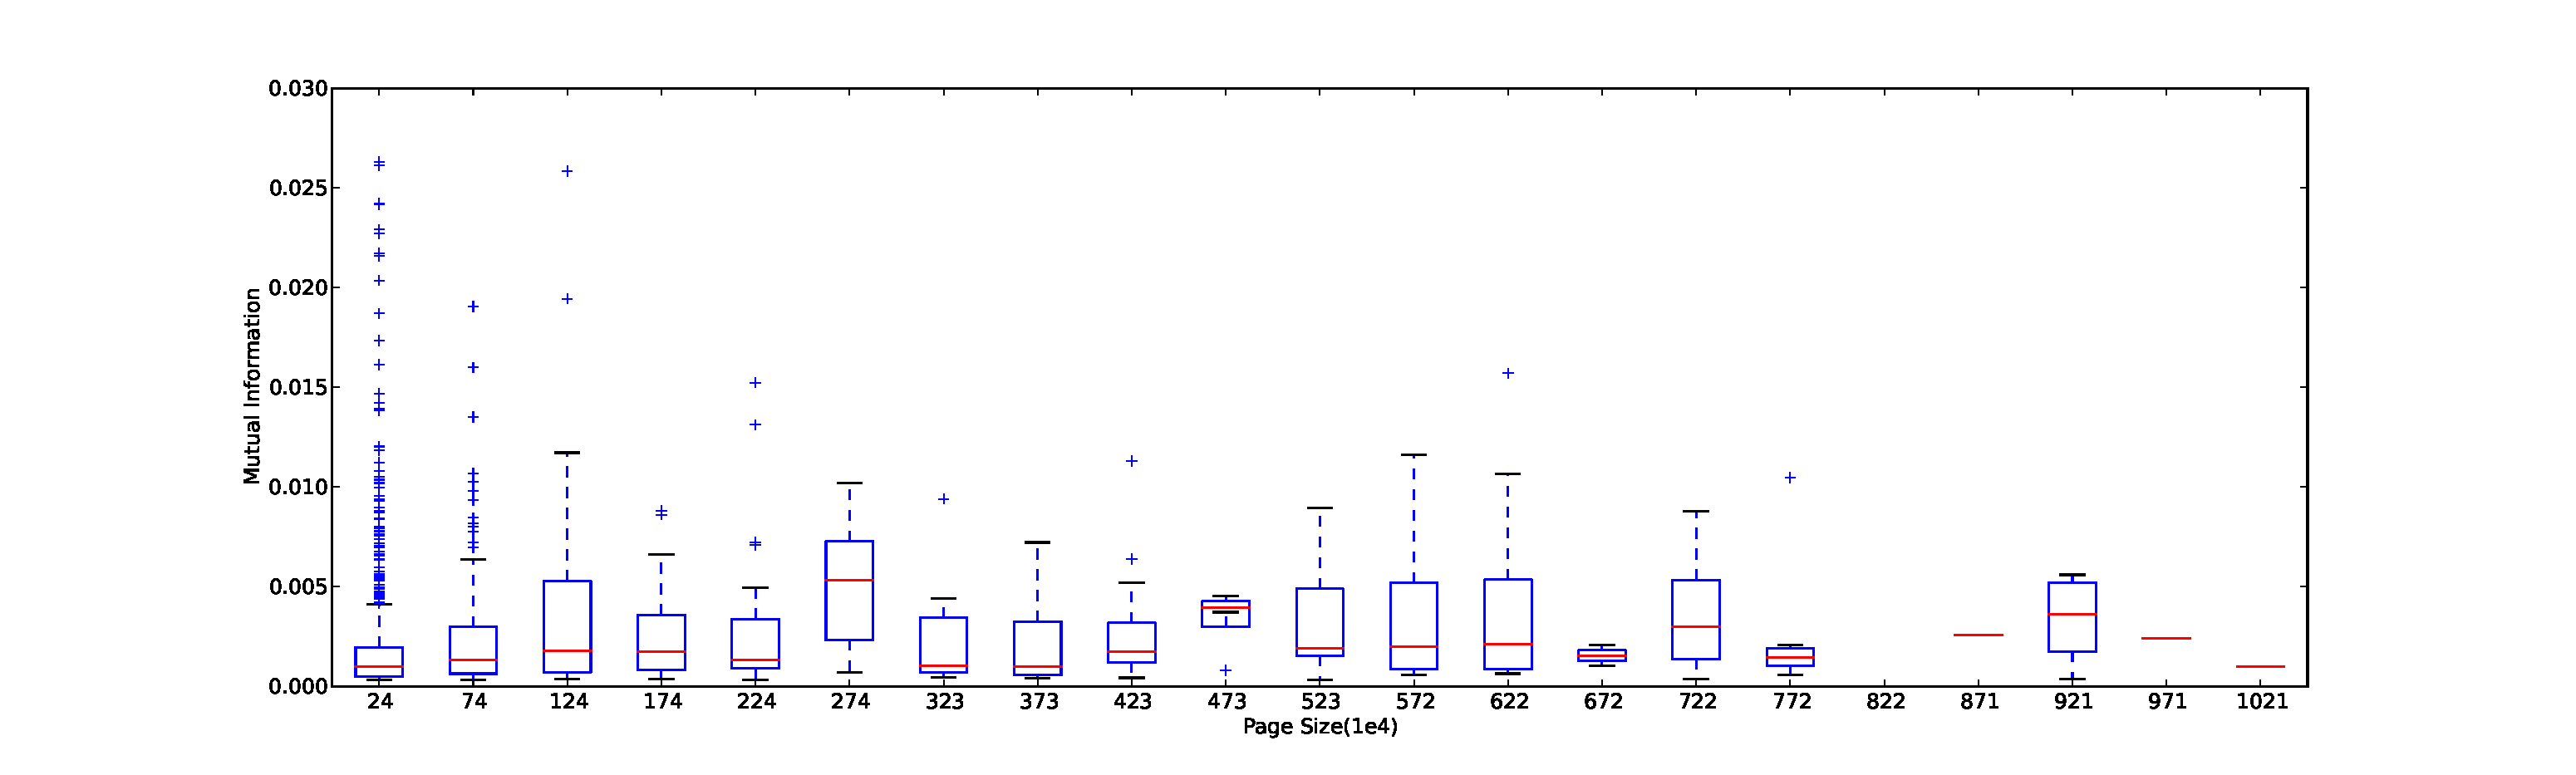
\includegraphics[height=40mm,width=150mm]{data/plots/boxPlots/MIvsPageSizeTop1000.eps}}\\
\subfloat[Fig:  mutual information vs Favourites Size][mutual information vs favourites size (top 800)]{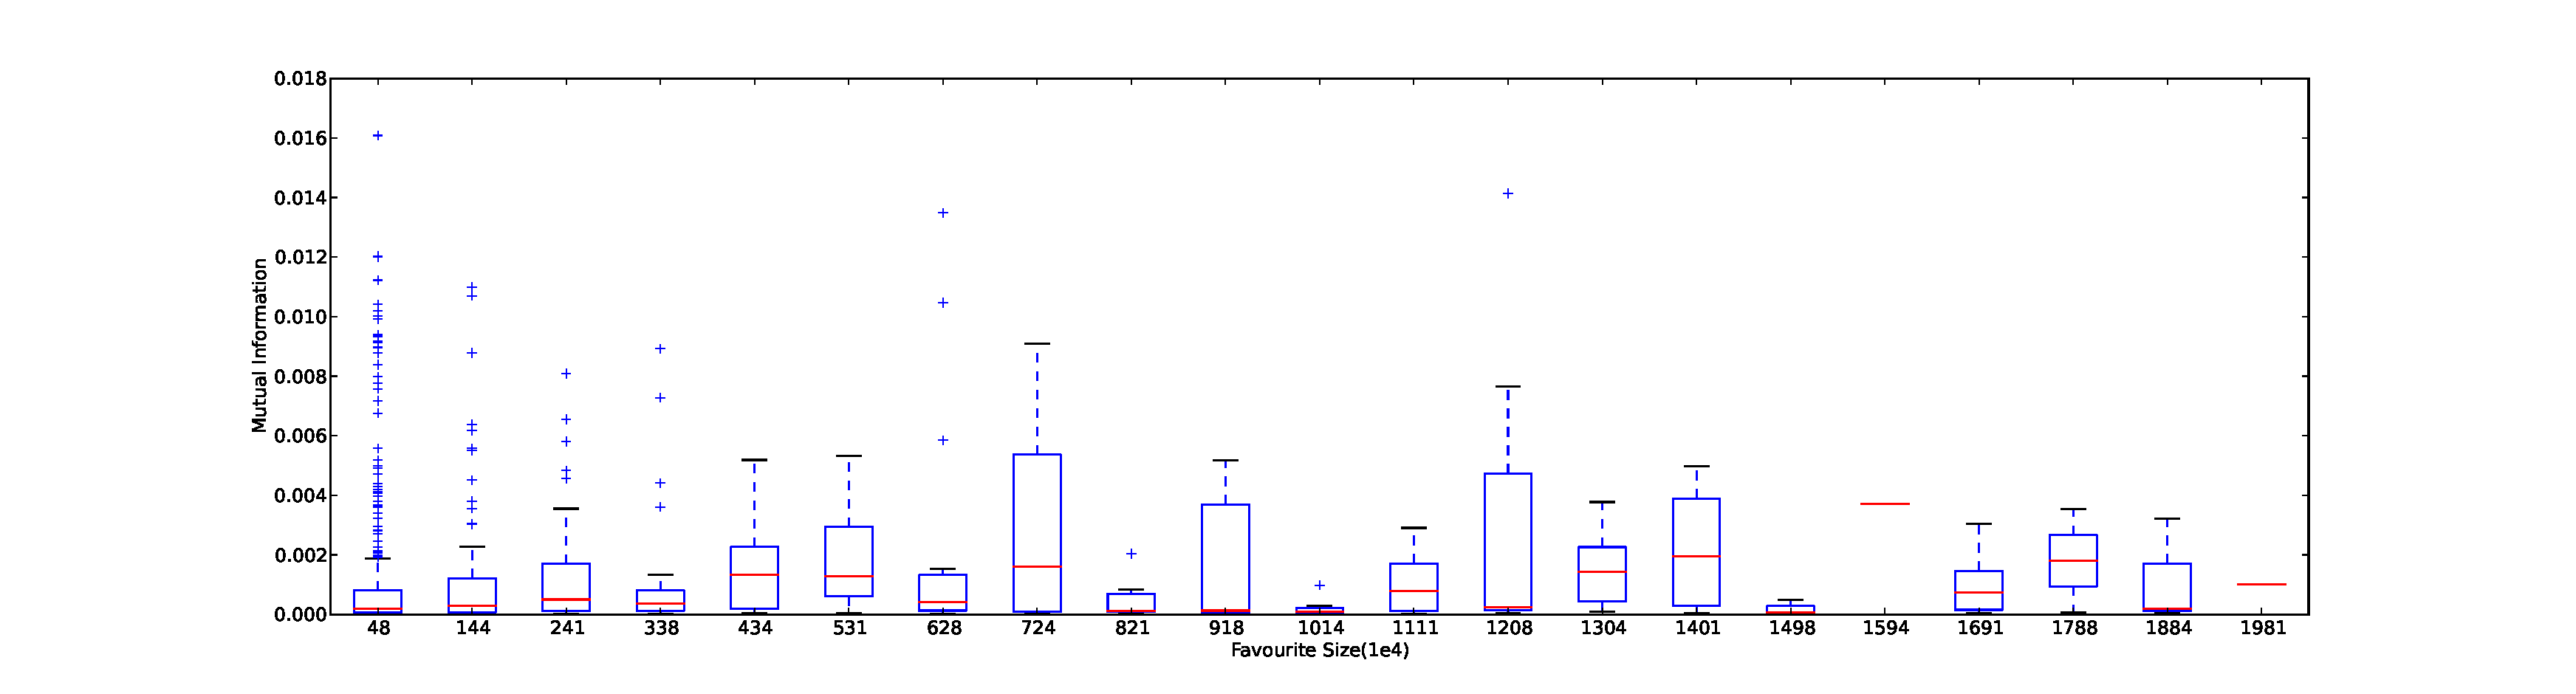
\includegraphics[height=40mm,width=150mm]{data/plots/boxPlots/MIvsFavSizeTop800.eps}}
\end{tabular}
\caption{ mutual information  vs size (top k)}
\label{Fig: mutual information  vs size(top k) Box plots}
\end{figure*}

\begin{figure*}
\centering
\begin{tabular}{c}
\subfloat[Fig: mutual information vs Page Size][mutual information vs page size (top 1000)]{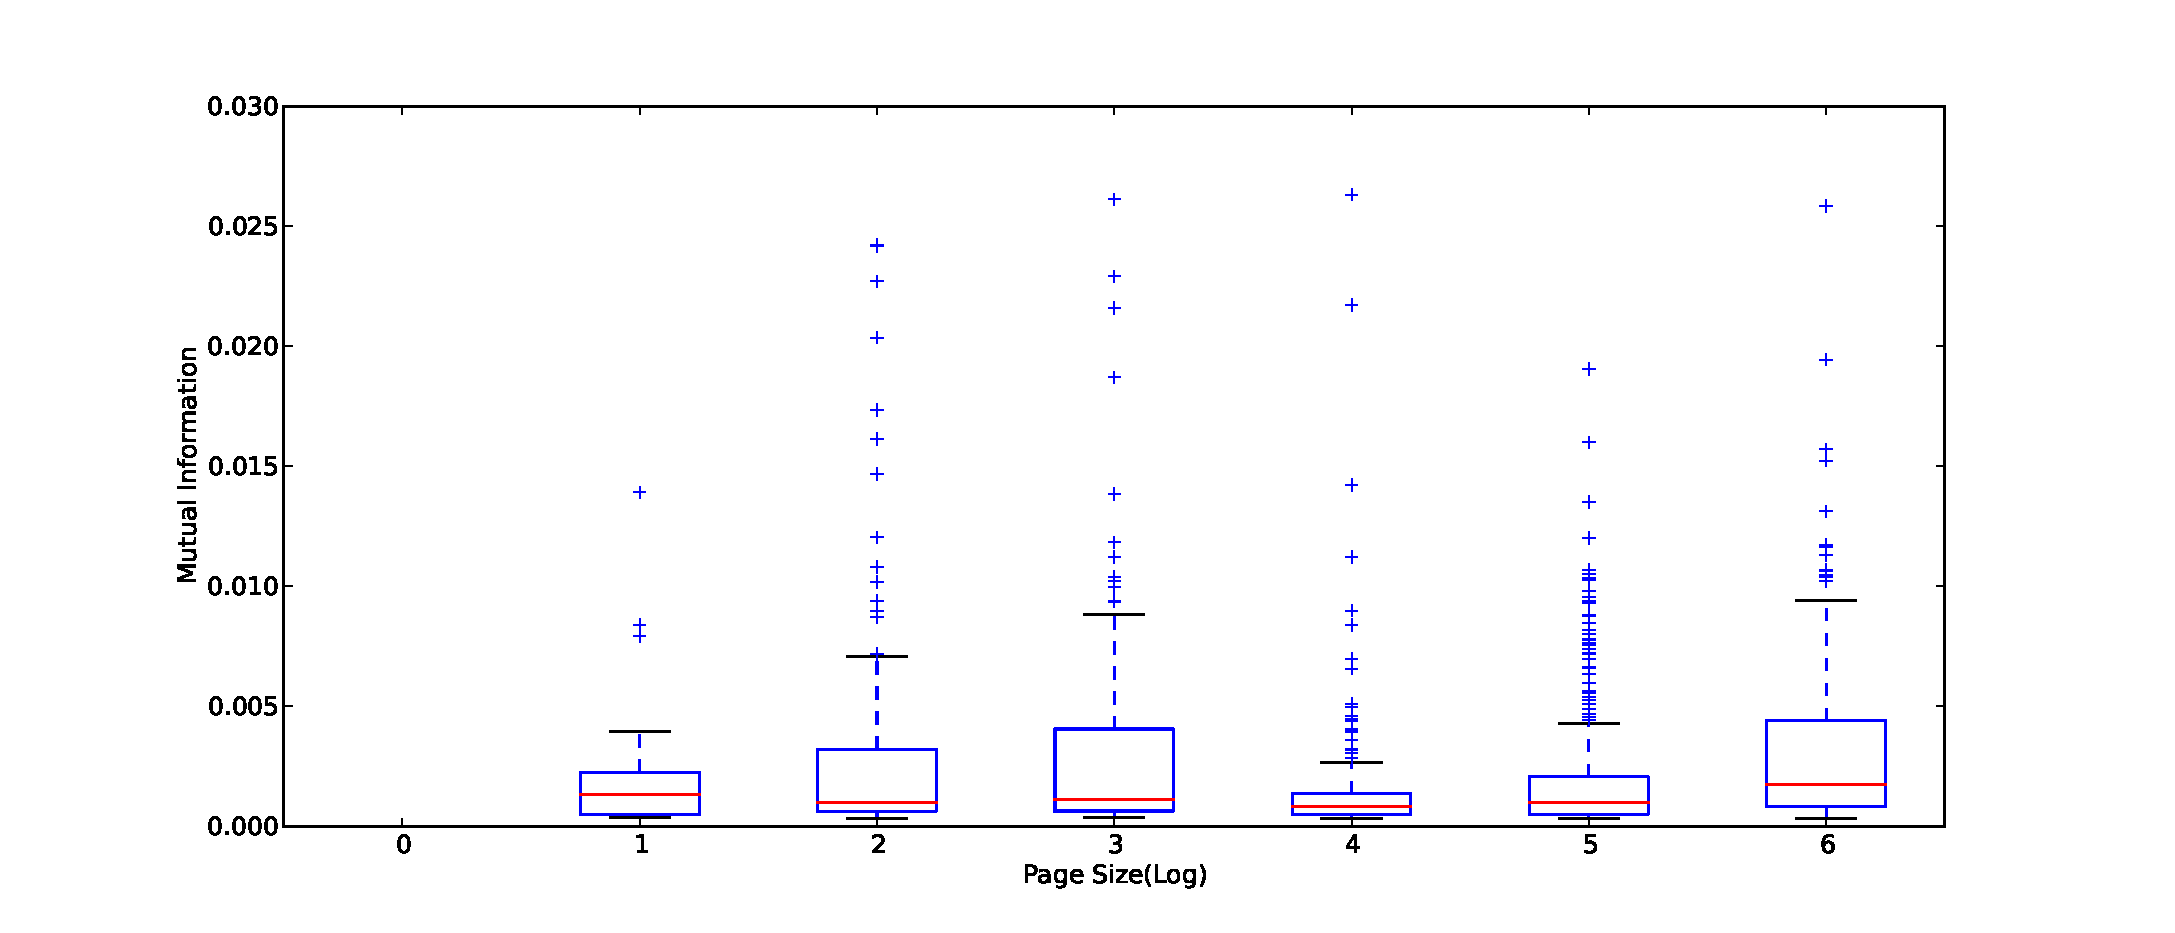
\includegraphics[height=40mm,width=150mm]{data/plots/boxPlots/MIvsPageSizeLogtop1000.eps}}\\
\subfloat[Fig:  mutual information vs Favourites Size][mutual information vs favourites size (top 800)]{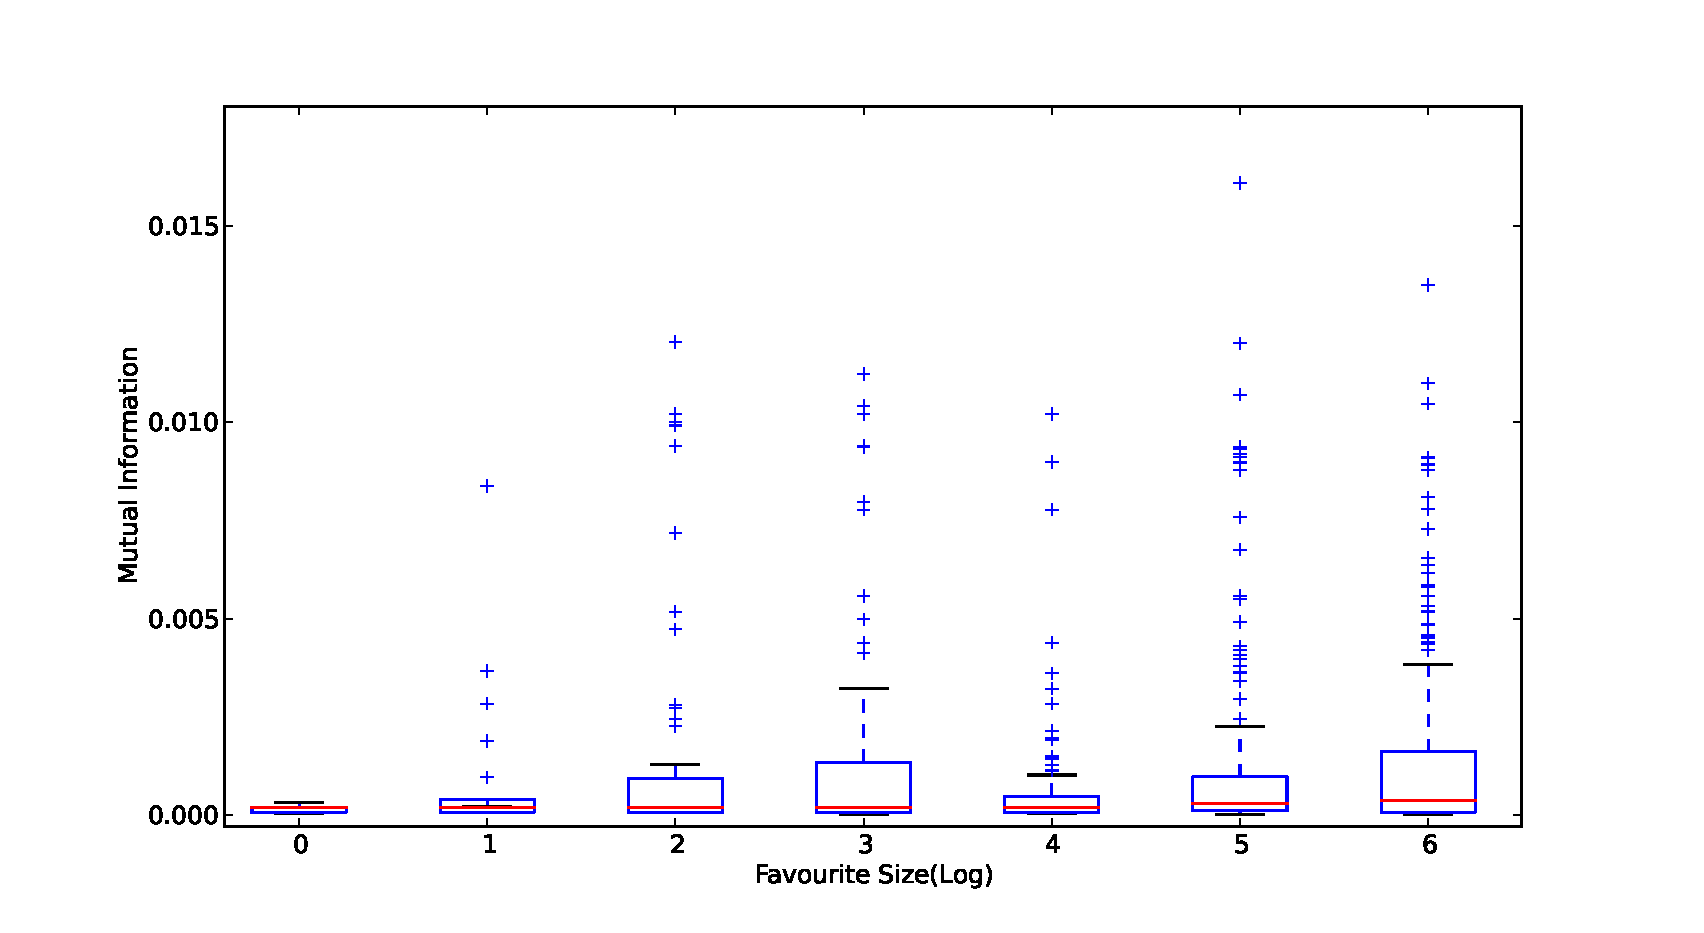
\includegraphics[height=40mm,width=150mm]{data/plots/boxPlots/MIvsFavSizeLogtop800.eps}}
\end{tabular}
\caption{ mutual information  vs size (top k)}
\label{Fig: mutual information  vs size(top k) Box plots}
\end{figure*}

\begin{figure*}
\centering
\begin{tabular}{c}
\subfloat[Fig:  conditional entropy vs favourite categories][ conditional entropy vs favourite categories]{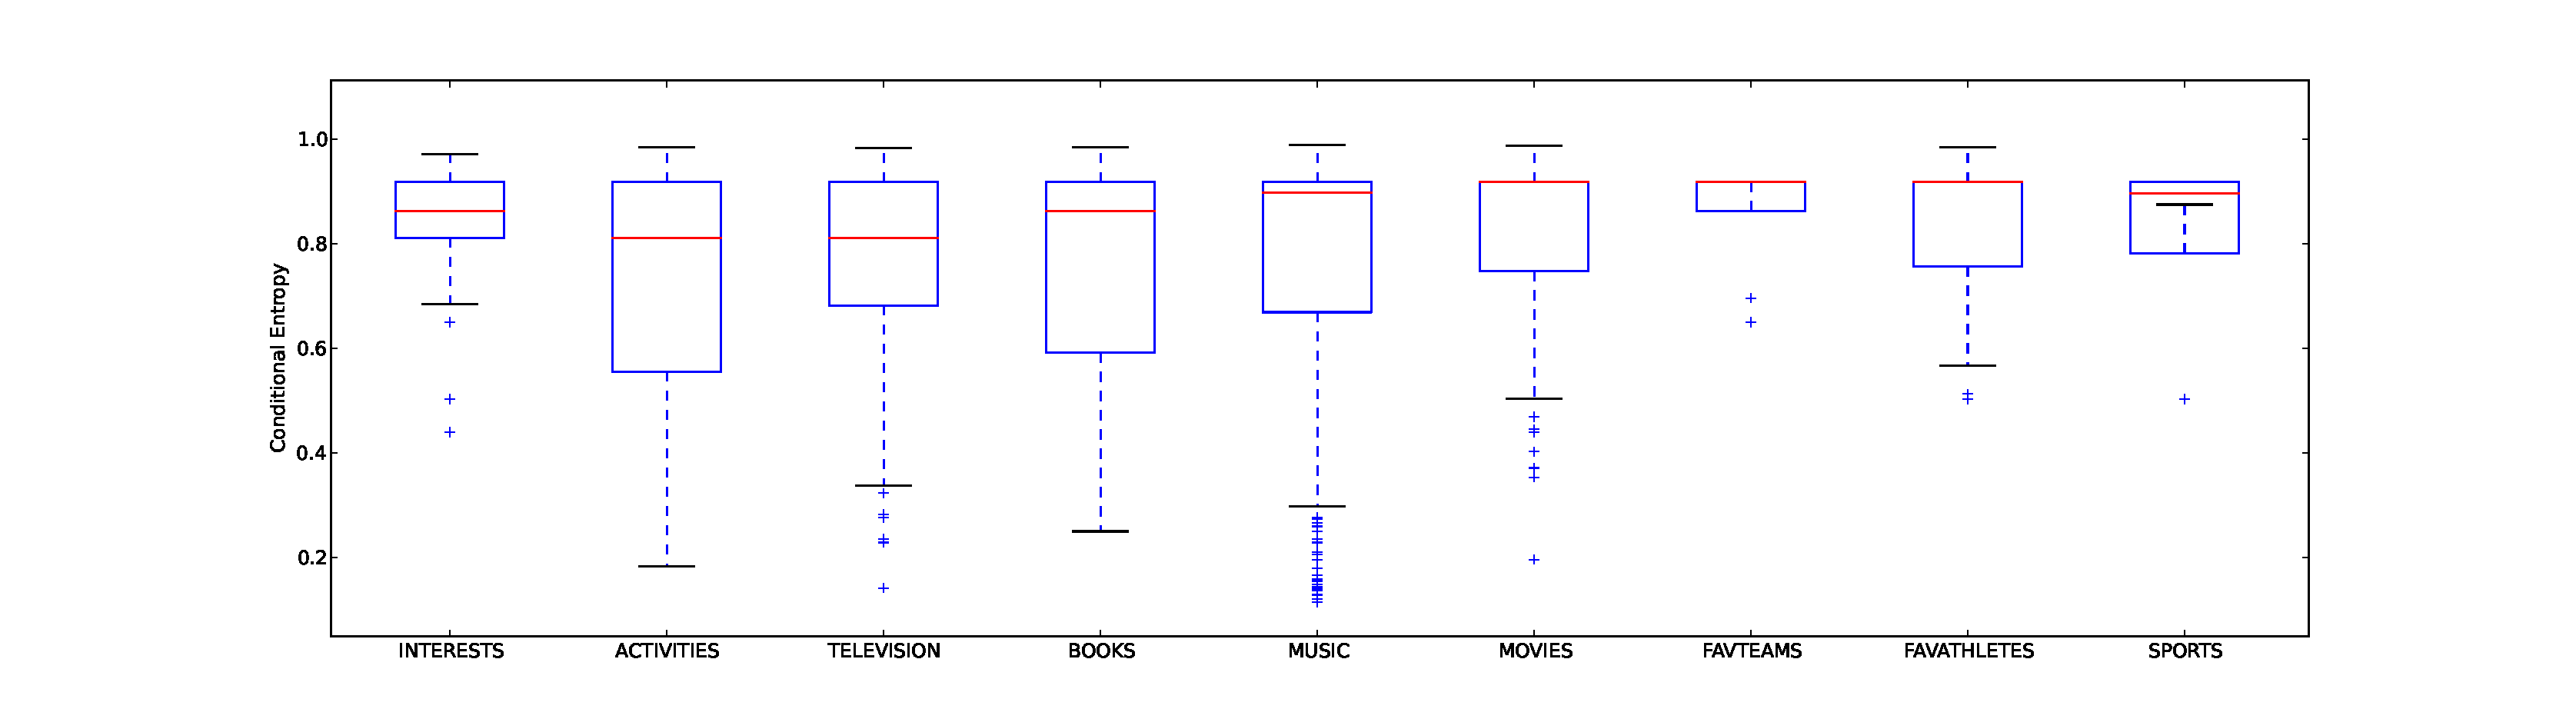
\includegraphics[height=40mm,width=150mm]{data/plots/boxPlots/CEvsFavTypes.eps}}\\
\subfloat[Fig:  mutual information vs favourite categories][mutual information vs favourite categories]{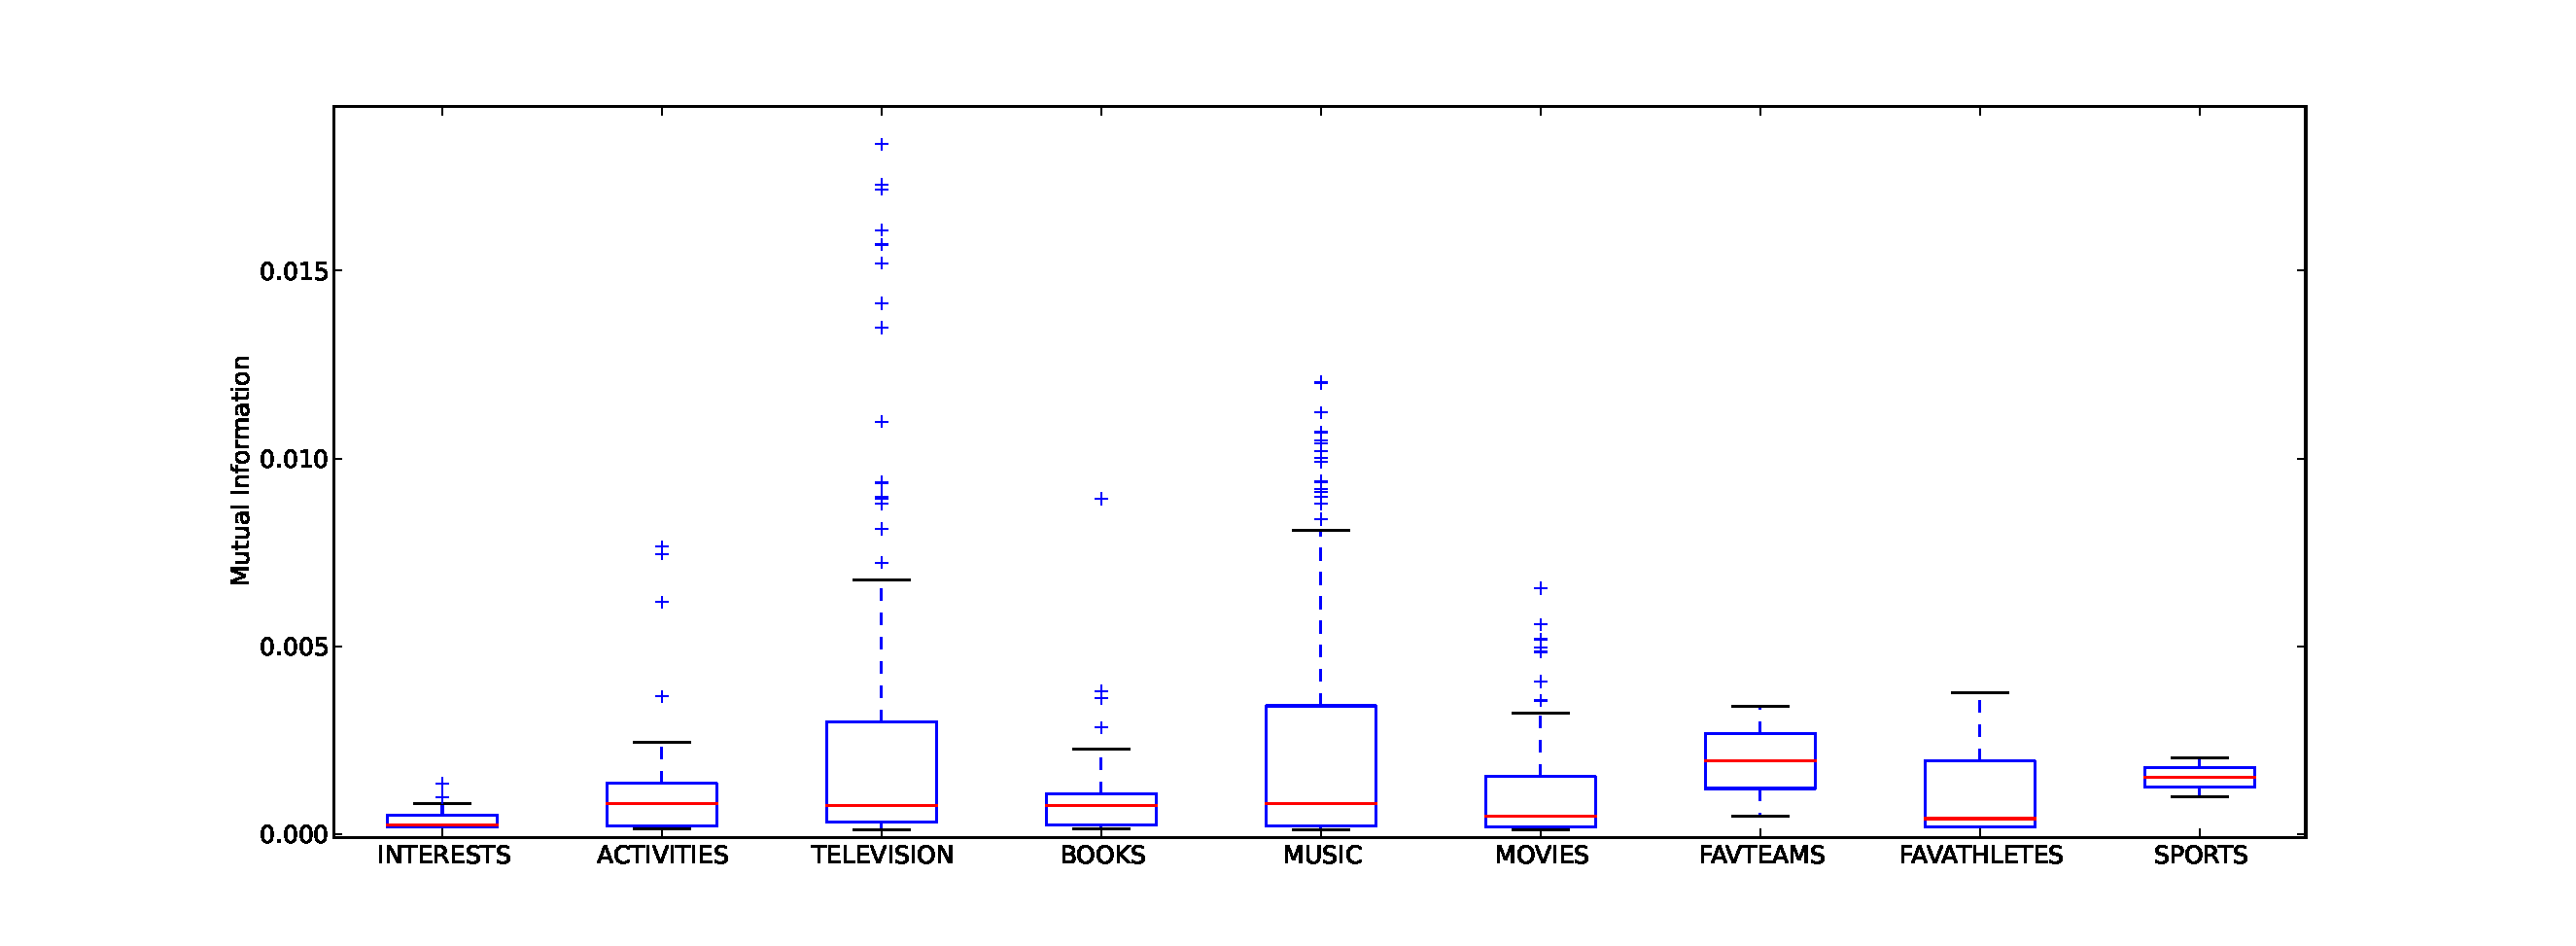
\includegraphics[height=40mm,width=150mm]{data/plots/boxPlots/MIvsFavTypes.eps}}
\end{tabular}
\caption{ mutual information  vs favourite categories}
\label{Fig: mutual information  vs favourite categories}
\end{figure*}


\begin{figure*}[h]
\centering
\begin{tabular}{ccc}
\subfloat[Fig: conditional entropy vs group size ][CE vs group]{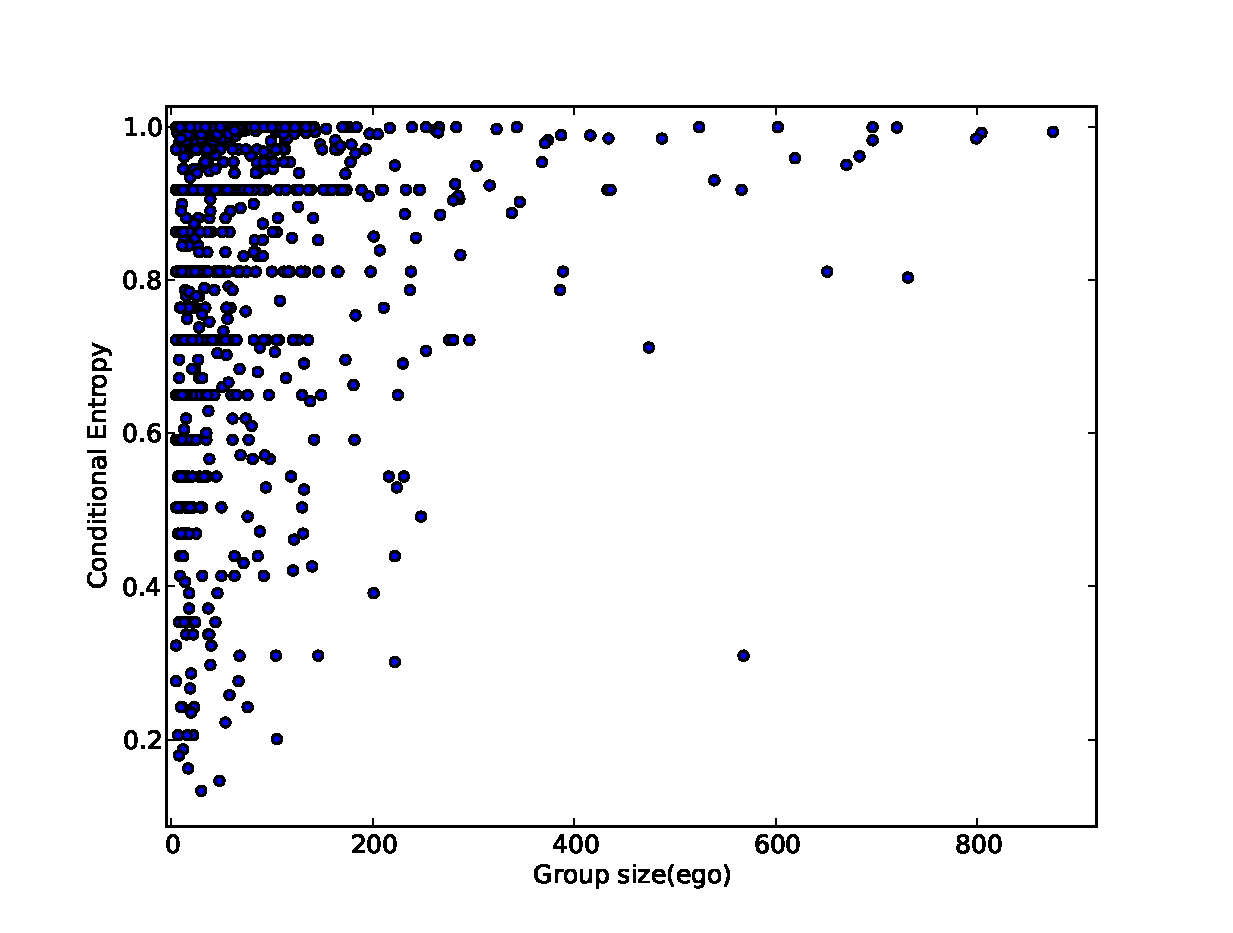
\includegraphics[width=40mm, height=30mm]{data/plots/scatterplots/vssize/CEvsGroupSizeEgo.eps}}
\subfloat[Fig: conditional entropy vs page size ][CE vs page]{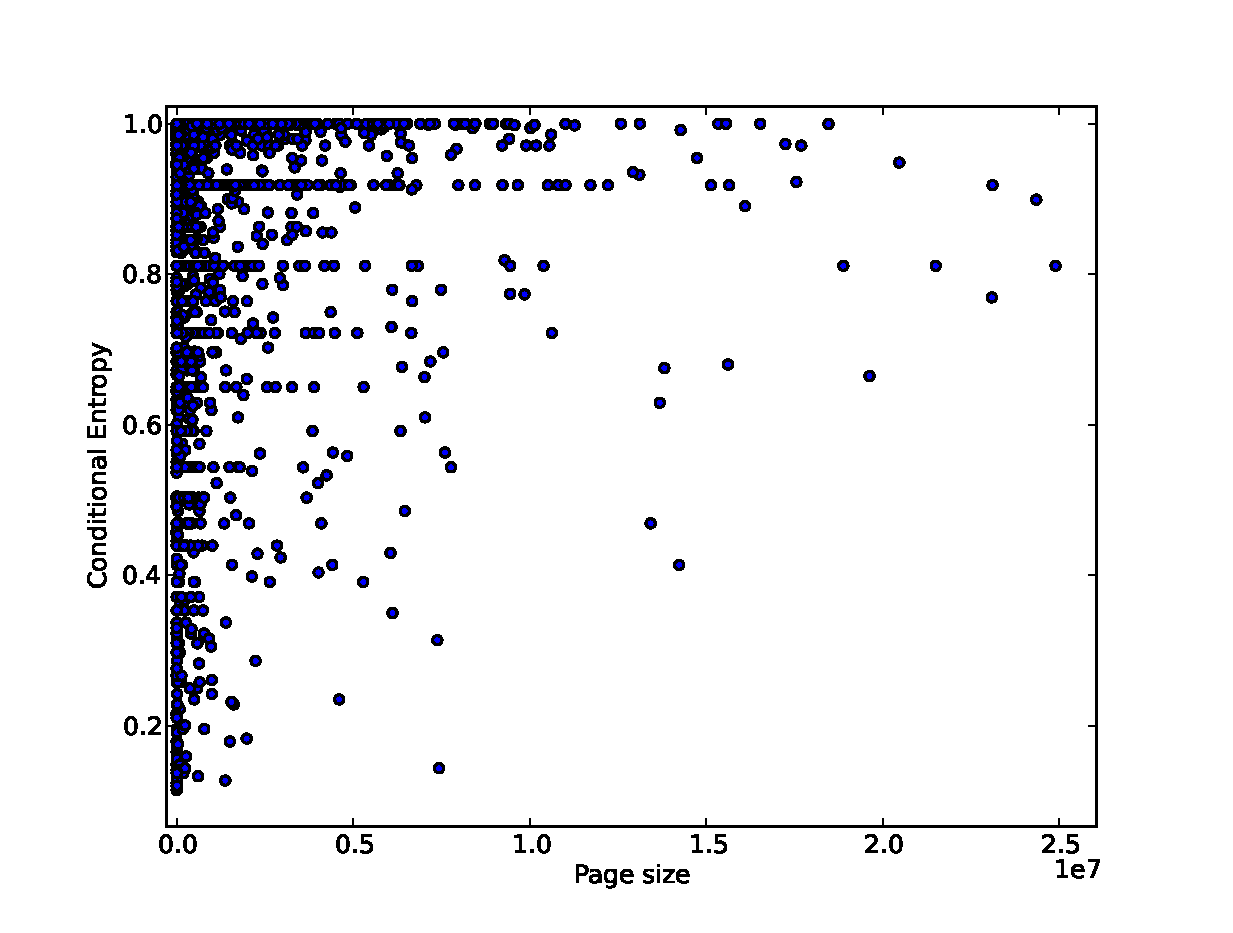
\includegraphics[width=40mm, height=30mm]{data/plots/scatterplots/vssize/CEvsPageSize.eps}}
\subfloat[Fig: conditional entropy vs favourite size ][CE vs favourite]{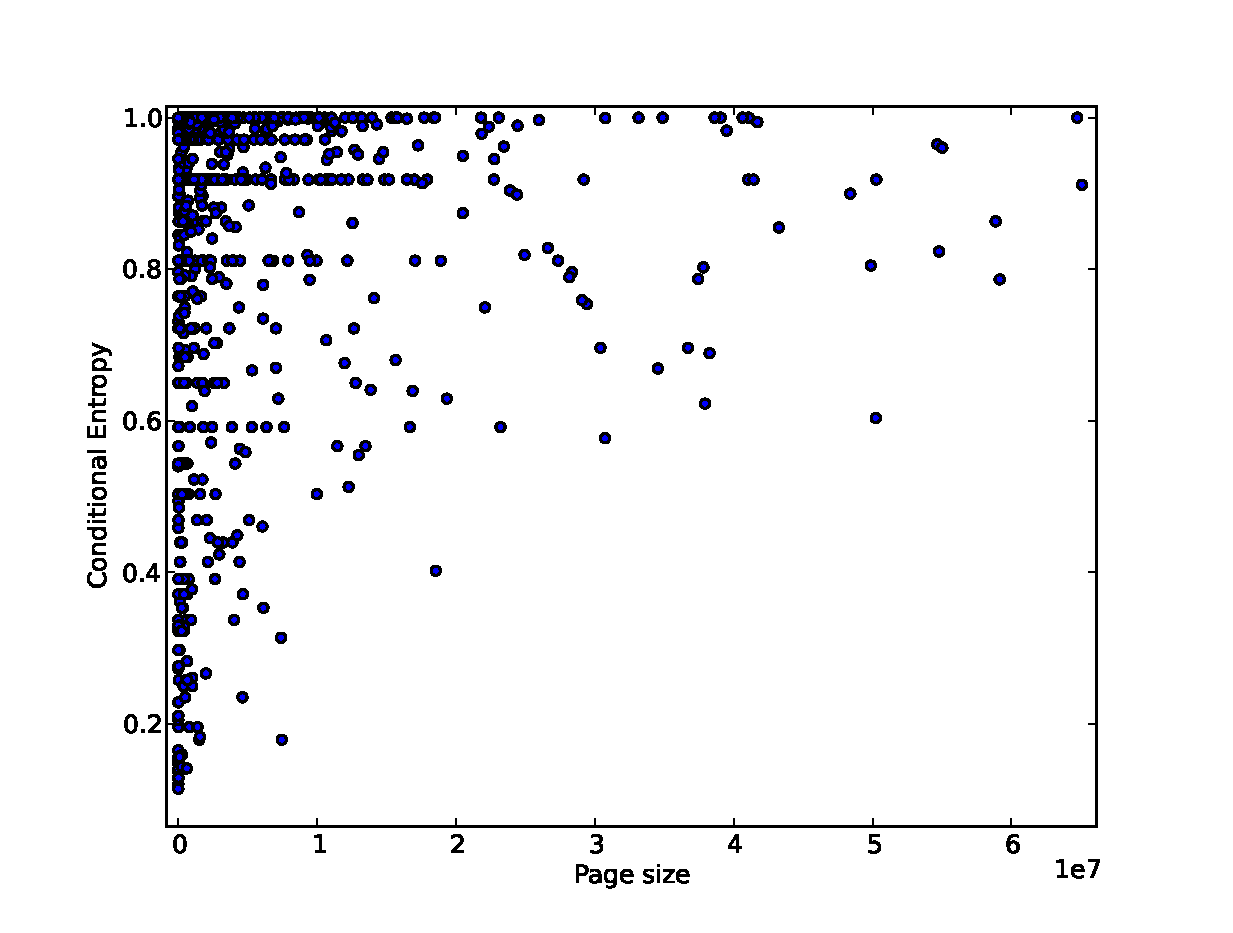
\includegraphics[width=40mm, height=30mm]{data/plots/scatterplots/vssize/CEvsFavSize.eps}} \\
\subfloat[Fig: conditional entropy vs group size(log) ][CE vs group]{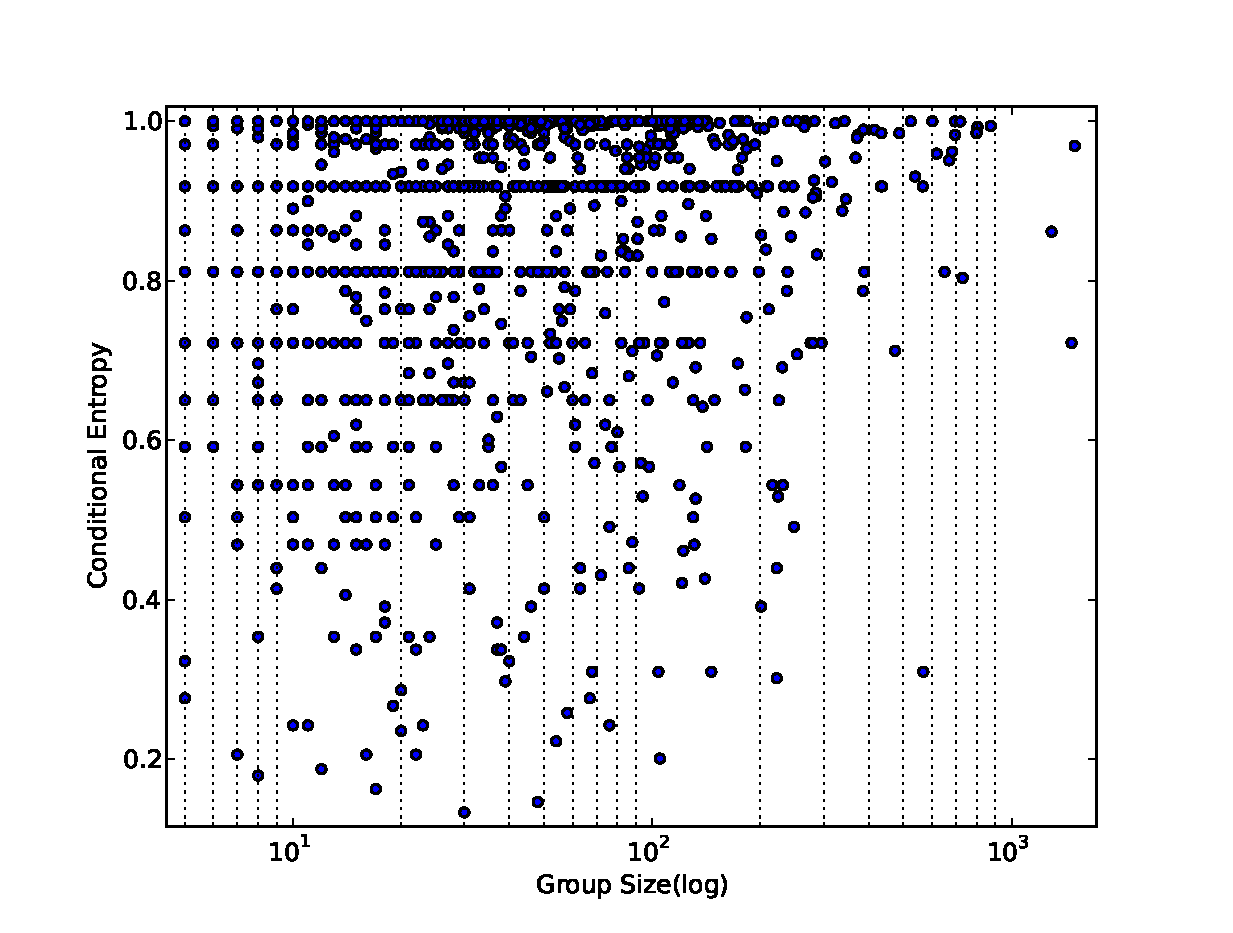
\includegraphics[width=40mm, height=30mm]{data/plots/scatterplots/vssize/CEvsGroupSizeLog.eps}}
\subfloat[Fig: conditional entropy vs page size(log) ][CE vs page]{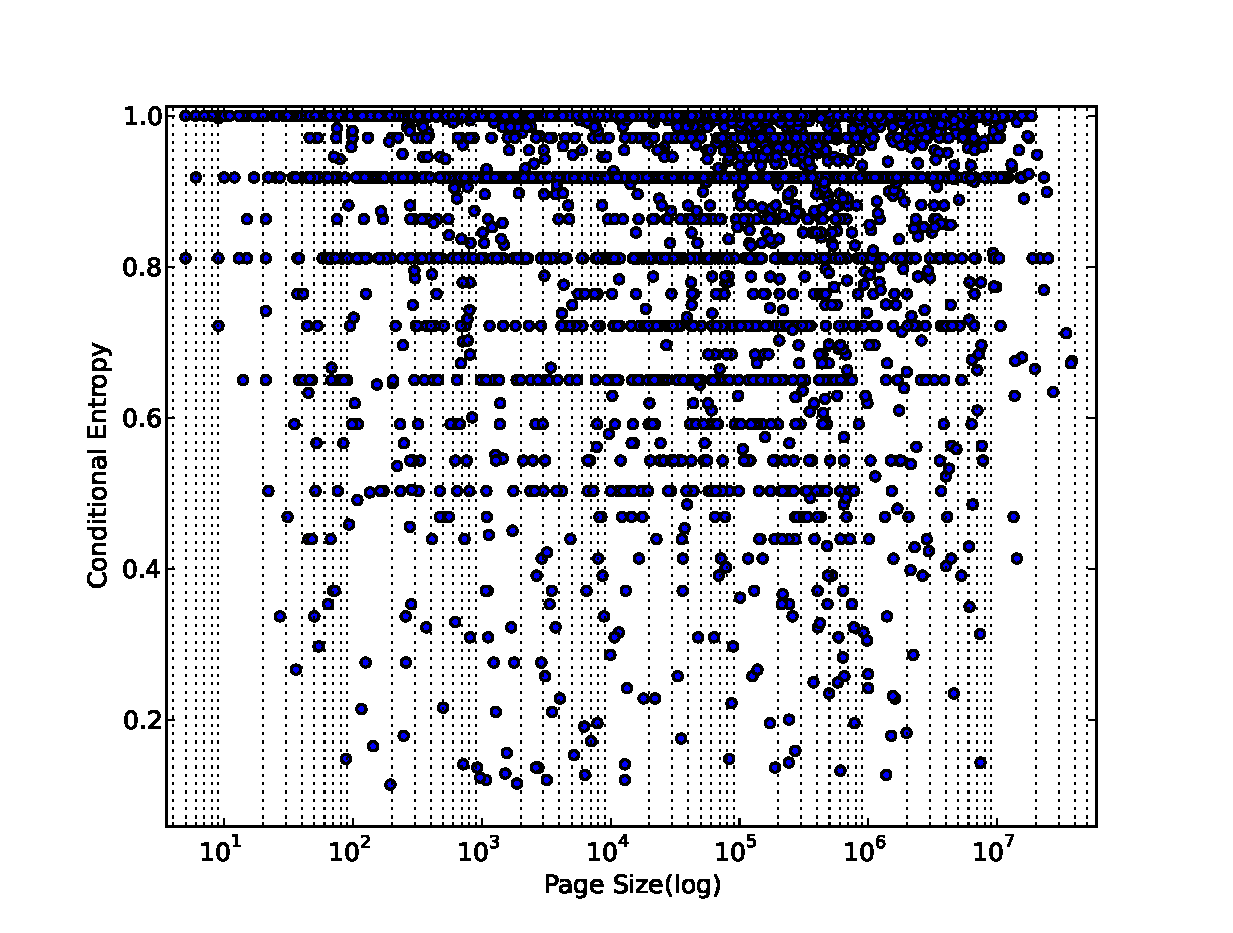
\includegraphics[width=40mm, height=30mm]{data/plots/scatterplots/vssize/CEvsPageSizeLog.eps}}
\subfloat[Fig: conditional entropy vs favourite size(log) ][CE vs favourite]{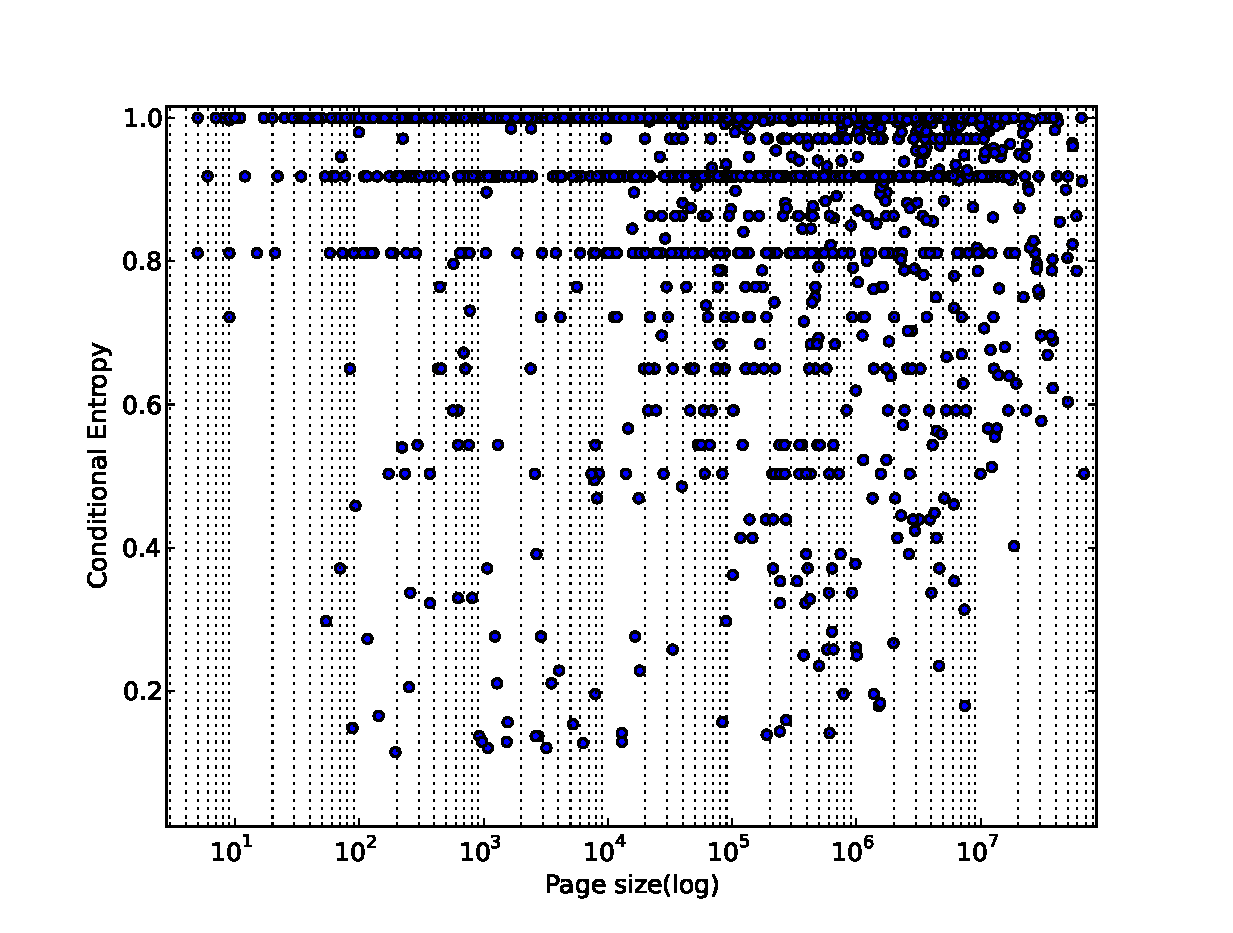
\includegraphics[width=40mm, height=30mm]{data/plots/scatterplots/vssize/CEvsFavSizeLog.eps}}\\
\subfloat[Fig: conditional entropy vs group size(ego) ][CE vs group(ego)]{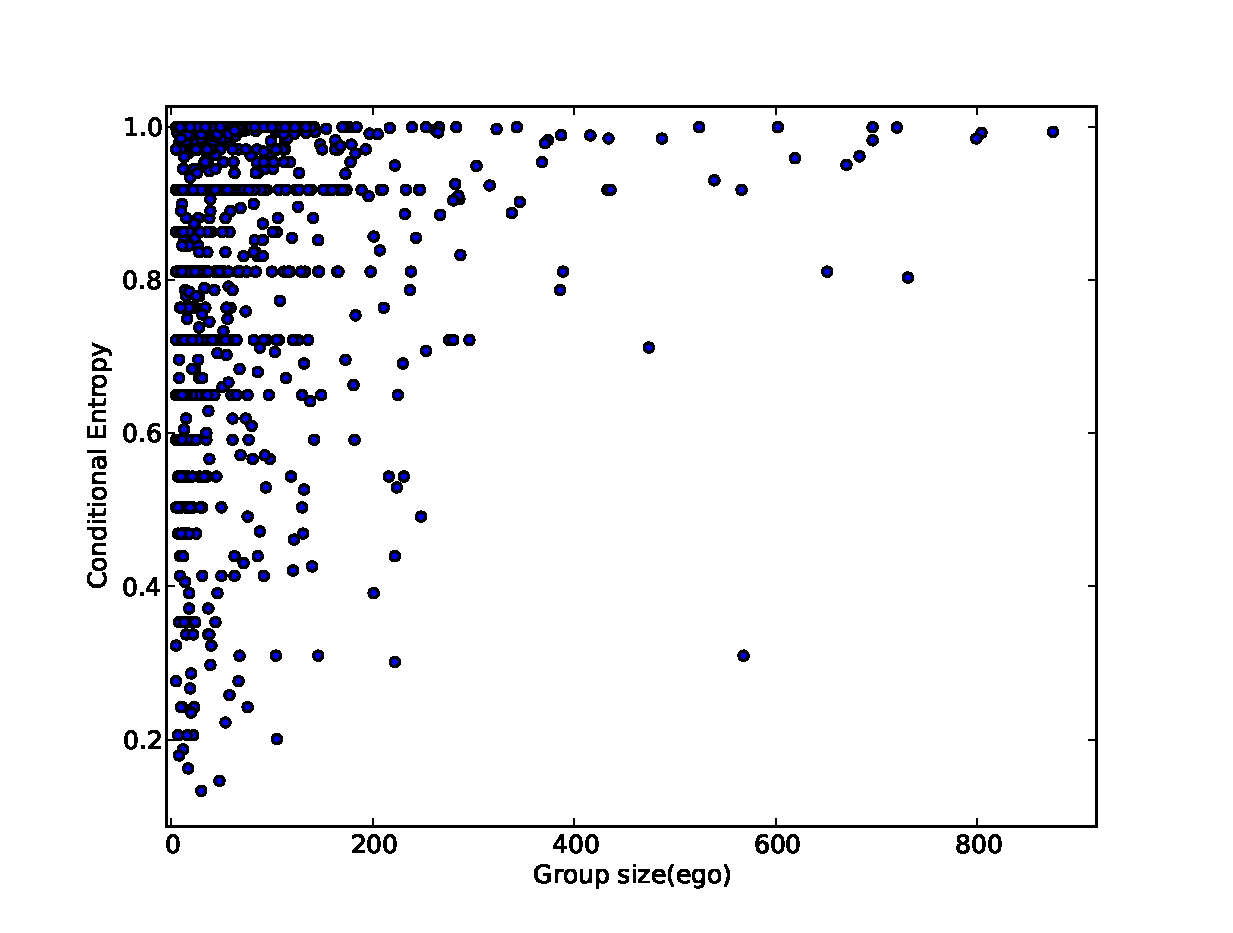
\includegraphics[width=40mm, height=30mm]{data/plots/scatterplots/vssize/CEvsGroupSizeEgo.eps}}
\subfloat[Fig: conditional entropy vs page size ][CE vs page(ego)]{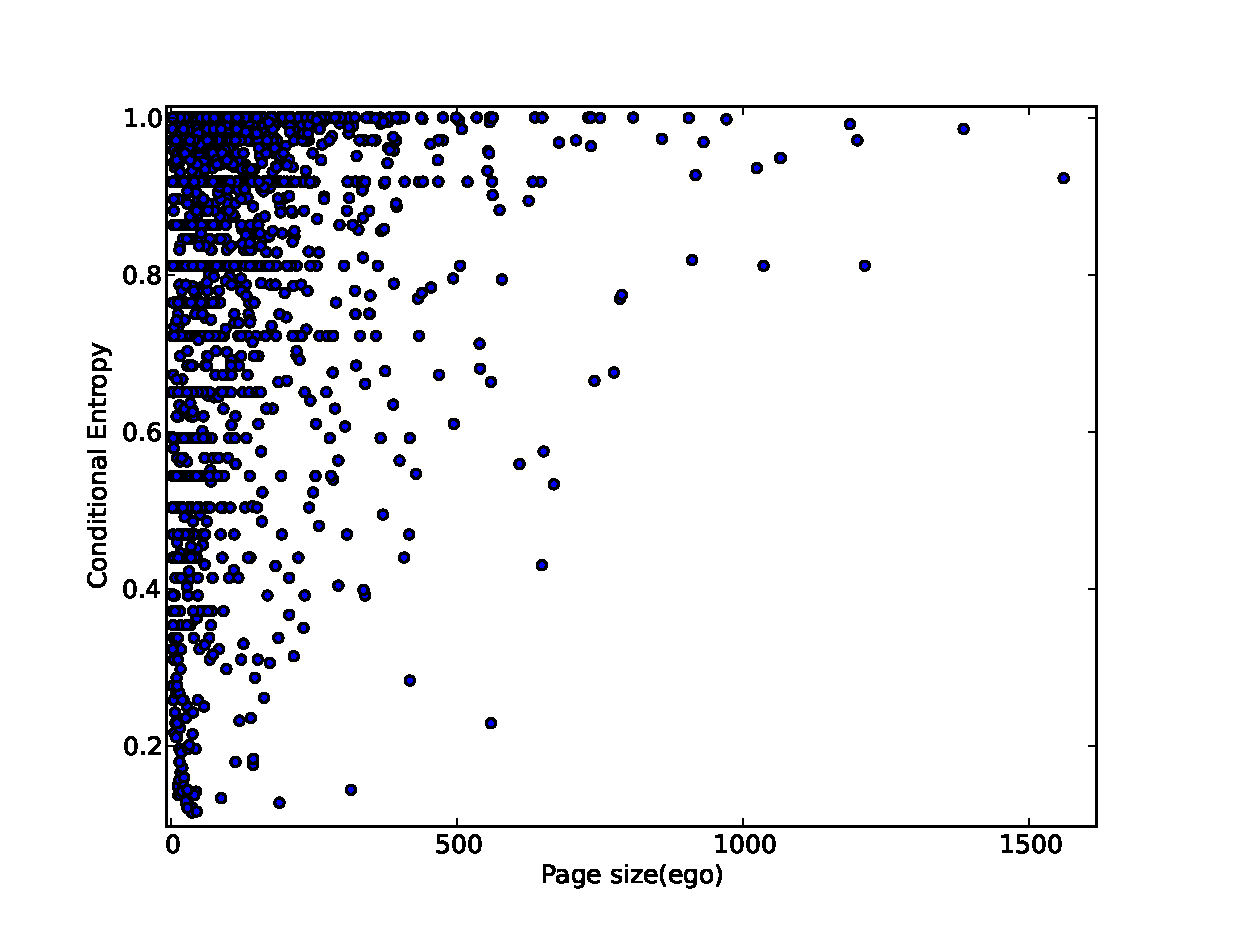
\includegraphics[width=40mm, height=30mm]{data/plots/scatterplots/vssize/CEvsPageSizeEgo.eps}}
\subfloat[Fig: conditional entropy vs favourite size(ego) ][CE vs favourite(ego)]{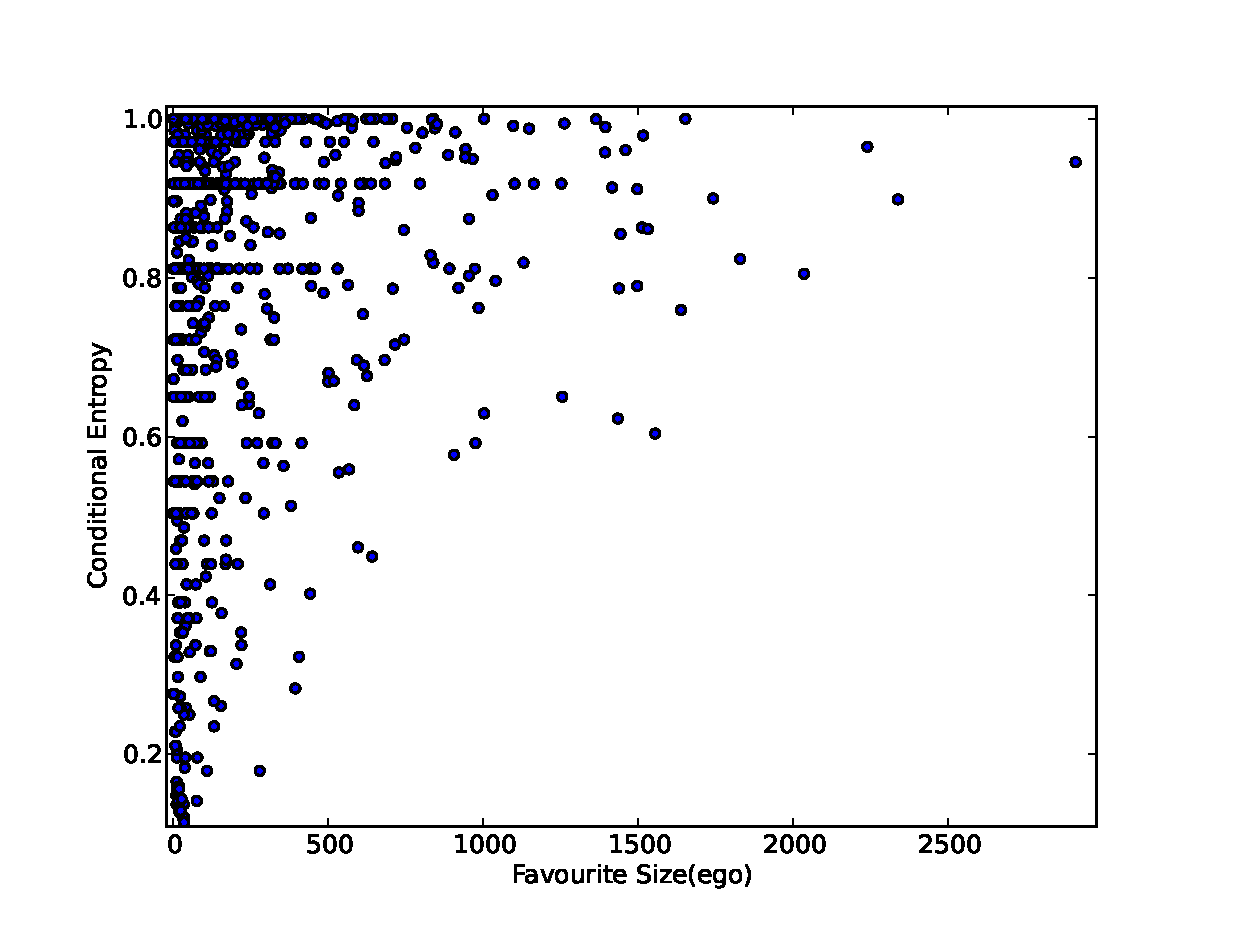
\includegraphics[width=40mm, height=30mm]{data/plots/scatterplots/vssize/CEvsFavSizeEgo.eps}}
\end{tabular}
\caption{conditional entropy vs size}
\label{Fig: conditional entropy vs size}
\end{figure*}

\begin{figure*}[h]
\centering
\begin{tabular}{ccc}
\subfloat[Fig: mutual information vs group size ][MI vs group]{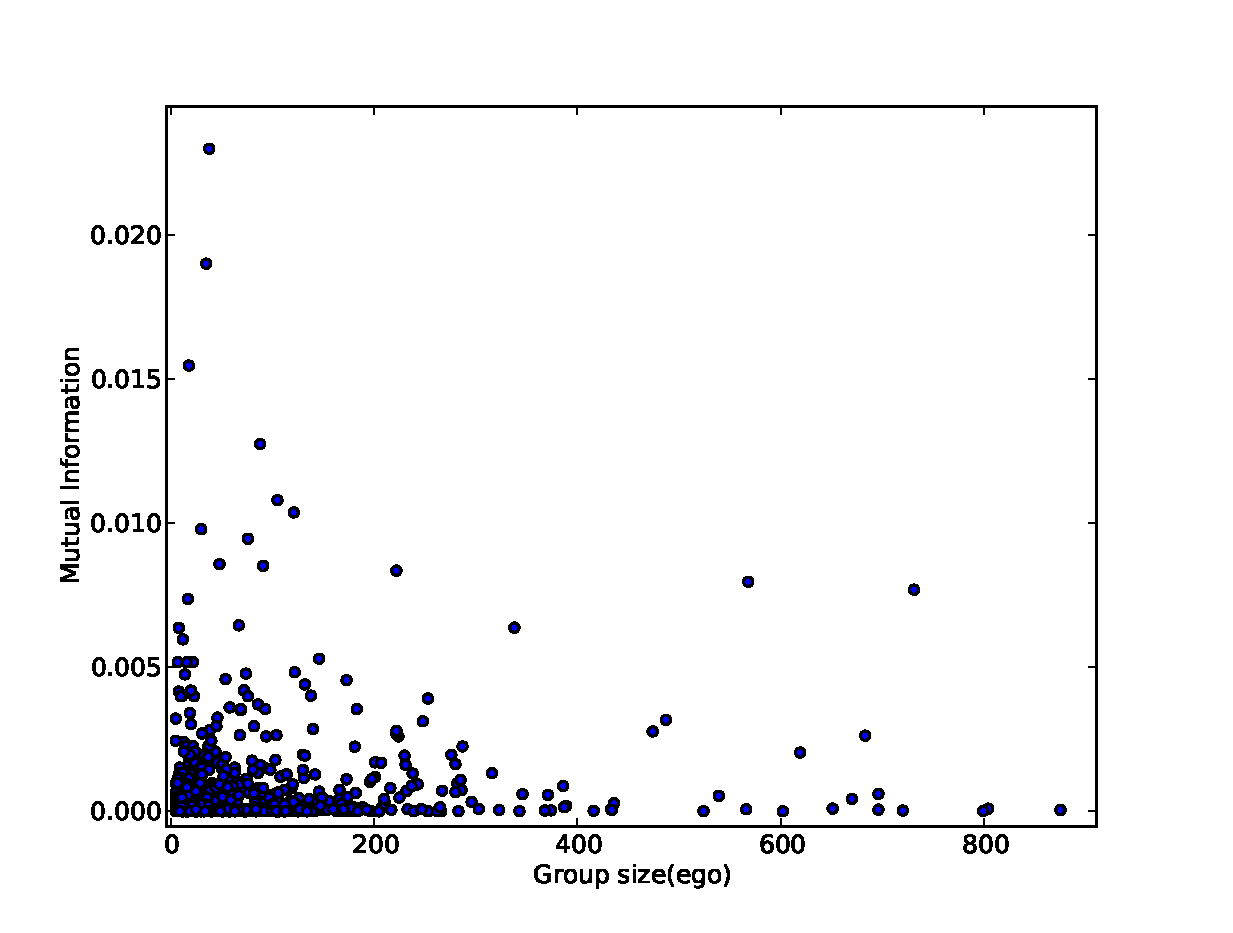
\includegraphics[width=40mm, height=30mm]{data/plots/scatterplots/vssize/MIvsGroupSizeEgo.eps}}
\subfloat[Fig: mutual information vs page size ][MI vs page]{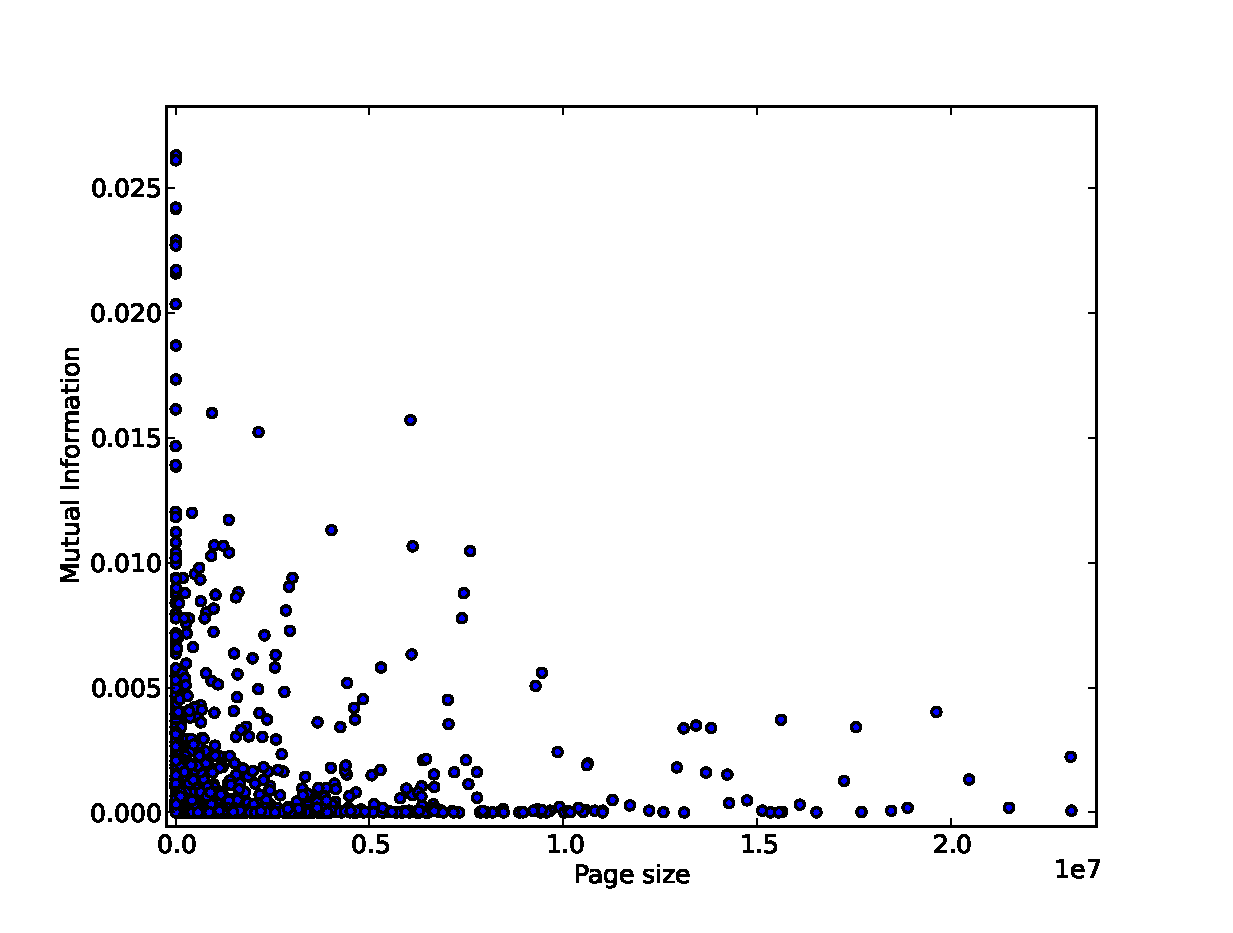
\includegraphics[width=40mm, height=30mm]{data/plots/scatterplots/vssize/MIvsPageSize.eps}}
\subfloat[Fig: mutual information vs favourite size ][MI vs favourite]{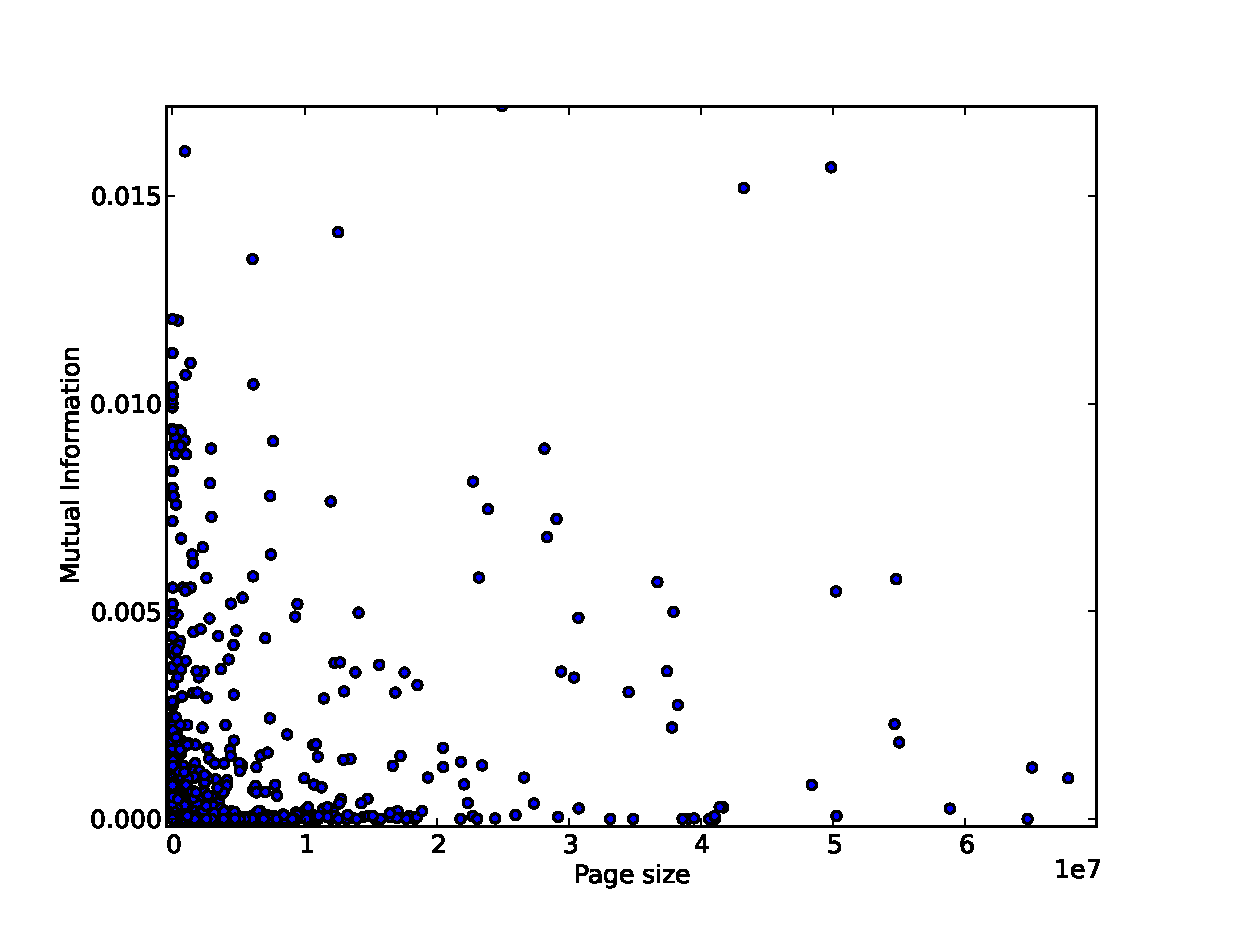
\includegraphics[width=40mm, height=30mm]{data/plots/scatterplots/vssize/MIvsFavSize.eps}} \\
\subfloat[Fig: mutual information vs group size(log) ][MI vs group]{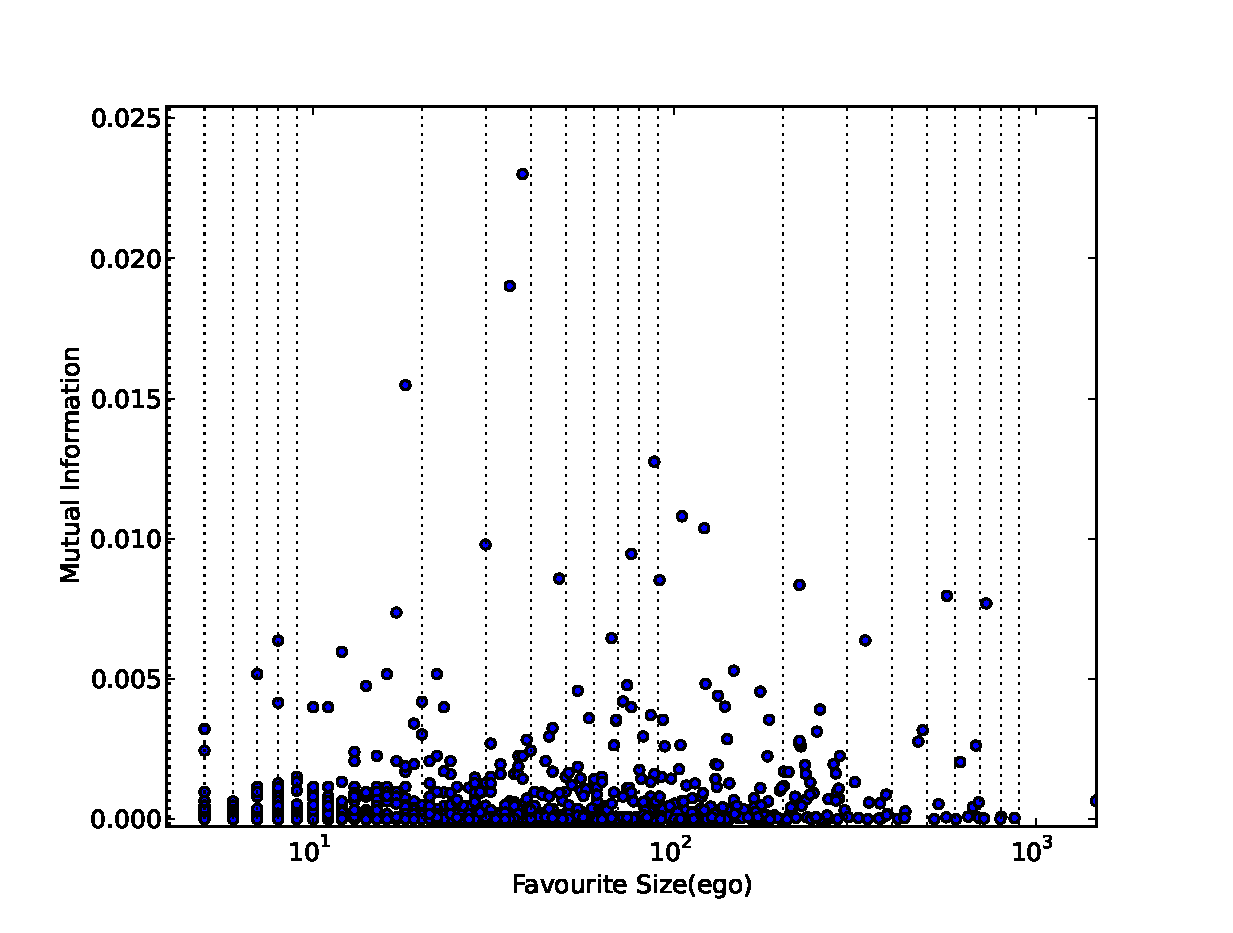
\includegraphics[width=40mm, height=30mm]{data/plots/scatterplots/vssize/MIvsGroupSizeLog.eps}}
\subfloat[Fig: mutual information vs page size(log) ][MI vs page]{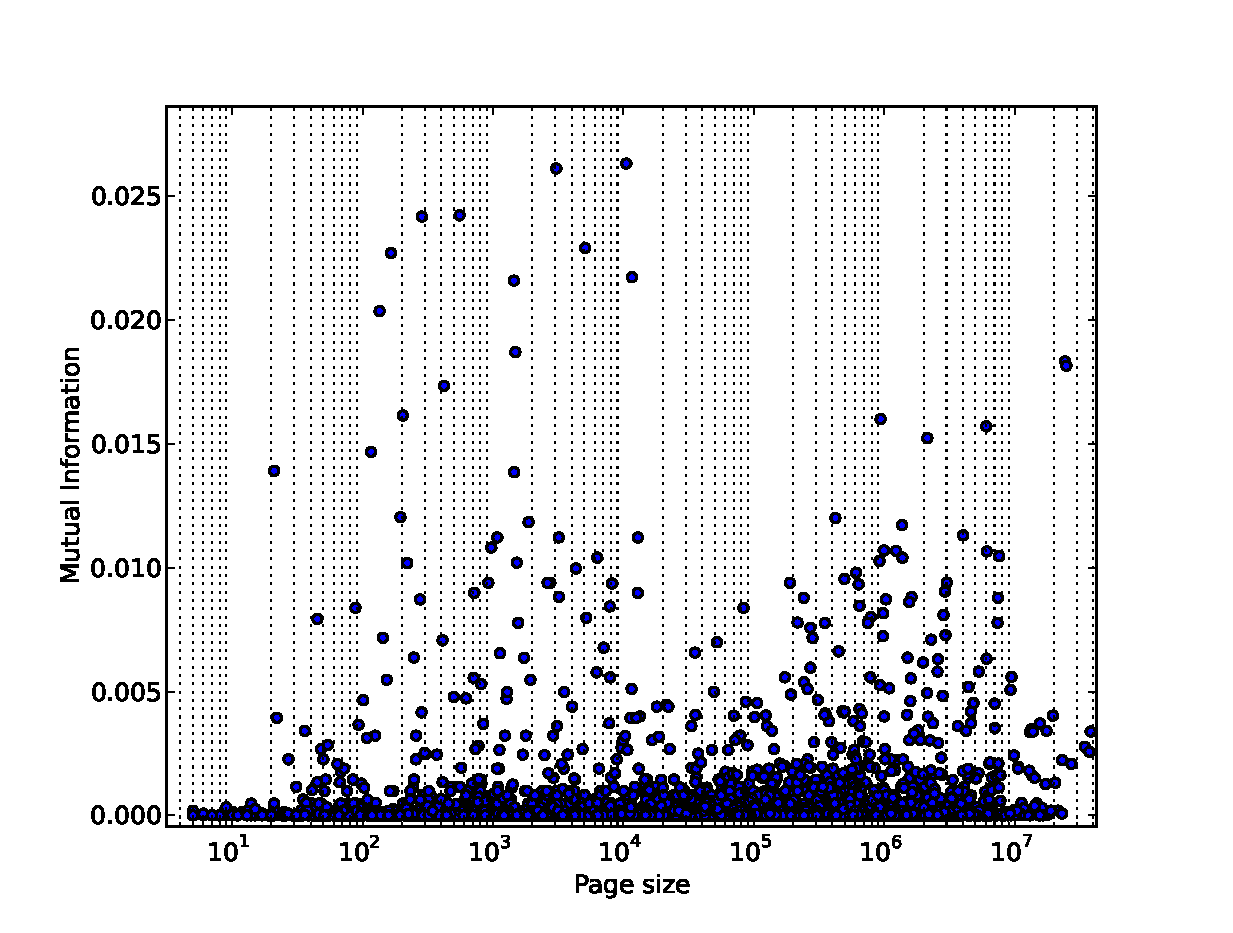
\includegraphics[width=40mm, height=30mm]{data/plots/scatterplots/vssize/MIvsPageSizeLog.eps}}
\subfloat[Fig: mutual information vs favourite size(log) ][MI vs favourite]{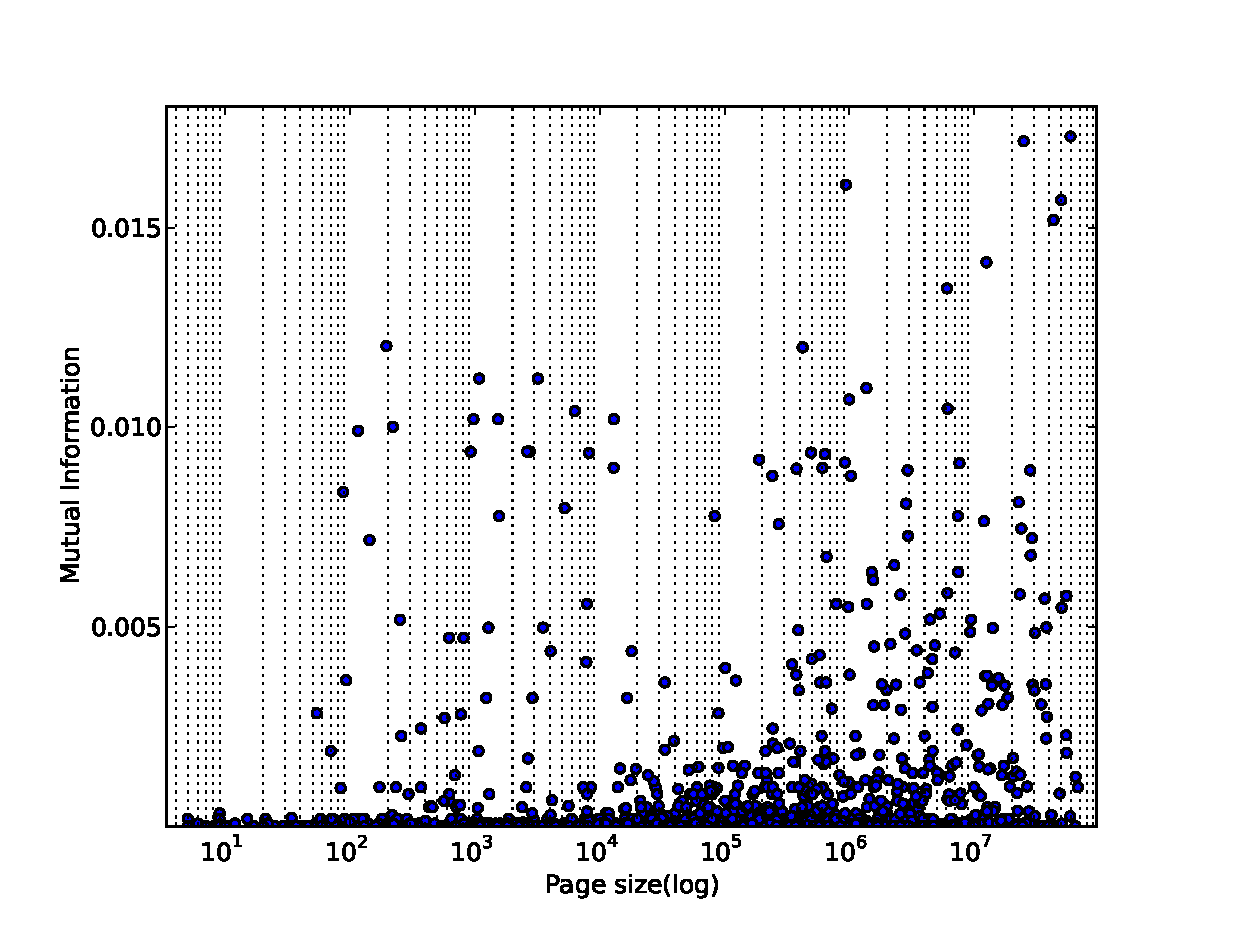
\includegraphics[width=40mm, height=30mm]{data/plots/scatterplots/vssize/MIvsFavSizeLog.eps}}\\
\subfloat[Fig: mutual information vs group size(ego) ][MI vs group(ego)]{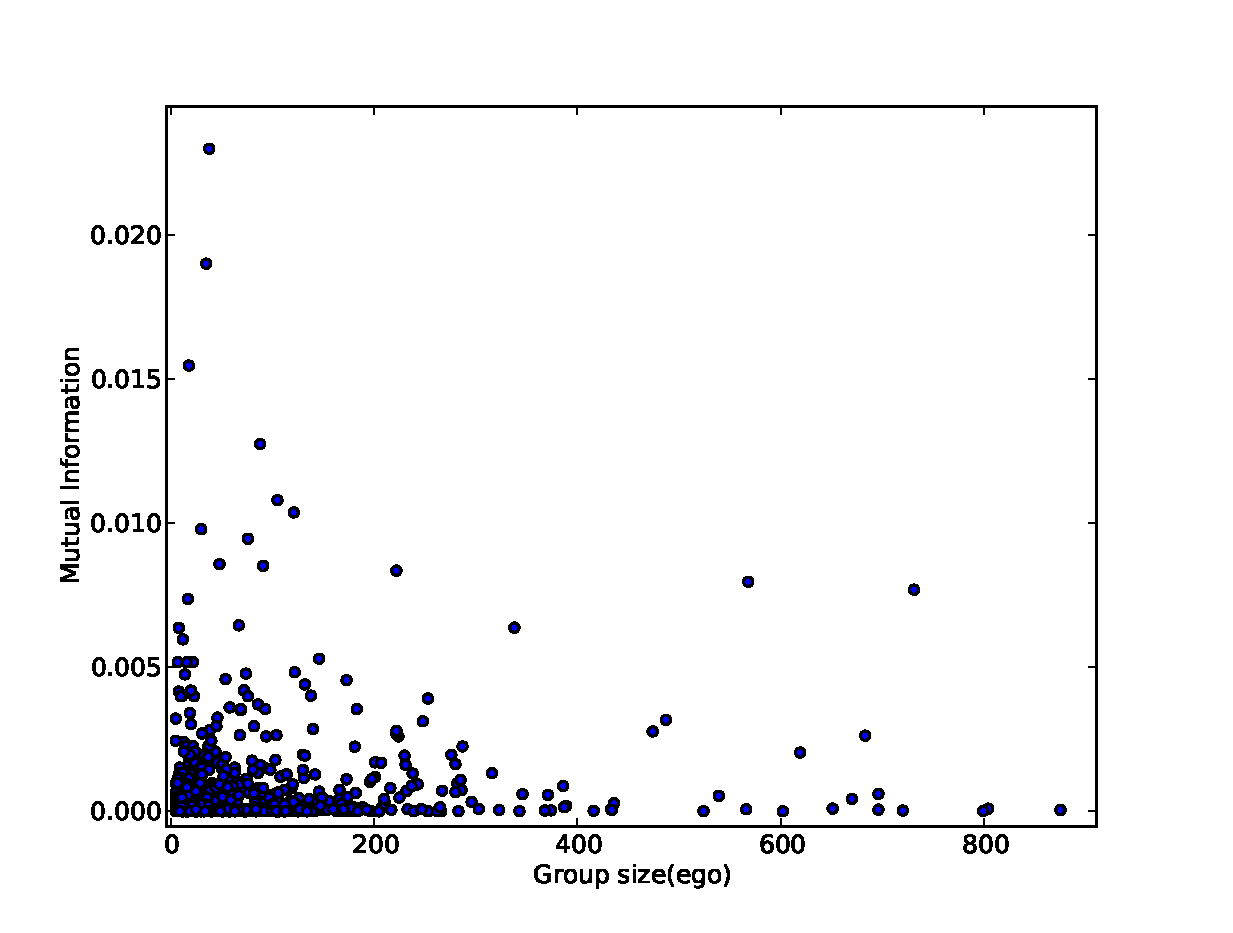
\includegraphics[width=40mm, height=30mm]{data/plots/scatterplots/vssize/MIvsGroupSizeEgo.eps}}
\subfloat[Fig: mutual information vs page size ][MI vs page(ego)]{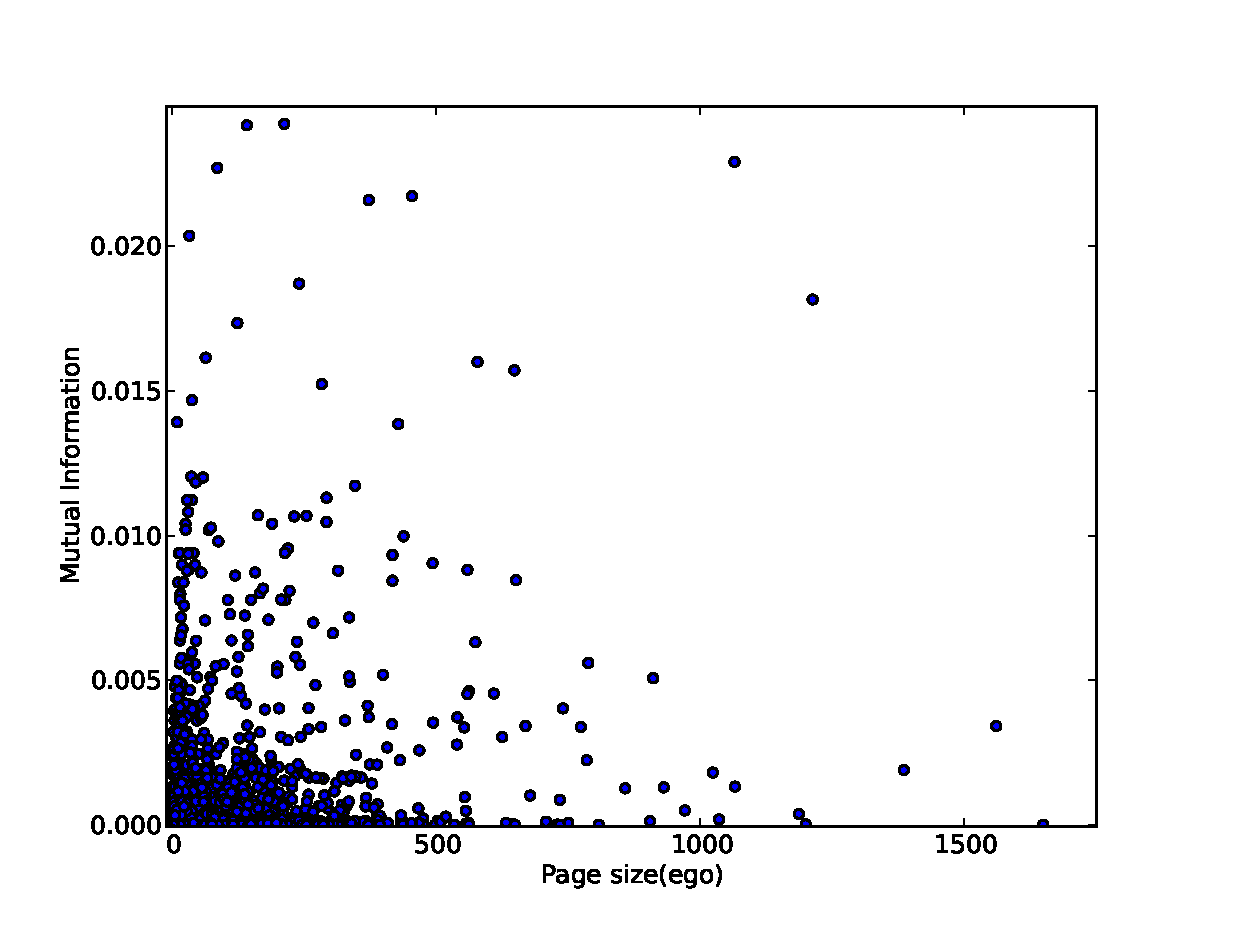
\includegraphics[width=40mm, height=30mm]{data/plots/scatterplots/vssize/MIvsPageSizeEgo.eps}}
\subfloat[Fig: mutual information vs favourite size(ego) ][MI vs favourite(ego)]{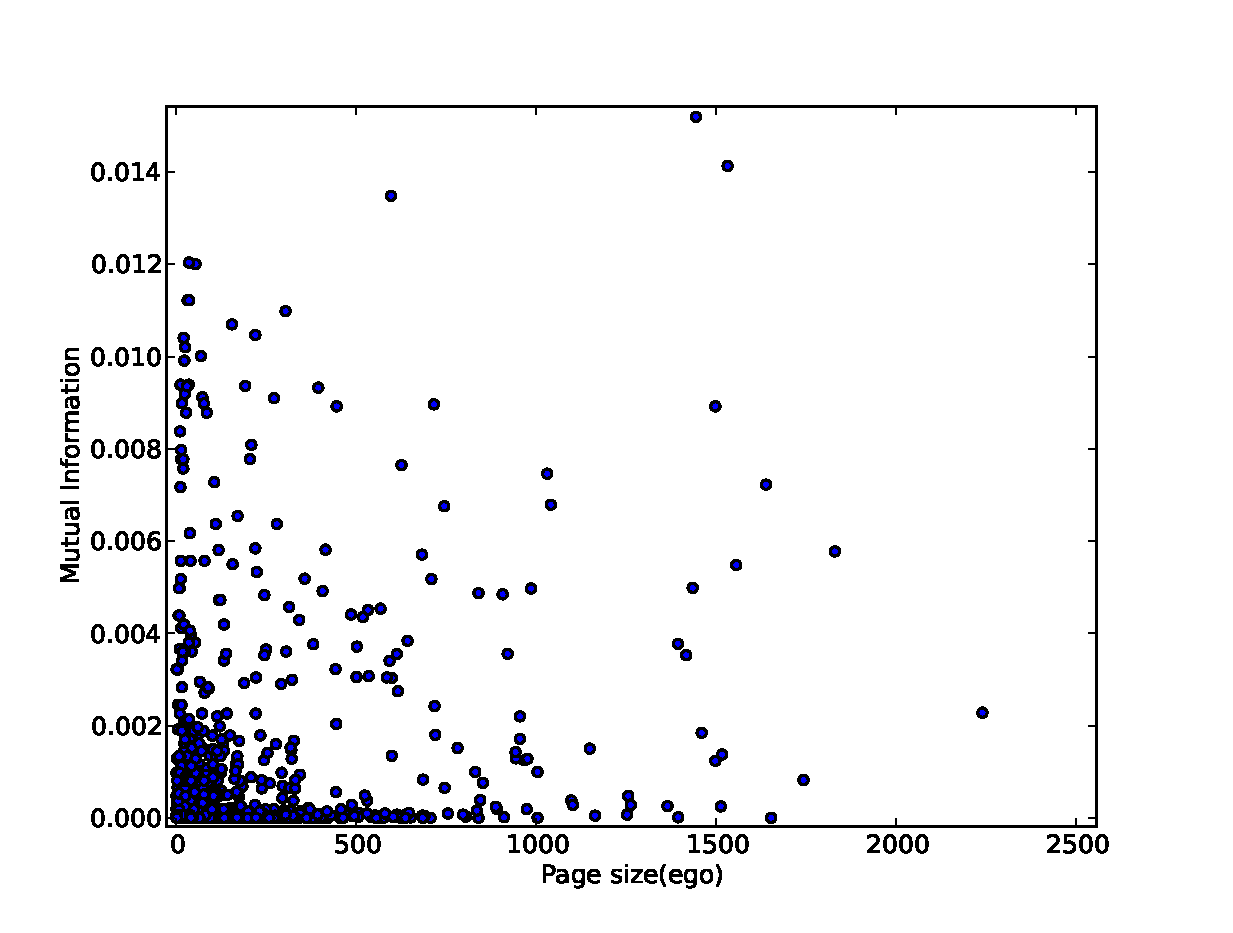
\includegraphics[width=40mm, height=30mm]{data/plots/scatterplots/vssize/MIvsFavSizeEgo.eps}}
\end{tabular}
\caption{ mutual information  vs size}
\label{Fig: mutual information  vs size}
\end{figure*}


\begin{figure*}[h]
\centering
\begin{tabular}{ccc}
\subfloat[Fig: logistic regression coefficients vs group size ][LR coefficient vs group]{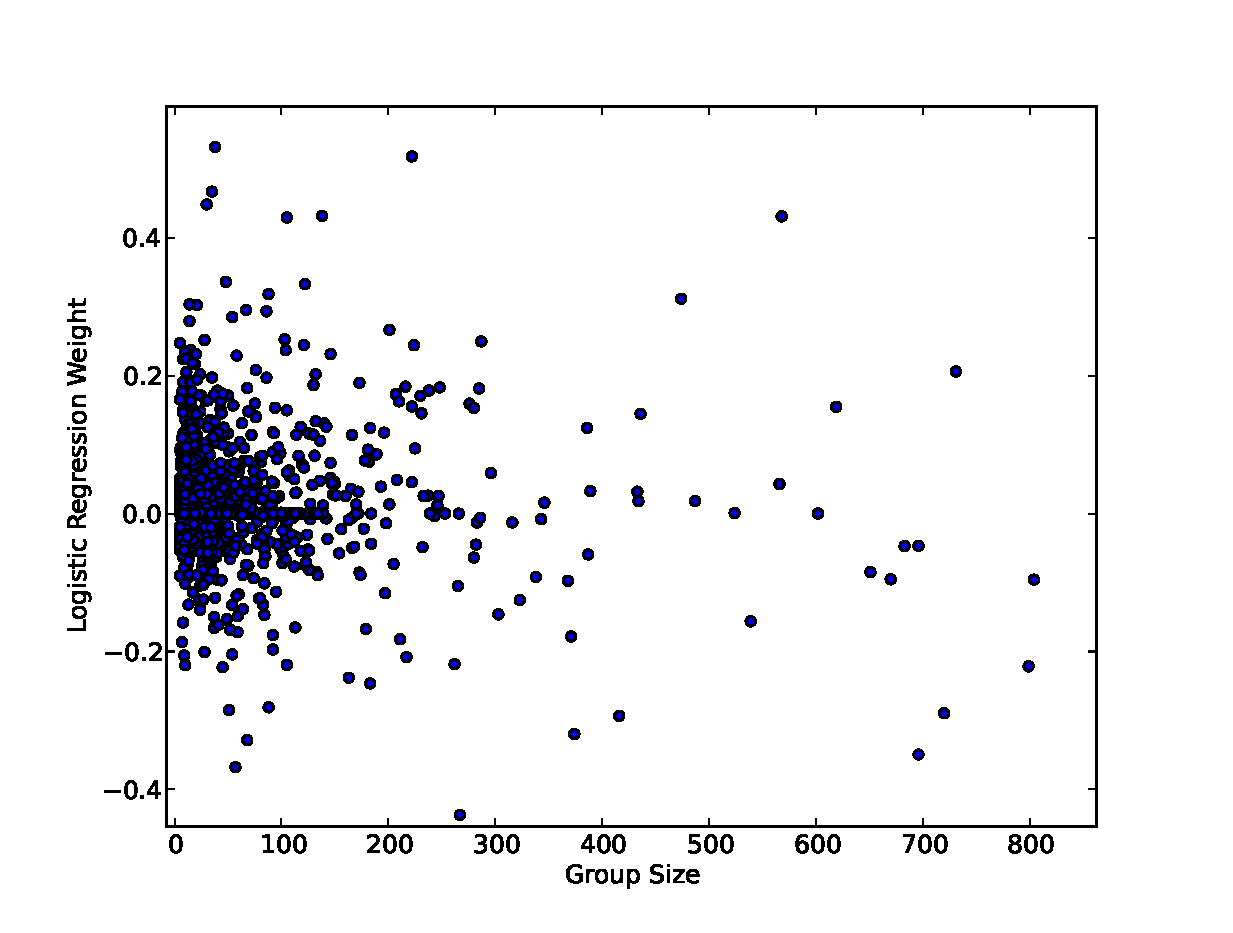
\includegraphics[width=40mm, height=30mm]{data/plots/scatterplots/LRweights/LRweightvsGroupSize.eps}}
\subfloat[Fig: logistic regression coefficients vs page size ][LR coefficient vs page]{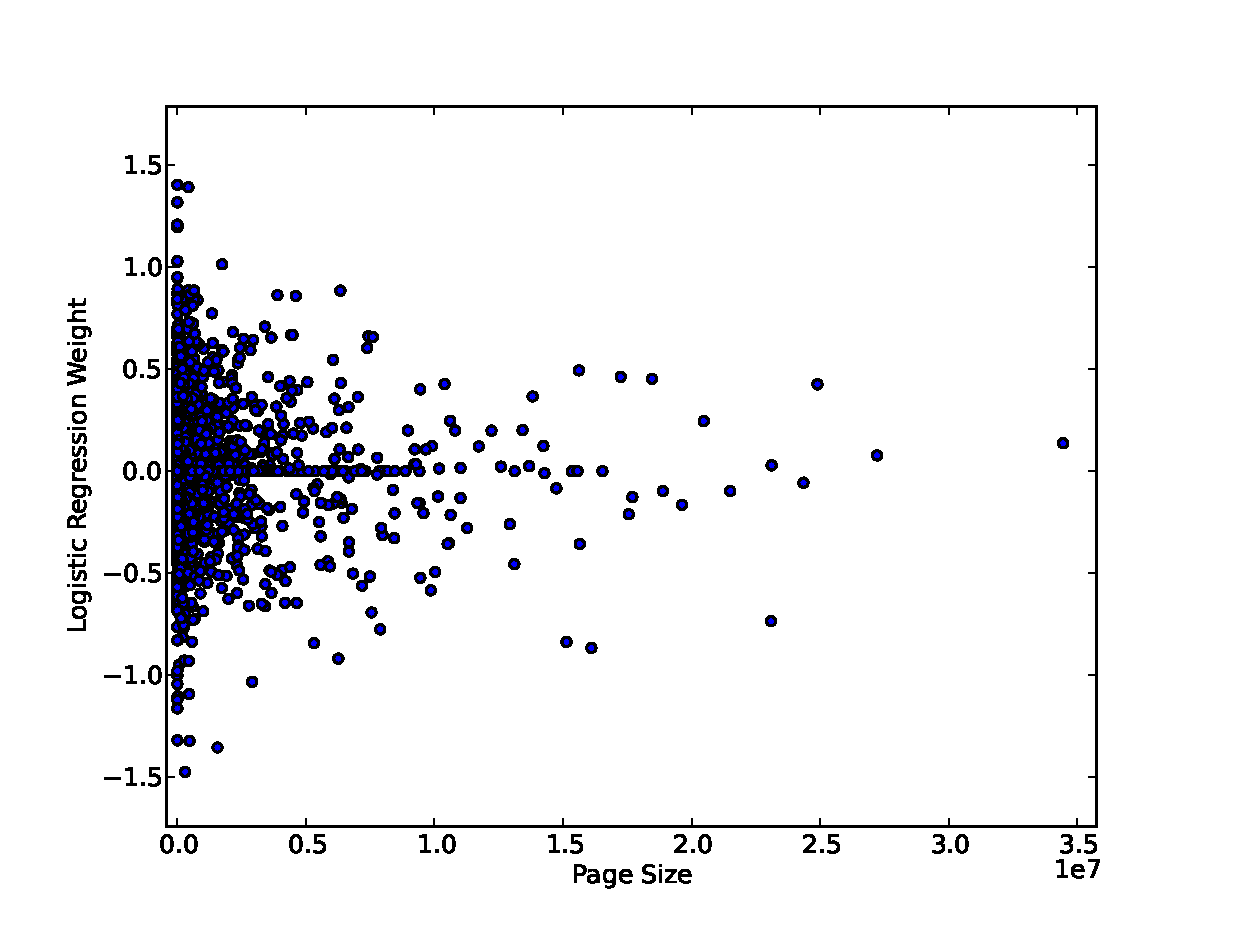
\includegraphics[width=40mm, height=30mm]{data/plots/scatterplots/LRweights/LRweightvsPageSize.eps}}
\subfloat[Fig: logistic regression coefficients vs favourite size ][LR coefficient vs favourite]{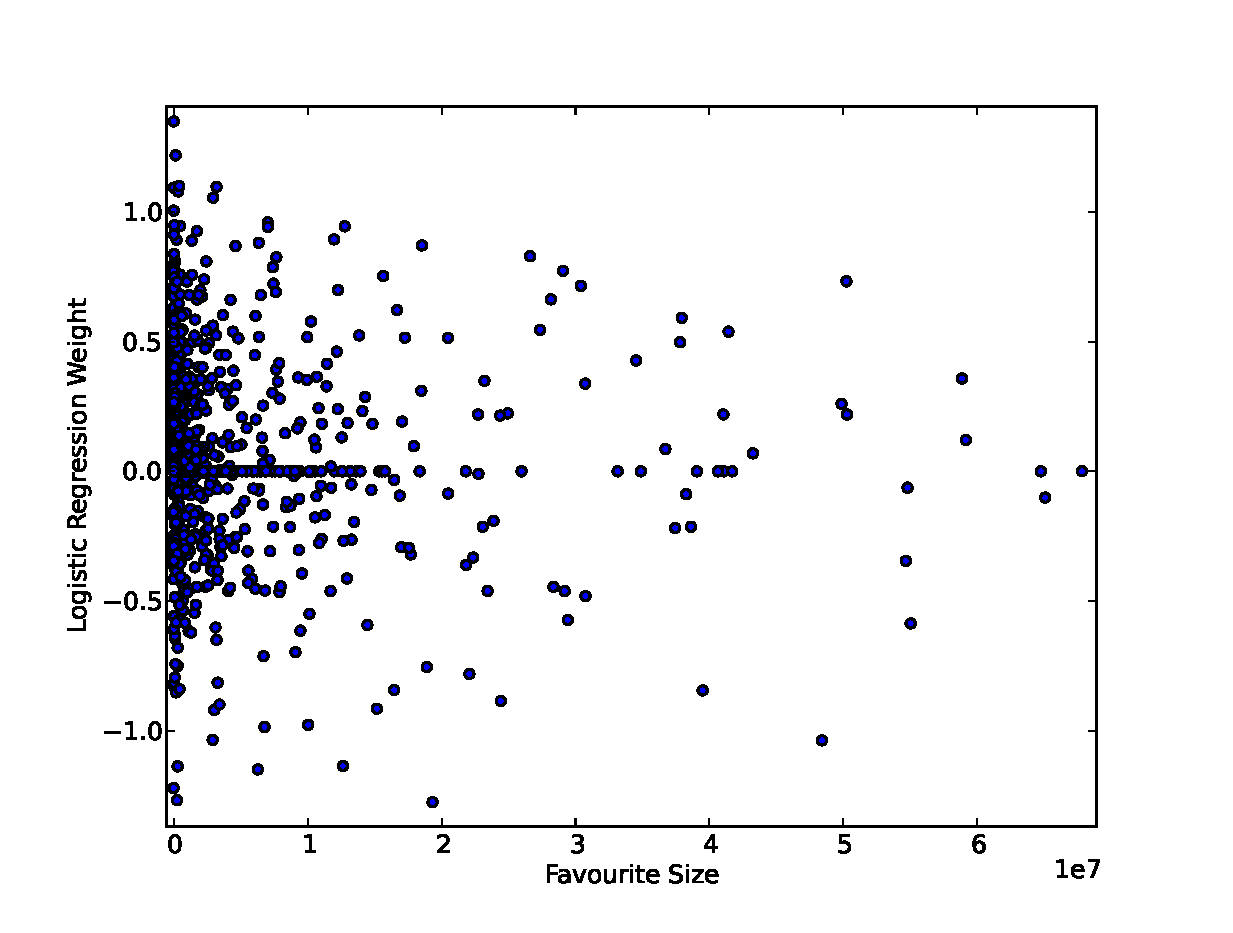
\includegraphics[width=40mm, height=30mm]{data/plots/scatterplots/LRweights/LRweightvsFavouriteSize.eps}} \\
\subfloat[Fig: logistic regression coefficients vs group size(ego) ][LR coefficient vs group(ego)]{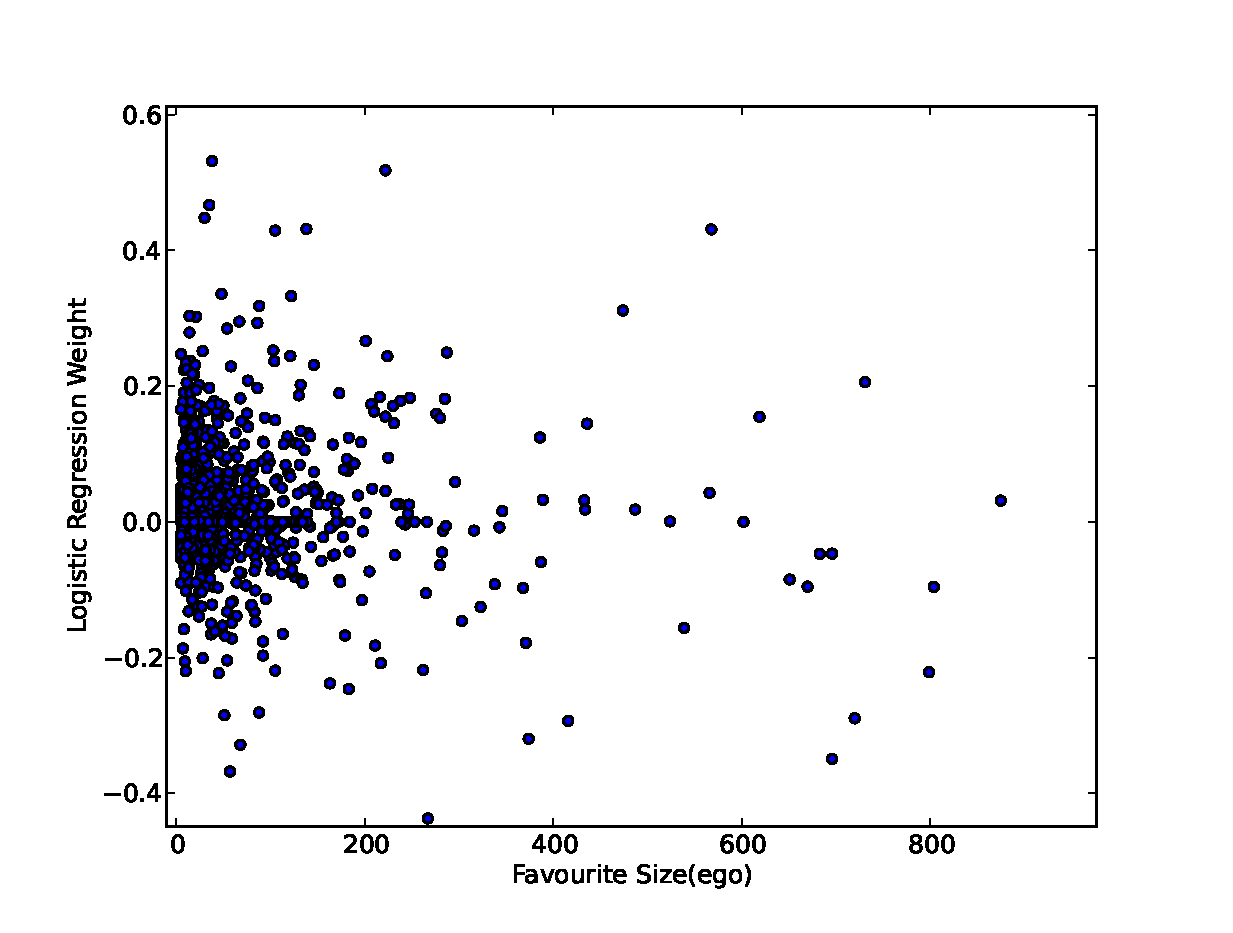
\includegraphics[width=40mm, height=30mm]{data/plots/scatterplots/LRweights/LRweightvsGroupEgoSize.eps}}
\subfloat[Fig: logistic regression coefficients vs page size ][LR coefficient vs page(ego)]{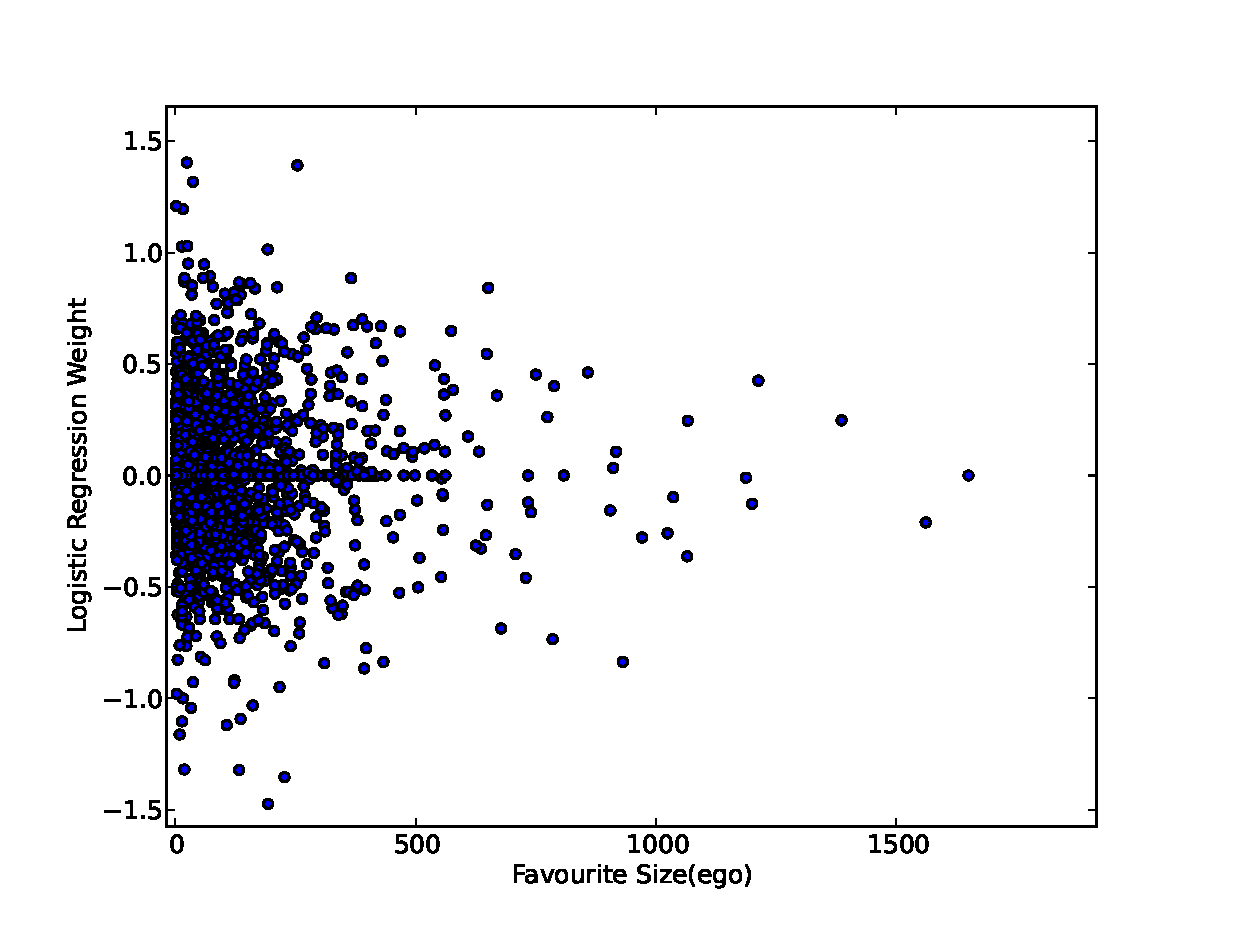
\includegraphics[width=40mm, height=30mm]{data/plots/scatterplots/LRweights/LRweightvsPageEgoSize.eps}}
\subfloat[Fig: logistic regression coefficients vs favourite size(ego) ][LR coefficient vs favourite(ego)]{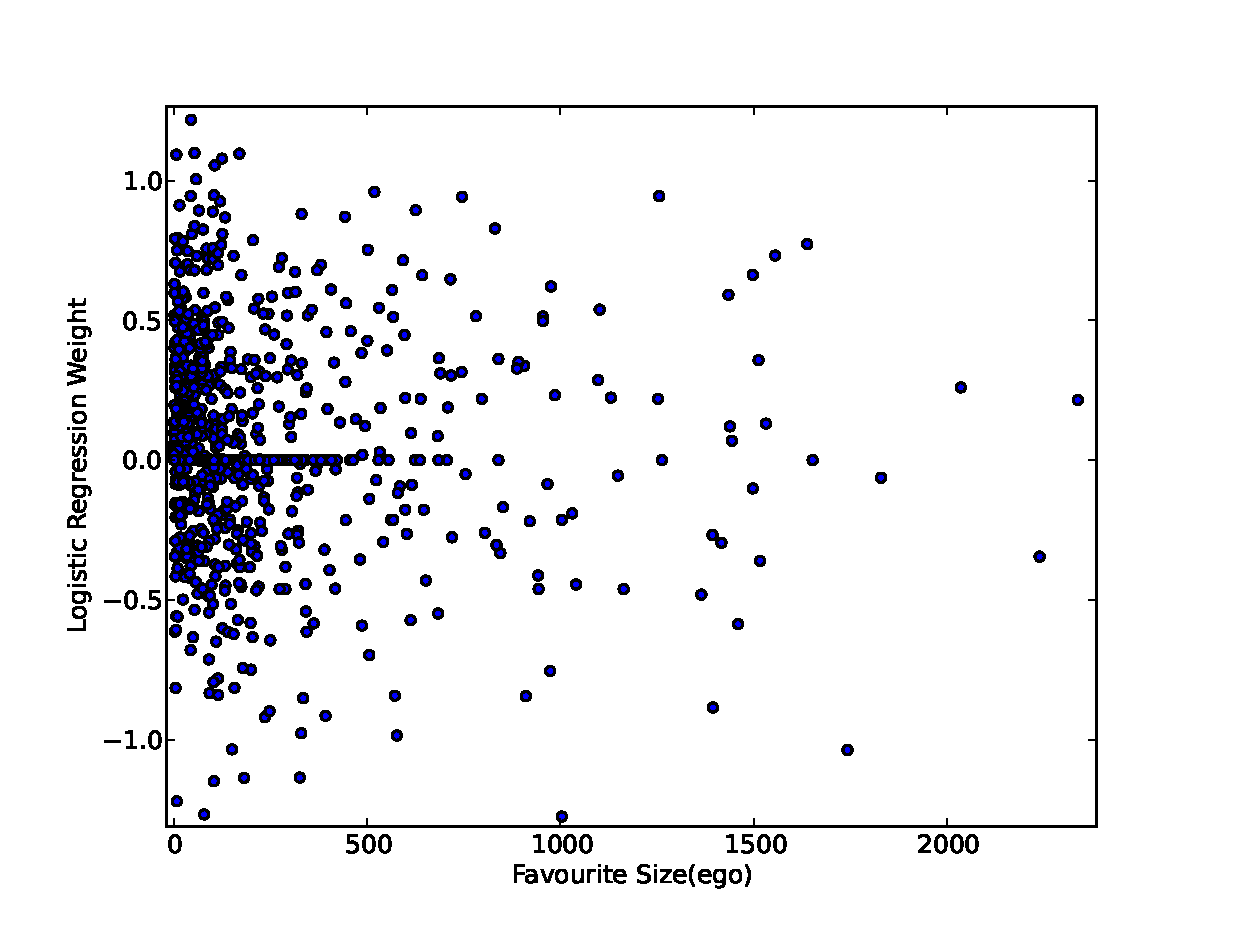
\includegraphics[width=40mm, height=30mm]{data/plots/scatterplots/LRweights/LRweightvsFavouriteEgoSize.eps}}
\end{tabular}
\caption{ logistic regression coefficients   vs size}
\label{Fig: logistic regression coefficients   vs size}
\end{figure*}


\begin{figure*}[h]
\centering
\begin{tabular}{ccc}
\subfloat[Fig: conditional entropy vs size][CE vs size(top 500)]{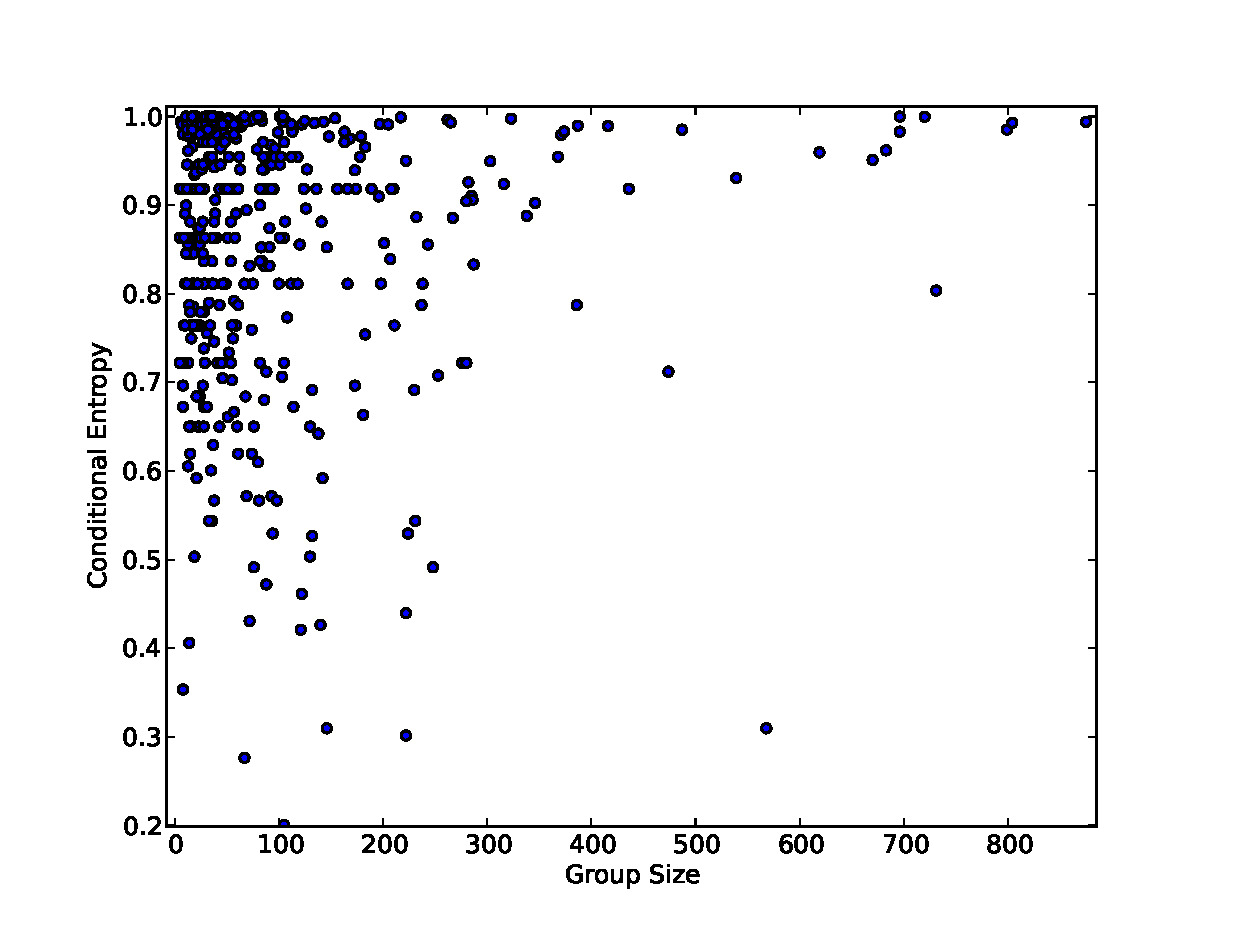
\includegraphics[width=40mm, height=30mm]{data/plots/scatterplots/sortedBySE/CEvsGroupSize.eps}}
\subfloat[Fig: conditional entropy vs size][CE vs size(top 1000)]{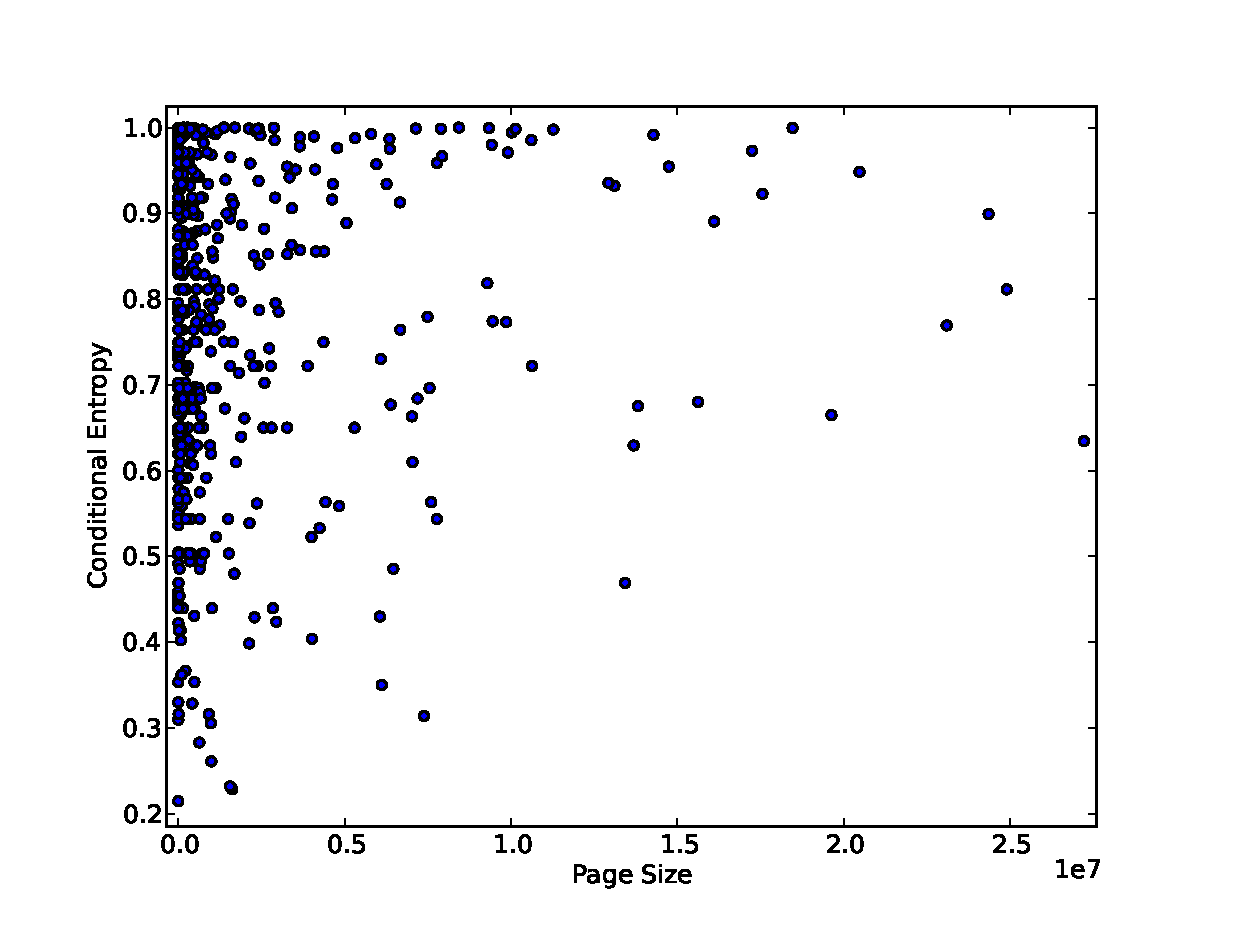
\includegraphics[width=40mm, height=30mm]{data/plots/scatterplots/sortedBySE/CEvsPageSize.eps}}
\subfloat[Fig: conditional entropy vs size][CE vs size(top 800)]{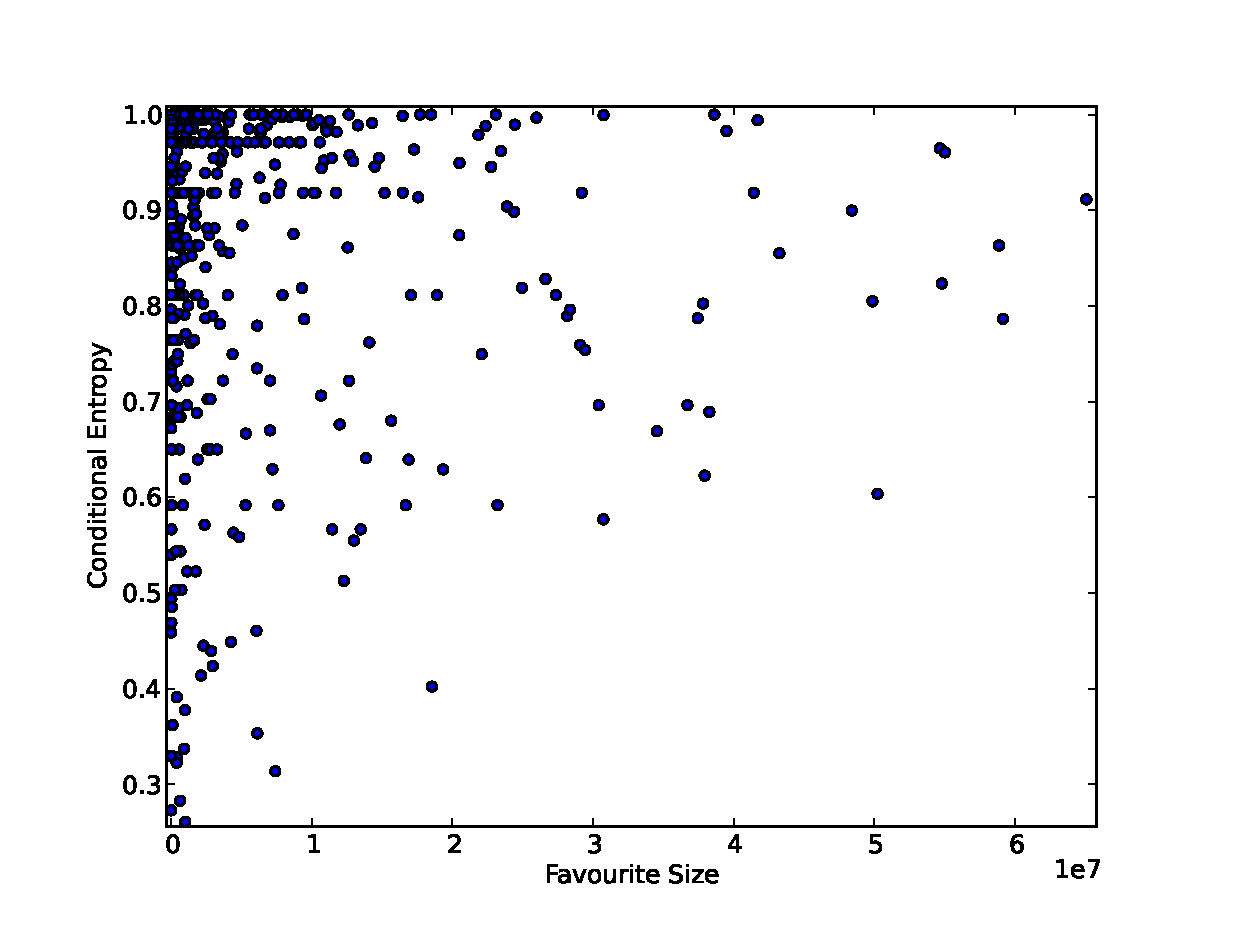
\includegraphics[width=40mm, height=30mm]{data/plots/scatterplots/sortedBySE/CEvsfavSize.eps}} \\
\subfloat[Fig: mutual information vs size][MI vs size(top 500)]{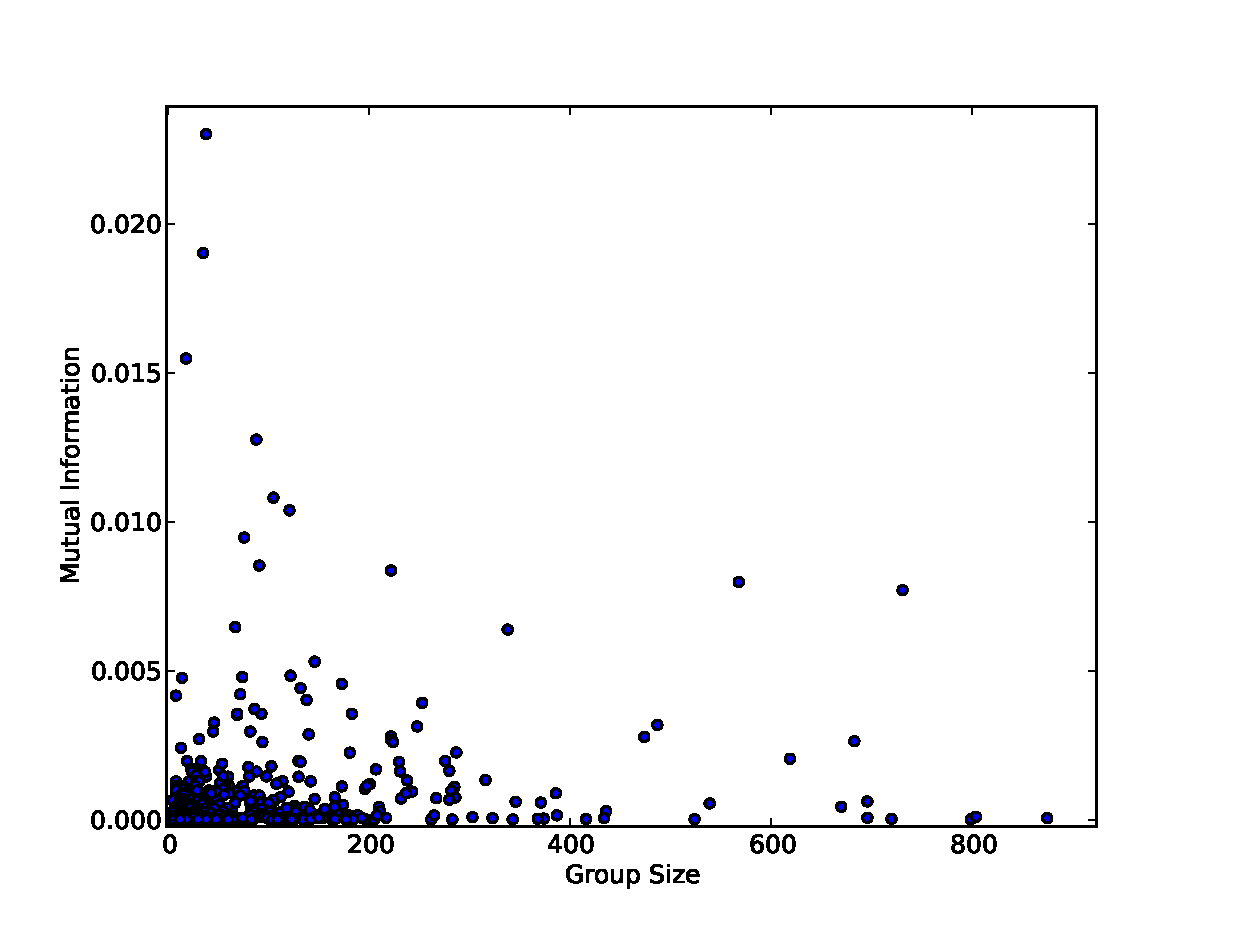
\includegraphics[width=40mm, height=30mm]{data/plots/scatterplots/sortedBySE/MIvsGroupSize.eps}}
\subfloat[Fig: mutual information vs size][MI vs size(top 1000)]{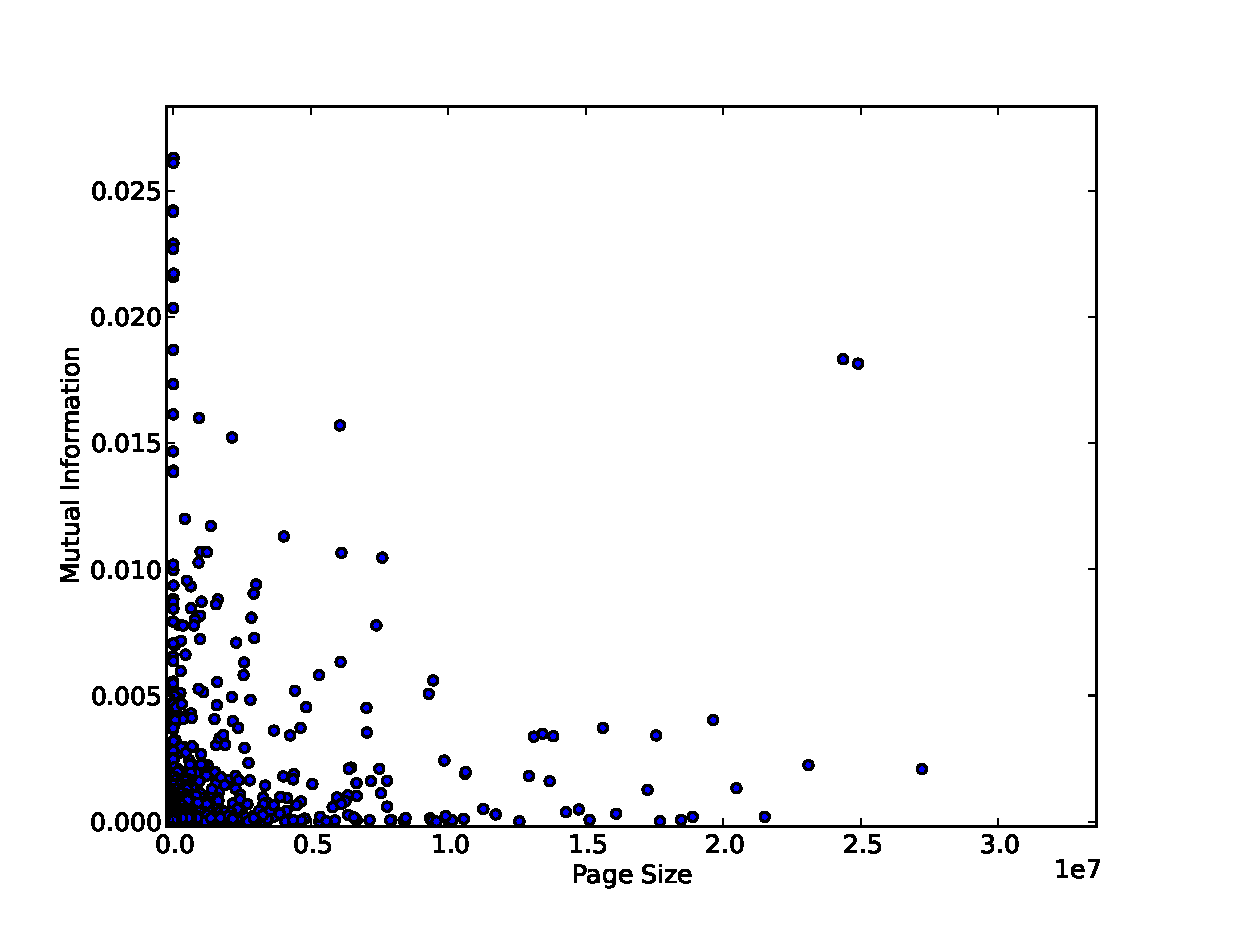
\includegraphics[width=40mm, height=30mm]{data/plots/scatterplots/sortedBySE/MIvsPageSize.eps}}
\subfloat[Fig: mutual information vs size][MI vs size(top 800)]{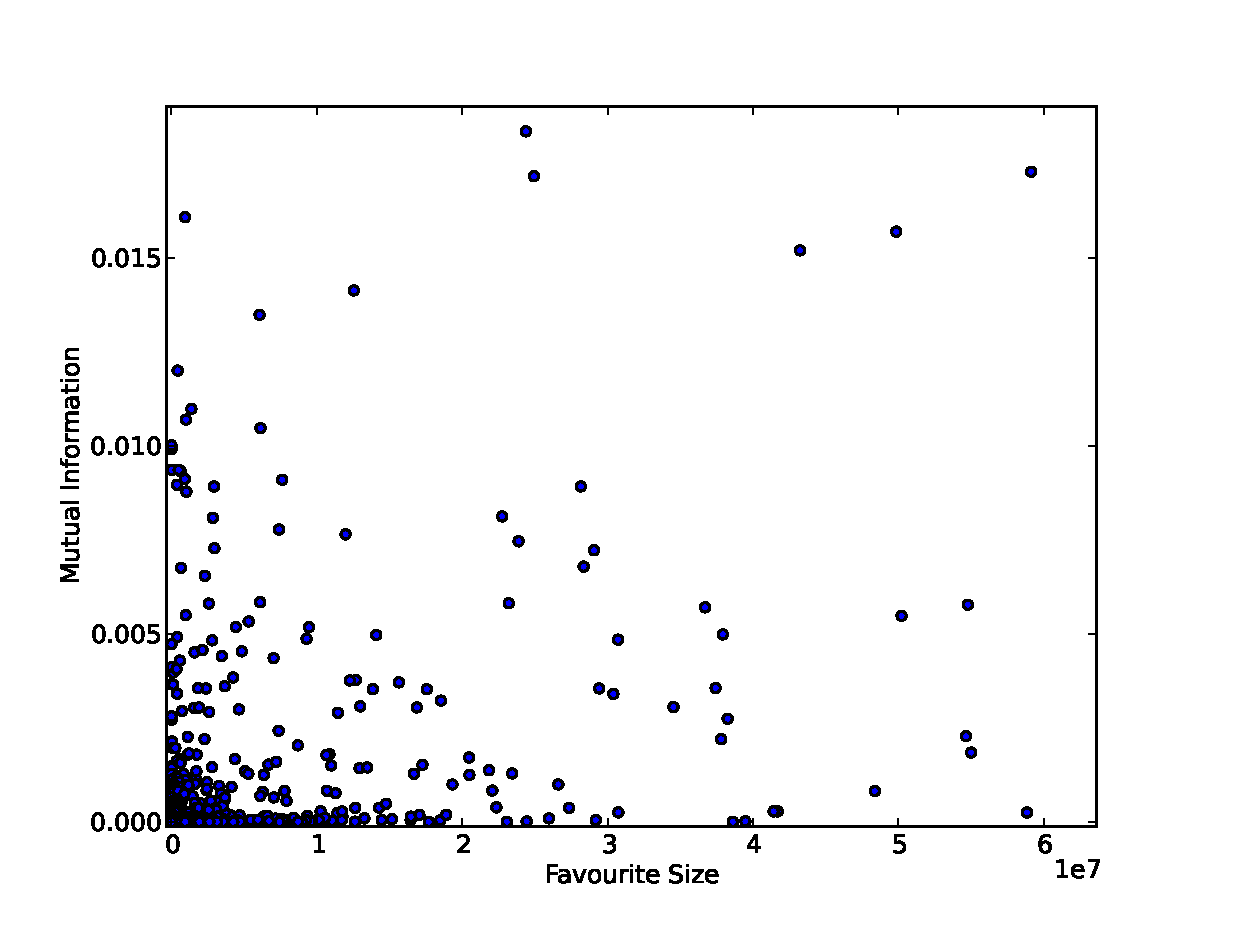
\includegraphics[width=40mm, height=30mm]{data/plots/scatterplots/sortedBySE/MIvsfavSize.eps}}
\end{tabular}
\caption{ conditional entropy/mutual information vs size (top k sorted by standard error)}
\label{Fig:  conditional entropy/mutual information vs size (top k sorted by standard error)}
\end{figure*}

\begin{figure*}[h]
\centering
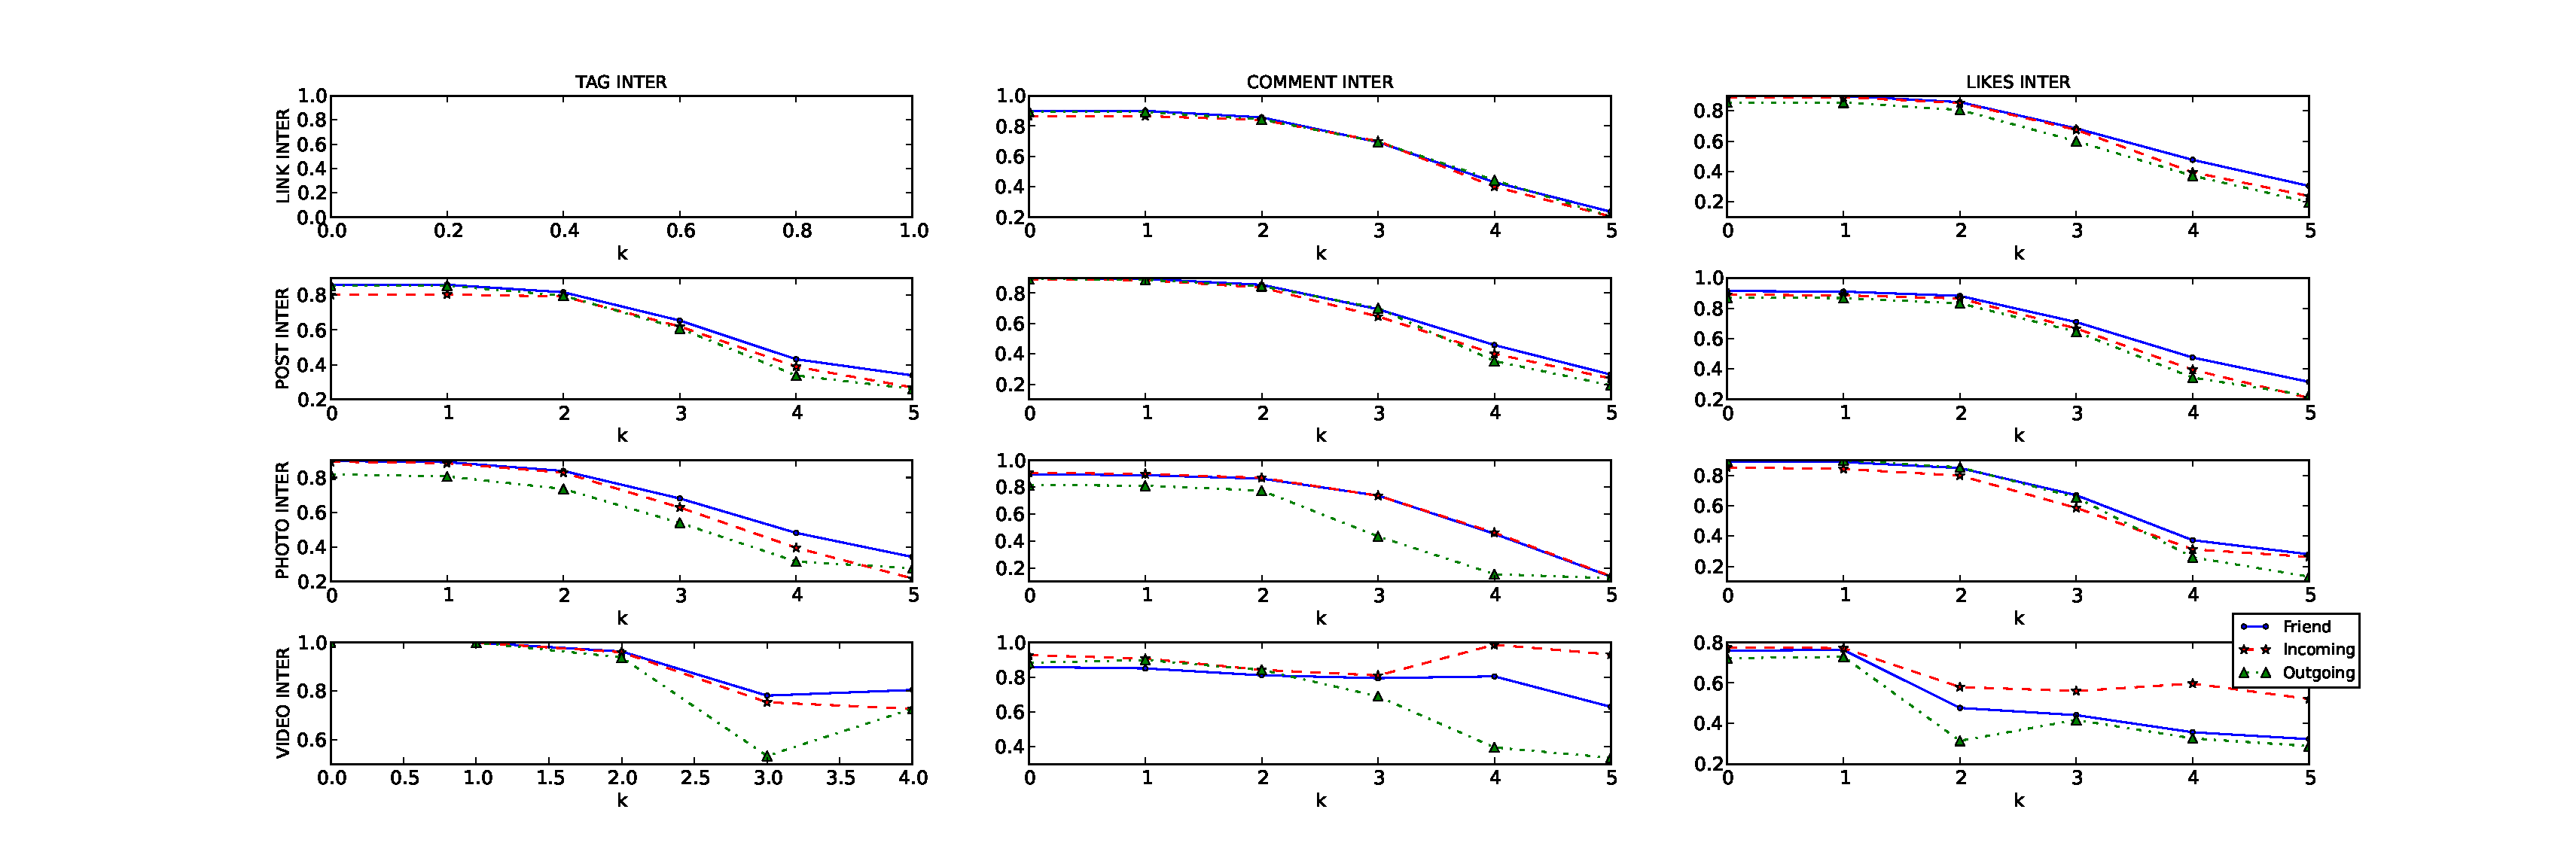
\includegraphics[scale=0.25]{data/plots/vsk/CEvsK.eps}
\caption{All graph plots Conditional Entropy for interaction actions vs Interaction modalities. Each graph analyzes different Interaction Directionality  }
\end{figure*}

\cleardoublepage
\begin{table}
	\centering
	\begin{tabular}{| >{\small}l | >{\small}r | >{\small}r | >{\small}r | >{\small}r | >{\small}r | >{\small}r |}
		\hline
		Modality & ConditionalEntropy & (Like,True) & (Dislike,True) & (Like,False) & (Dislike,False) & P(like|True)\\
		\hline
		\textbf{video} & 0.850116919421 & 117 & 44 & 2402 & 2962 & 0.7267\\
		\hline
		\textbf{link} & 0.914700608855 & 989 & 486 & 1530 & 2520 & 0.6705\\
		\hline
		\textbf{post} & 0.918160390299 & 1154 & 576 & 1365 & 2430 & 0.6671\\
		\hline
		\textbf{photo} & 0.9259513318 & 675 & 349 & 1844 & 2657 & 0.6591\\
		\hline
		\hline
		\textbf{Modality} & MutualInformation & (Like,True) & (Dislike,True) & (Like,False) & (Dislike,False) & P(like|True)\\
		\hline
		\textbf{post} & 0.0594688018722 & 1154 & 576 & 1365 & 2430 & 0.6671\\
		\hline
		\textbf{link} & 0.0490133947836 & 989 & 486 & 1530 & 2520 & 0.6705\\
		\hline
		\textbf{photo} & 0.0273700186713 & 675 & 349 & 1844 & 2657 &  0.6591\\
		\hline
		\textbf{video} & 0.0064494273283 & 117 & 44 & 2402 & 2962 & 0.7267\\
		\hline
		\hline
		\textbf{Type}  & Conditional Entropy & (Like,True) & (Dislike,True) & (Like,False) & (Dislike,False)  & P(like|True)\\
		\hline
		\textbf{Tags}  &  0.919971597996 & 809 & 407 & 1710 & 2599 & 0.6653\\
		\hline
		\textbf{Comments}  &  0.921373670369 & 1009 & 511 & 1510 & 2495 & 0.66382\\
		\hline
		\textbf{Likes}  &  0.924414408934 & 1135 & 583 & 1384 & 2423 & 0.6607\\
		\hline
		\hline
		\textbf{Type}  & Mutual Information & (Like,True) & (Dislike,True) & (Like,False) & (Dislike,False)  & P(like|True)\\
		\hline
		\textbf{Likes}  &  0.0553328447681 & 1135 & 583 & 1384 & 2423 & 0.6607\\
		\hline
		\textbf{Comments}  &  0.0479360954681 & 1009 & 511 & 1510 & 2495 & 0.66382\\
		\hline
		\textbf{Tags}  &  0.0361031572103 & 809 & 407 & 1710 & 2599 & 0.6653\\
		\hline
		\hline
		\textbf{Direction} & Mutual Information & (Like,True) & (Dislike,True) & (Like,False) & (Dislike,False)  & P(like|True)\\
		\hline
		\textbf{Outgoing}  &  0.049470651248 & 1074 & 562 & 1445 & 2444 &  0.6565\\
		\hline
		\textbf{Incoming}  &  0.0470981200647 & 1081 & 584 & 1438 & 2422 & 0.64924\\
		\hline
		\hline
		\textbf{Direction} & Conditional Entropy &  (Like,True) & (Dislike,True) & (Like,False) & (Dislike,False)  & P(like|True)\\
		\hline
		\textbf{Outgoing}  &  0.928353525673 & 1074 & 562 & 1445 & 2444 & 0.6565\\
		\hline
		\textbf{Incoming}  &  0.934921690705 & 1081 & 584 & 1438 & 2422 & 0.64924\\
		\hline
	\end{tabular}
\end{table}
		
	
\cleardoublepage
\begin{table}
	\centering
	\begin{tabular}{| >{\small}l | >{\small}r | >{\small}r | >{\small}r | >{\small}r | >{\small}r | >{\small}r |}
		\hline
		Interaction & Conditional Entropy & (Like,True) & (Dislike,True) & (Like,False) & (Dislike,False)  & P(like|True)\\
		\hline
		TAGS\_OUTGOING & 0.885214556947 & 661 & 287 & 1858 & 2719  & 0.6973\\
		LIKES\_OUTGOING & 0.885367017942 & 911 & 396 & 1608 & 2610 & 0.6970\\
		TAGS\_INCOMING & 0.899959283697 & 653 & 301 & 1866 & 2705 & 0.6845\\
		LIKES\_INCOMING & 0.901653997367 & 986 & 458 & 1533 & 2548 & 0.6828\\
		COMMENTS\_OUTGOING & 0.908080562132 & 790 & 377 & 1729 & 2629 & 0.6769\\
		COMMENTS\_INCOMING & 0.911567201865 & 840 & 407 & 1679 & 2599 & 0.6736\\
		\hline
		\hline
		Interaction & Mutual Information & (Like,True) & (Dislike,True) & (Like,False) & (Dislike,False)& P(like|True)\\		
		\hline
		LIKES\_INCOMING & 0.0532717033854 & 986 & 458 & 1533 & 2548 &  0.6828\\
		LIKES\_OUTGOING & 0.0527680578968 & 911 & 396 & 1608 & 2610 & 0.6970\\
		COMMENTS\_INCOMING & 0.0402962708309 & 840 & 407 & 1679 & 2599 & 0.6736\\
		COMMENTS\_OUTGOING & 0.0381700399797 & 790 & 377 & 1729 & 2629 & 0.6769\\
		TAGS\_OUTGOING & 0.035303106185 & 661 & 287 & 1858 & 2719 & 0.6973\\
		TAGS\_INCOMING & 0.0318329570229 & 653 & 301 & 1866 & 2705 & 0.6845\\
		\hline
		
		Interaction & Conditional Entropy & (Like,True) & (Dislike,True) & (Like,False) & (Dislike,False)  & P(like|True)\\
		\hline
		PHOTO\_OUTGOING & 0.856939074179 & 521 & 203 & 1998 & 2803 & 0.7196\\
		VIDEO\_OUTGOING & 0.863258948786 & 69 & 27 & 2450 & 2979 & 0.7188\\
		LINK\_OUTGOING & 0.895377102746 & 809 & 366 & 1710 & 2640 & 0.6885\\
		LINK\_INCOMING & 0.895672876337 & 797 & 361 & 1722 & 2645 & 0.6882\\
		POST\_INCOMING & 0.901803982795 & 1007 & 468 & 1512 & 2538 & 0.6827\\
		POST\_OUTGOING & 0.905555107759 & 1006 & 475 & 1513 & 2531 & 0.6793\\
		VIDEO\_INCOMING & 0.915141339321 & 68 & 33 & 2451 & 2973 & 0.8395\\
		PHOTO\_INCOMING & 0.920746179598 & 563 & 284 & 1956 & 2722 & 0.6647\\
		\hline
		\hline
		Interaction & Mutual Information & (Like,True) & (Dislike,True) & (Like,False) & (Dislike,False)& P(like|True)\\
		\hline
		POST\_INCOMING & 0.0547156102171 & 1007 & 468 & 1512 & 2538 & 0.6827\\
		POST\_OUTGOING & 0.0533330284575 & 1006 & 475 & 1513 & 2531  & 0.6793\\
		LINK\_OUTGOING & 0.0426702641841 & 809 & 366 & 1710 & 2640 & 0.6885\\
		LINK\_INCOMING & 0.0417931651624 & 797 & 361 & 1722 & 2645 & 0.6883\\
		PHOTO\_OUTGOING & 0.0307864066352 & 521 & 203 & 1998 & 2803 & 0.7196\\
		PHOTO\_INCOMING & 0.0229340503984 & 563 & 284 & 1956 & 2722 & 0.6647\\
		VIDEO\_OUTGOING & 0.0035452127605 & 69 & 27 & 2450 & 2979 & 0.7188\\
		VIDEO\_INCOMING & 0.00253337061407 & 68 & 33 & 2451 & 2973 & 0.8395\\
		\hline
				
	\end{tabular}
\end{table}

\begin{table}
	\centering
	\begin{tabular}{| >{\small}l | >{\small}r | >{\small}r | >{\small}r | >{\small}r | >{\small}r | >{\small}r |}
	\hline
	Interaction & Conditional Entropy & (Like,True) & (Dislike,True) & (Like,False) & (Dislike,False)  & P(like|True)\\
	\hline
	\textbf{VIDEO\_LIKES\_OUTGOING} & 0.722397472066 & 31 & 7 & 2488 & 2999 & 0.8158\\
	\hline
	\textbf{VIDEO\_LIKES\_INCOMING} & 0.775086171837 & 43 & 12 & 2476 & 2994 & 0.7818\\
	\hline
	\textbf{POST\_TAGS\_INCOMING} & 0.802855788214 & 444 & 143 & 2075 & 2863 & 0.7564\\
	\hline
	\textbf{PHOTO\_COMMENTS\_OUTGOING} & 0.816036600382 & 135 & 45 & 2384 & 2961 & 0.75\\
	\hline
	\textbf{PHOTO\_TAGS\_OUTGOING} & 0.818540125915 & 427 & 145 & 2092 & 2861 & 0.7465\\
	\hline
	\textbf{PHOTO\_LIKES\_INCOMING} & 0.853009353418 & 277 & 106 & 2242 & 2900 & 0.7232\\
	\hline
	\textbf{LINK\_LIKES\_OUTGOING} & 0.855368864256 & 728 & 282 & 1791 & 2724 & 0.7208\\
	\hline
	\textbf{POST\_TAGS\_OUTGOING} & 0.856163233945 & 505 & 196 & 2014 & 2810 & 0.7204\\
	\hline
	\textbf{LINK\_COMMENTS\_INCOMING} & 0.865533720447 & 530 & 213 & 1989 & 2793 & 0.7133 \\
	\hline
	\textbf{POST\_LIKES\_OUTGOING} & 0.870618130159 & 834 & 342 & 1685 & 2664 & 0.7092\\
	\hline
	\textbf{VIDEO\_COMMENTS\_OUTGOING} & 0.883596675997 & 43 & 18 & 2476 & 2988 & 0.7049\\
	\hline
	\textbf{LINK\_LIKES\_INCOMING} & 0.888406184542 & 742 & 326 & 1777 & 2680 & 0.6948\\
	\hline
	\textbf{POST\_LIKES\_INCOMING} & 0.889444522106 & 929 & 410 & 1590 & 2596 & 0.6938\\
	\hline
	\textbf{POST\_COMMENTS\_INCOMING} & 0.890449138325 & 763 & 338 & 1756 & 2668 & 0.6930\\
	\hline
	\textbf{PHOTO\_TAGS\_INCOMING} & 0.890856994354 & 485 & 215 & 2034 & 2791 & 0.6928\\
	\hline
	\textbf{POST\_COMMENTS\_OUTGOING} & 0.894129257133 & 694 & 312 & 1825 & 2694 & 0.6899\\
	\hline
	\textbf{LINK\_COMMENTS\_OUTGOING} & 0.895134128697 & 543 & 245 & 1976 & 2761 & 0.6891\\
	\hline
	\textbf{PHOTO\_LIKES\_OUTGOING} & 0.89759612767 & 161 & 73 & 2358 & 2933 & 0.6880\\
	\hline
	\textbf{PHOTO\_COMMENTS\_INCOMING} & 0.906541518549 & 290 & 137 & 2229 & 2869 & 0.6792\\
	\hline
	\textbf{VIDEO\_COMMENTS\_INCOMING} & 0.92652449307 & 53 & 27 & 2466 & 2979 & 0.6625\\
	\hline
	\textbf{FRIENDS} & 0.965942963751 & 1392 & 895 & 1127 & 2111 & 0.6087\\
	\hline
	\textbf{VIDEO\_TAGS\_INCOMING} & 0.999999611934 & 17 & 17 & 2502 & 2989 & 0.5\\
	\hline
	\textbf{VIDEO\_TAGS\_OUTGOING} & 0.999999611934 & 16 & 16 & 2503 & 2990 & 0.5\\
	\hline
	\end{tabular}
\end{table}

\cleardoublepage

\begin{table}
	\centering
	\begin{tabular}{| >{\small}l | >{\small}r | >{\small}r | >{\small}r | >{\small}r | >{\small}r | >{\small}r |}
	\hline
	Interaction & Mutual Information & (Like,True) & (Dislike,True) & (Like,False) & (Dislike,False)& P(like|True)\\
	\hline
	\textbf{POST\_LIKES\_INCOMING} & 0.0524561740233 & 929 & 410 & 1590 & 2596 & 0.6938\\
	\hline
	\textbf{POST\_LIKES\_OUTGOING}& 0.050407410911 & 834 & 342 & 1685 & 2664 & 0.7092\\
	\hline
	\textbf{FRIENDS} & 0.0473539909731 & 1392 & 895 & 1127 & 2111 & 0.6087\\
	\hline
	\textbf{LINK\_LIKES\_OUTGOING}& 0.0457244144031 & 728 & 282 & 1791 & 2724 & 0.7208\\
	\hline
	\textbf{POST\_COMMENTS\_INCOMING}& 0.0405155210996 & 763 & 338 & 1756 & 2668& 0.6930\\
	\hline
	\textbf{LINK\_LIKES\_INCOMING}& 0.0396004717225 & 742 & 326 & 1777 & 2680 & 0.6948\\
	\hline
	\textbf{POST\_COMMENTS\_OUTGOING}& 0.0352609340207 & 694 & 312 & 1825 & 2694 & 0.6899\\
	\hline
	\textbf{POST\_TAGS\_INCOMING}& 0.0315770377754 & 444 & 143 & 2075 & 2863 & 0.7564\\
	\hline
	\textbf{LINK\_COMMENTS\_INCOMING}& 0.0299391900579 & 530 & 213 & 1989 & 2793 & 0.7133 \\
	\hline
	\textbf{POST\_TAGS\_OUTGOING}& 0.0296108833783 & 505 & 196 & 2014 & 2810 & 0.7204\\
	\hline
	\textbf{PHOTO\_TAGS\_OUTGOING}& 0.0286060075004 & 427 & 145 & 2092 & 2861 & 0.7465\\
	\hline
	\textbf{LINK\_COMMENTS\_OUTGOING}& 0.0261662648974 & 543 & 245 & 1976 & 2761 & 0.6891\\
	\hline
	\textbf{PHOTO\_TAGS\_INCOMING}& 0.0235803030398 & 485 & 215 & 2034 & 2791 & 0.6928\\
	\hline
	\textbf{PHOTO\_LIKES\_INCOMING}& 0.0155060725343 & 277 & 106 & 2242 & 2900 & 0.7232\\
	\hline
	\textbf{PHOTO\_COMMENTS\_INCOMING}& 0.0120447345005 & 290 & 137 & 2229 & 2869 & 0.6792\\
	\hline
	\textbf{PHOTO\_COMMENTS\_OUTGOING}& 0.00851951888057 & 135 & 45 & 2384 & 2961& 0.75\\
	\hline
	\textbf{PHOTO\_LIKES\_OUTGOING}& 0.00687365820792 & 161 & 73 & 2358 & 2933 & 0.6880\\
	\hline
	\textbf{VIDEO\_LIKES\_INCOMING}& 0.00309679794205 & 43 & 12 & 2476 & 2994 & 0.7818\\
	\hline
	\textbf{VIDEO\_LIKES\_OUTGOING}& 0.00259896191026 & 31 & 7 & 2488 & 2999 & 0.8158\\
	\hline
	\textbf{VIDEO\_COMMENTS\_OUTGOING}& 0.00197259388552 & 43 & 18 & 2476 & 2988 & 0.7049\\
	\hline
	\textbf{VIDEO\_COMMENTS\_INCOMING}& 0.0017837362825 & 53 & 27 & 2466 & 2979 & 0.6625\\
	\hline
	\textbf{VIDEO\_TAGS\_INCOMING}& 3.598735115e-05 & 17 & 17 & 2502 & 2989 & 0.5 \\
	\hline
	\textbf{VIDEO\_TAGS\_OUTGOING}& 3.39757297236e-05 & 16 & 16 & 2503 & 2990 & 0.5\\
	\hline
	\end{tabular}
\end{table}



\cleardoublepage

\begin{table}
\begin{tabular}{| >{\small}l | >{\small}r | >{\small}r | >{\small}r | >{\small}r | >{\small}r |>{\small}r |}
\hline
{} &               id &                                               name &  size &  egosize &  Cond Entropy &  Mutual Information \\
\hline
1057 &  130815873610129 &                                   ANU StalkerSpace &  1292 &     1292 &             0.861615 &            0.030603 \\
778  &  239607379457024 &                                           ANU CSSA &    38 &       38 &             0.745879 &            0.023007 \\
424  &       2397818353 &                                               CSSA &    35 &       35 &             0.600649 &            0.019016 \\
1422 &  215525841848413 &                    Australian National Uni AI \& ML &    18 &       18 &             0.785032 &            0.015477 \\
720  &     324570326277 &  ANU Engineering Students' Association (ANUESA)... &    88 &       88 &             0.471934 &            0.012753 \\
602  &     271451673295 &                                 Canberra Rock Gigs &   105 &      105 &             0.200642 &            0.010805 \\
96   &      11891033953 &  Ekta - Indian Subcontinent Students' Associati... &   121 &      121 &             0.420844 &            0.010377 \\
693  &     219745416919 &  ☠ Heavy Metal - Australian Capital Territory, ... &    30 &       30 &             0.133053 &            0.009798 \\
810  &     213225102082 &             The Great Australian Internet Blackout &    76 &       76 &             0.491275 &            0.009466 \\
865  &     208417795185 &     Stephen Conroy Should Not Filter Our Internet! &    48 &       48 &             0.146109 &            0.008583 \\
1232 &      69858518886 &                         Our Hero: Clem Baker-Finch &    91 &       91 &             0.852441 &            0.008526 \\
707  &       2259054917 &           i feel my phone vibrate when it doesn't. &   222 &      222 &             0.301406 &            0.008358 \\
272  &     121627904865 &                          Lift ACT ban on fireworks &   568 &      568 &             0.309571 &            0.007971 \\
174  &       2336048220 &                  I grew up in Australia in the 90s &   731 &      731 &             0.803557 &            0.007696 \\
1399 &  130385273640777 &                                  Silicone Stripper &    17 &       17 &             0.162342 &            0.007374 \\
914  &     105714109273 &                                     Canberra Music &    67 &       67 &             0.276221 &            0.006458 \\
387  &  243732165652389 &                                      iDiscount ANU &   338 &      338 &             0.887847 &            0.006378 \\
603  &     300607567325 &                    Hardcore dancing is not moshing &     8 &        8 &             0.179274 &            0.006372 \\
394  &     206485584139 &  Metal bands come to Canberra cause I'm sick of... &    12 &       12 &             0.187194 &            0.005973 \\
90   &      19689998305 &       1,000,000 Strong Against High School Musical &   146 &      146 &             0.309571 &            0.005299 \\
\hline
\end{tabular}
\caption{Top 20 Group ranked by Mutual Information}
\label {Top 20 Group ranked by Mutual Information}
\end{table}


\cleardoublepage
\begin{table}
\begin{tabular}{| >{\small}l | >{\small}r | >{\small}r | >{\small}r | >{\small}r | >{\small}r |>{\small}r |}
\hline
{} &               id &                                               name &      size &  egosize &   Cond Entropy &  Mutual Information \\
\hline
1091 &     148551616293 &                 The Australian National University &     10522 &      917 &             0.926747 &            0.026323 \\
2268 &     399805615144 &  Australian National University Students' Assoc... &      3059 &      389 &             0.788451 &            0.026124 \\
4050 &     192286270282 &                            Humans vs Zombies @ ANU &       554 &      212 &             0.841817 &            0.024231 \\
3706 &  174936642528981 &  ANU Engineering Students' Association 2011 (AN... &       285 &      141 &             0.504845 &            0.024180 \\
128  &  192078840839006 &                                   ANU Stalkerspace &      5085 &     1065 &             0.948173 &            0.022915 \\
3047 &  207140035973127 &  ANU Computer Science Students' Association (AN... &       165 &       85 &             0.873524 &            0.022711 \\
4456 &  105586819475691 &                     Australian National University &     11622 &      454 &             0.783520 &            0.021732 \\
3202 &  159352257471339 &                                          ANU ducks &      1445 &      372 &             0.858136 &            0.021594 \\
2858 &  254743647903977 &                                  Robogals Canberra &       135 &       32 &             0.501452 &            0.020362 \\
3240 &  293434554026394 &                ANU O-Week 2012: Escape to the East &      1483 &      240 &             0.829381 &            0.018705 \\
3055 &      22934684677 &                                The Big Bang Theory &  24355106 &     2552 &             0.899177 &            0.018333 \\
4083 &       9588466619 &                                           Futurama &  24899564 &     1213 &             0.811316 &            0.018158 \\
3780 &  171648066192062 &                                            ANU XSA &       421 &      123 &             0.858345 &            0.017345 \\
1828 &  157065757691727 &                               Angie To Photography &       203 &       63 &             0.646059 &            0.016147 \\
1046 &     494637910144 &                                       The IT Crowd &    936956 &      578 &             0.793751 &            0.016003 \\
63   &      28627688223 &                                        MythBusters &   6059381 &      648 &             0.429793 &            0.015709 \\
3429 &     290539813359 &                        Trust Me, I'm an "Engineer" &   2139099 &      283 &             0.538777 &            0.015233 \\
1736 &  264476006941706 &                                          Potential &       116 &       37 &             0.214530 &            0.014676 \\
3768 &  221086387944225 &                    ANU/Canberra Python Social Club &        21 &        9 &             0.741611 &            0.013916 \\
2855 &     273323547059 &                             ANUSA Euro O-Week 2010 &      1453 &      428 &             0.546198 &            0.013857 \\
\hline
\end{tabular}
\caption{Top 20 Page ranked by Mutual Information}
\label {Top 20 Page ranked by Mutual Information}
\end{table}

\cleardoublepage

\begin{table}
\begin{tabular}{| >{\small}l | >{\small}r | >{\small}r | >{\small}r | >{\small}r | >{\small}r |>{\small}r |}
\hline
{} &               id &                 name &      size &  egosize &  cond entropy &  mutual information \\
\hline
1620 &      22934684677 &  the big bang theory &  24382711 &     2339 &             0.898472 &            0.018366 \\
558  &      29534858696 &         the simpsons &  59144063 &     1439 &             0.786530 &            0.017291 \\
1546 &       9588466619 &             futurama &  24939188 &     1131 &             0.818993 &            0.017171 \\
630  &     494637910144 &         the it crowd &    937445 &      565 &             0.790827 &            0.016082 \\
1678 &      24609282673 &           family guy &  49865912 &     2036 &             0.804842 &            0.015698 \\
37   &       6708787004 &           south park &  43243922 &     1444 &             0.855054 &            0.015199 \\
1425 &      29112278285 &               scrubs &  12543319 &     1532 &             0.861083 &            0.014135 \\
24   &      28627688223 &          mythbusters &   6060917 &      597 &             0.460559 &            0.013485 \\
1409 &  163542213701619 &   avascular necrosis &       195 &       36 &             0.114687 &            0.012040 \\
1304 &      21570237112 &       blind guardian &    422327 &       54 &             0.328430 &            0.012004 \\
328  &     292772493767 &             tortured &      1082 &       32 &             0.120693 &            0.011223 \\
685  &  115344841825821 &              elysian &      3195 &       36 &             0.120693 &            0.011223 \\
1687 &      76613428183 &            community &   1369762 &      304 &             0.760992 &            0.010984 \\
230  &       7496603409 &                opeth &    997062 &      155 &             0.260887 &            0.010700 \\
1372 &      19058419696 &              pantera &   6125926 &      220 &             0.353390 &            0.010469 \\
39   &  149992358386897 &          anno domini &      6306 &       21 &             0.127431 &            0.010408 \\
745  &  108511629178228 &          hellbringer &      1533 &       25 &             0.129247 &            0.010204 \\
1388 &     170724093400 &      johnny roadkill &       973 &       25 &             0.129247 &            0.010204 \\
1445 &      17222896745 &          darker half &     12964 &       25 &             0.129247 &            0.010204 \\
848  &     186487216175 &     robert the bruce &       220 &       69 &             0.539975 &            0.010013 \\
\hline
\end{tabular}
\caption{Top 20 Favourite ranked by Mutual Information}
\label {Top 20 Favourite ranked by Mutual Information}
\end{table}


\cleardoublepage
\begin{table}
\begin{tabular}{| >{\small}l | >{\small}r | >{\small}r | >{\small}r | >{\small}r | >{\small}r |>{\small}r |}
\hline
{} &               id &                                               name &  size &  egosize &  conditional Entropy &  Mutual Information \\
\hline
693  &     219745416919 &  ☠ Heavy Metal - Australian Capital Territory, ... &    30 &       30 &             0.133053 &            0.009798 \\
865  &     208417795185 &     Stephen Conroy Should Not Filter Our Internet! &    48 &       48 &             0.146109 &            0.008583 \\
1399 &  130385273640777 &                                  Silicone Stripper &    17 &       17 &             0.162342 &            0.007374 \\
603  &     300607567325 &                    Hardcore dancing is not moshing &     8 &        8 &             0.179274 &            0.006372 \\
394  &     206485584139 &  Metal bands come to Canberra cause I'm sick of... &    12 &       12 &             0.187194 &            0.005973 \\
602  &     271451673295 &                                 Canberra Rock Gigs &   105 &      105 &             0.200642 &            0.010805 \\
712  &     260400635979 &  Let's Mosh - Canberra metal radio show - 2XX 9... &    22 &       22 &             0.205612 &            0.005178 \\
942  &     375249421929 &                   Bring Steel Panther to Australia &     7 &        7 &             0.205612 &            0.005178 \\
1351 &      24472987632 &            Canberra Death/Heavy Metal Appreciation &    16 &       16 &             0.205612 &            0.005178 \\
683  &     175414921393 &                            Robert The Bruce (Band) &    54 &       54 &             0.222306 &            0.004586 \\
1357 &  122079121158013 &                         Heavy Metal in Canberra !! &    20 &       20 &             0.235215 &            0.004193 \\
313  &       2494134578 &                              Monash Primary School &    23 &       23 &             0.242315 &            0.003997 \\
508  &       6192861590 &              Exploiters of the Music Shop shortcut &    76 &       76 &             0.242315 &            0.003997 \\
802  &       2325864288 &                                       Aust H Metal &    10 &       10 &             0.242315 &            0.003997 \\
1016 &  162541263795239 &                                    ANU ESA Members &    11 &       11 &             0.242315 &            0.003997 \\
1185 &      13913770873 &                                         illuminati &    10 &       10 &             0.242315 &            0.003997 \\
246  &      19062002920 &  If This Group Gets To 100,000 I Will Eat A Bou... &    58 &       58 &             0.258043 &            0.003607 \\
183  &     187121217154 &                          Specialist Maths LTC 2009 &    19 &       19 &             0.266789 &            0.003412 \\
1159 &       2228823181 &  I learnt all my life lessons from the sad bits... &    19 &       19 &             0.266789 &            0.003412 \\
914  &     105714109273 &                                     Canberra Music &    67 &       67 &             0.276221 &            0.006458 \\
\hline
\end{tabular}
\caption{Top 20 Group ranked by Conditional Entropy}
\label {Top 20 Group ranked by Conditional Entropy}
\end{table}

\cleardoublepage
\begin{table}
\begin{tabular}{| >{\small}l | >{\small}r | >{\small}r | >{\small}r | >{\small}r | >{\small}r |>{\small}r |}
\hline
{} &               id &                   name &     size &  egosize &  conditional Entropy &  Mutual Information \\
\hline
3732 &  163542213701619 &     Avascular Necrosis &      195 &       36 &             0.114687 &            0.012040 \\
3876 &  128224467221576 &               Assidian &     1873 &       44 &             0.116127 &            0.011835 \\
875  &     292772493767 &               Tortured &     1080 &       34 &             0.120693 &            0.011223 \\
1840 &  115344841825821 &                Elysian &     3188 &       37 &             0.120693 &            0.011223 \\
3998 &      17222896745 &            Darker Half &    12898 &       28 &             0.120693 &            0.011223 \\
959  &     170724093400 &        Johnny Roadkill &      970 &       30 &             0.123962 &            0.010815 \\
107  &  149992358386897 &            Anno Domini &     6304 &       25 &             0.127431 &            0.010408 \\
926  &  106609569416773 &          Billy Madison &  1378990 &      189 &             0.127431 &            0.010408 \\
2024 &  108511629178228 &            Hellbringer &     1521 &       25 &             0.129247 &            0.010204 \\
4689 &  107950569228237 &          Metalocalypse &   607654 &       87 &             0.133053 &            0.009798 \\
54   &     481263060510 &        Bane Of Isildur &      920 &       12 &             0.137113 &            0.009392 \\
672  &  107790305938800 &              Katabasis &     2751 &       14 &             0.137113 &            0.009392 \\
1681 &       8769188951 &                Turisas &   189152 &       29 &             0.137113 &            0.009392 \\
2913 &  154602167894995 &          Aeon of Horus &     2619 &       40 &             0.137113 &            0.009392 \\
2578 &  155961171094428 &           Better Music &      717 &       43 &             0.141455 &            0.008987 \\
2784 &       8216149897 &        Ne Obliviscaris &    12873 &       18 &             0.141455 &            0.008987 \\
1157 &  131572223581891 &  Led Zeppelin Official &  7434089 &      314 &             0.143741 &            0.008785 \\
3085 &       7890846826 &                  Edguy &   241190 &       28 &             0.143741 &            0.008785 \\
735  &  133307246745003 &          Jimmy McGrath &       88 &       11 &             0.148564 &            0.008381 \\
2251 &     117564953823 &            HEAVY METAL &    83252 &       21 &             0.148564 &            0.008381 \\
\hline
\end{tabular}
\caption{Top 20 Page ranked by Conditional Entropy}
\label {Top 20 Page ranked by Conditional Entropy}
\end{table}
\cleardoublepage
\begin{table}
\begin{tabular}{| >{\small}l | >{\small}r | >{\small}r | >{\small}r | >{\small}r | >{\small}r |>{\small}r |}
\hline
{} &               id &                      name &    size &  egosize &  conditional Entropy &  Mutual Information \\
\hline
1409 &  163542213701619 &        Avascular Necrosis &     195 &       36 &             0.114687 &            0.012040 \\
328  &     292772493767 &                  Tortured &    1082 &       32 &             0.120693 &            0.011223 \\
685  &  115344841825821 &                   Elysian &    3195 &       36 &             0.120693 &            0.011223 \\
39   &  149992358386897 &               Anno Domini &    6306 &       21 &             0.127431 &            0.010408 \\
745  &  108511629178228 &               Hellbringer &    1533 &       25 &             0.129247 &            0.010204 \\
1388 &     170724093400 &           Johnny Roadkill &     973 &       25 &             0.129247 &            0.010204 \\
1445 &      17222896745 &               Darker Half &   12964 &       25 &             0.129247 &            0.010204 \\
20   &     481263060510 &           Bane Of Isildur &     923 &       12 &             0.137113 &            0.009392 \\
247  &  107790305938800 &                 Katabasis &    2754 &       13 &             0.137113 &            0.009392 \\
759  &  154602167894995 &             Aeon of Horus &    2622 &       35 &             0.137113 &            0.009392 \\
625  &       8769188951 &                   Turisas &  189507 &       24 &             0.139247 &            0.009190 \\
1046 &       8216149897 &           Ne Obliviscaris &   12929 &       16 &             0.141455 &            0.008987 \\
1775 &  107950569228237 &             Metalocalypse &  608063 &       77 &             0.141455 &            0.008987 \\
1150 &       7890846826 &                     Edguy &  241626 &       28 &             0.143741 &            0.008785 \\
271  &  133307246745003 &             Jimmy McGrath &      88 &       11 &             0.148564 &            0.008381 \\
582  &  112609095431682 &  The Schoenberg Automaton &    5237 &       14 &             0.153757 &            0.007977 \\
911  &  120174841337841 &                    Hemina &    1560 &       14 &             0.156507 &            0.007776 \\
1633 &     117564953823 &               HEAVY METAL &   83371 &       20 &             0.156507 &            0.007776 \\
566  &     266872843888 &                 Avantasia &  271596 &       20 &             0.159366 &            0.007575 \\
160  &  132168983461762 &         Silicone Stripper &     143 &       12 &             0.165443 &            0.007173 \\
\hline
\end{tabular}
\caption{Top 20 Favourite ranked by Conditional Entropy}
\label {Top 20 Favourite ranked by Conditional Entropy}
\end{table}
	

\section{Related Work}

%\input related-work

\section{Conclusions}

%\input conclusions

%\bibliography{icwsm11_relpred}
\bibliographystyle{aaai}
\end{document}

